\title{Master's thesis}
\author{Aleksander Mendoza}

\documentclass[12pt]{article}
\usepackage{tikz}
\usepackage[utf8]{inputenc}
\usepackage[T1]{fontenc}
\usepackage{lmodern}
\usepackage{amsfonts}
\usepackage{mathrsfs}
\usepackage{centernot}
\usepackage{listings}
\usepackage{mathtools}
\usepackage{xcolor}
\usepackage{amsthm}
\usepackage{amsmath}
\usepackage{amssymb}
\usepackage{tikzit}
\usepackage{siunitx}
\usepackage[hidelinks]{hyperref}
\usepackage{tabularx}
\usepackage{enumitem}
\usepackage{chemformula}
\input{style.tikzstyles}
\def\MakeUppercaseUnsupportedInPdfStrings{\scshape}
\DeclareMathOperator*{\argmax}{argmax}
\DeclareMathOperator*{\argmin}{argmin}
\DeclareMathOperator*{\hot}{hot}
\newtheorem{definition}{Definition}
\newtheorem{theorem}{Theorem}[section]
\newtheorem{corollary}{Corollary}[theorem]
\newtheorem{lemma}[theorem]{Lemma}
\renewcommand{\labelenumii}{\theenumii}
\renewcommand{\theenumii}{\theenumi.\arabic{enumii}.}
\DeclareSIUnit{\molar}{M}
\begin{document}
\maketitle
\lstset{
	basicstyle=\ttfamily,
	mathescape
}


\begin{abstract}
This thesis focuses on investigating the problems of sample inefficiency and catastrophic forgetting in reinforcement learning. It takes inspiration from neuroscience and mathematical foundations of deep learning and Markov decision processes. A new theoretical framework is proposed, which unifies all those fields and provides valuable fundamental insights to the many problems of deep reinforcement learning and beyond. Based on those arguments, a new model of neural networks is proposed, with the aim of learning sparse cognitive maps and formalising some of the computational mechanisms of biological neurons.   
\end{abstract} 
\tableofcontents
\section{Preliminaries}

Modern deep neural networks have achieved a multitude of impressive feats, yet at the same time their intelligence appears to be shallow and inflexible. Perhaps the most challenging is the frontier of reinforcement learning (RL).  As it has been demonstrated in Deepmind's ablation studies \cite{rainbow_dqn}, deep RL requires absurd amounts of training data and computation power (figure \ref{fig:dqn}). This issue is often referred to as sample inefficiency.
\begin{figure}[!htbp]
	\centering
	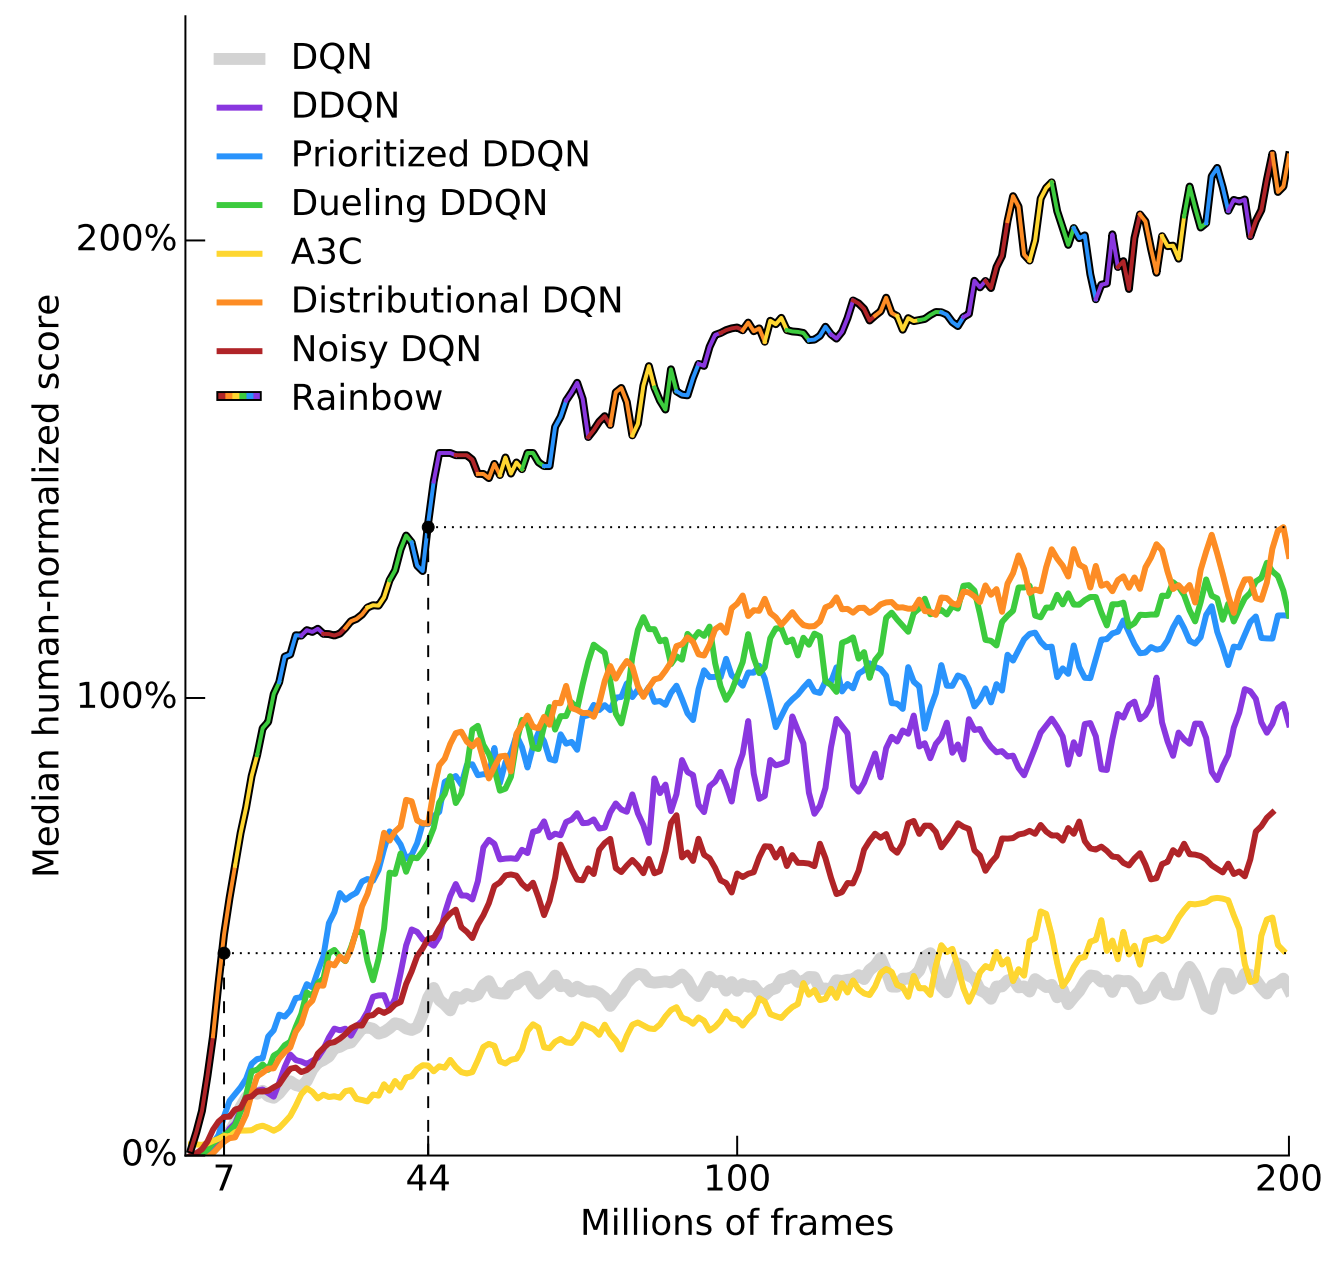
\includegraphics[width=7cm]{dqn}
	\caption{Median human-normalized performance across
		57 Atari games for various deep RL methods.}
	\label{fig:dqn}
\end{figure} 
The produced results rarely generalize to novel tasks and often fail to adapt to slight variations of the same task \cite{generalisation_in_rl}. Transfer learning does not exist in deep RL and fine-tuning an agent on a novel task leads to \textit{catastrophic forgetting} of the previous one. Moreover, even within the same environment, reproducibility suffers and learning algorithms may fail due to random fluctuations \cite{vime}, as it can be seen on figure \ref{fig:vime}. 
\begin{figure}[!htbp]
	\centering
	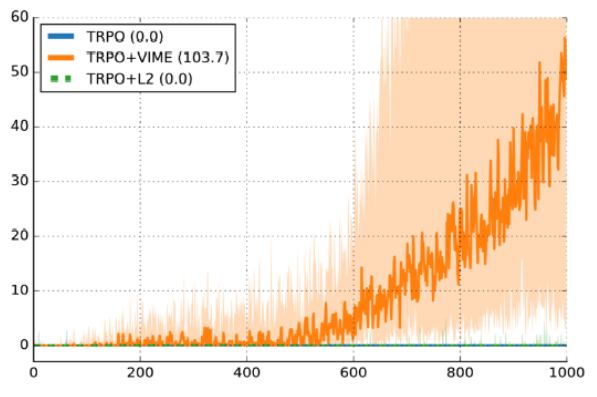
\includegraphics[width=7cm]{vime}
	\caption{The dark line is the median performance over 10 random seeds. The shaded region is the 25th to 75th percentile. It means that 25\% of runs fail due to randomness.}
	\label{fig:vime}
\end{figure} 
Biological brains do not suffer from these problems. In this thesis, I attempt to investigate what nature can tell us about reinforcement learning and how neuroscientific discoveries could be applied in the field of artificial intelligence. How could we solve the problems of sample inefficiency and catastrophic forgetting? Is deep learning the right tool?

\subsection{Neuronal dynamics}

In order to understand how nature tackles the problems of reinforcement learning, first we should understand some fundamentals of neuroscience. 

\subsubsection{Hodgkin-Huxley model}

Like many natural phenomena, biological brains can be modelled at several levels of complexity. The smallest possible scale is microscopic - the biophysics of individual neurons. The evolution of action potential across cell membrane is well understood and can be modelled mathematically with high accuracy. In 1952, Hodgkin and Huxley \cite{hodgkin} were the first to successfully described membrane potentials using differential equations. Their model was able to perfectly fit the observed experimental data (figure \ref{fig:hodgkin_huxley_experiments}). The Hodgkin-Huxley model will serve as the basis for deriving more complex spiking neural networks - a very promising venue for finding potential future alternatives to deep nets.
\begin{figure}[!htbp]
	\centering
	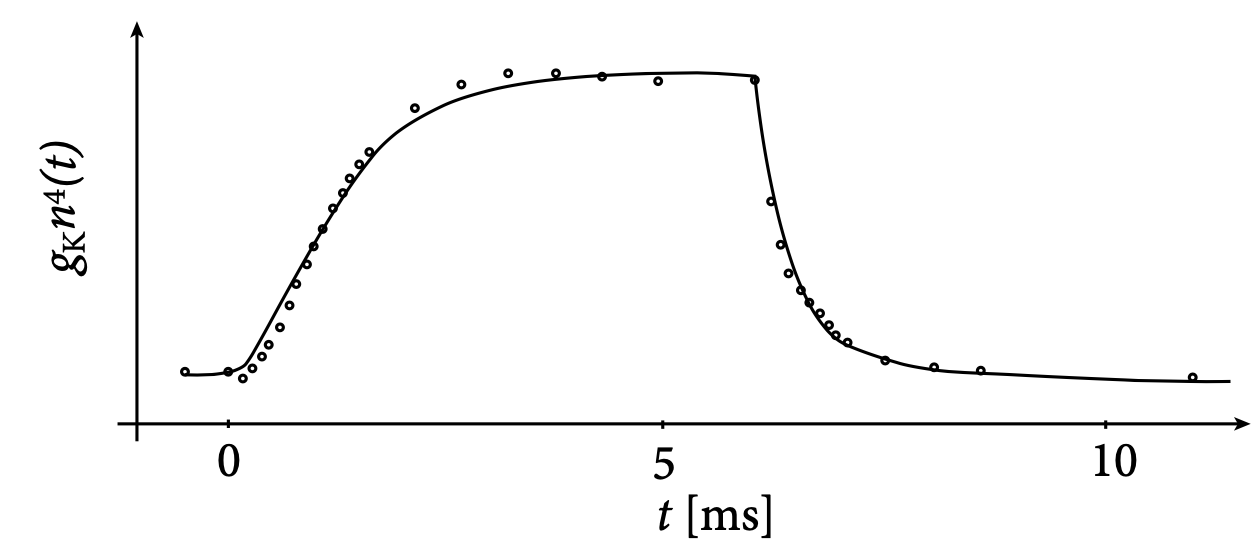
\includegraphics[width=13cm]{hodgkin_huxley_experiments}
	\caption{Experimental measurements (dots) and predictions of Hodgkin-Huxley model  (line). The horizontal axis represents time, the vertical is the electric potential of potassium ions.}
	\label{fig:hodgkin_huxley_experiments}
\end{figure} 

Hodgkin and Huxley have reduced the neuron into a simple electric circuit. Fluids inside the cell body are insulated from the outside environment by a membrane, which acts as a capacitor. It can store certain charge $q$ in form of ions such as $\ch{K+}$, $\ch{Na+}$, $\ch{Cl-}$. Let $n(x_1)$ and $n(x_2)$ denote the concentration of ions inside and outside the cell body, respectively. We can interpret $n(x)$ as proportional to the probability of finding an ion at point $x$ in space. From thermodynamics, we know that 
$n(x)\propto \exp(\frac{-E(x)}{kT})$, 
where $E(x)$ is the energy at a location $x$, $T$ is temperature and $k$ is the Boltzmann constant. Here, the energy is given by $E(x)=q u(x)$ for some electric potential $u(x)$ at point $x$. Therefore, we obtain
\[
\frac{n(x_1)}{n(x_2)} = \exp\big(-\frac{qu(x_1)-qu(x_2)}{kT}\big)
\]
The difference in electrical potential $\Delta u = u(x_1) - u(x_2)$ leads to  difference in ionic concentration and vice versa. This equation will hold true at the state of equilibrium. Solving for $\Delta u$ we can derive the Nernst equation 
\[
\Delta u = \frac{kT}{q}\ln\frac{n(x_1)}{n(x_2)}
\]
which determines the voltage of the system at equilibrium, given some difference in ion concentration. 
 
For example, it has been experimentally estimated that concentration of $\ch{K+}$ is approximately $\SI{140}{\milli\molar}$ inside the cell  and  $\SI{5}{\milli\molar}$ outside. Potassium has charge $q=\SI{1.6e-19}{\coulomb}$. Applying it to the formula with $k=\SI{1.4e-23}{\joule/\kelvin}$ yields Nernst potential of $E_{\ch{K}}=\SI{-83}{\milli\volt}$ at equilibrium. If the membrane potential $\Delta u$ falls below $E_{\ch{K}}$ (for example when an experimenter artificially injects current), the ions from outside will rush into the cell through ion channels in an effort to restore the equilibrium. When $\Delta u$ is above $E_{\ch{K}}$, the opposite happens. Hence, $E_{\ch{K}}$ is called the \textit{reversal potential}, as it causes the direction of current flow to reverse.

While the above derivation is concerned only with potassium ions, in reality there are many types of ions all contributing to membrane potential at the same time. When taken together, the true resting potential of a neuron is around $u_{rest} \approx \SI{65}{\milli\volt}$.

The cell membrane is a nearly perfect insulator, which acts as a capacitor. The only way for ions to cross it, is through the many gates (ion pumps and channels) on its surface.  Whenever a current $I(t)$ is  injected, it may either stay inside and charge the capacitor $C$, or leak outside through open channels with certain resistance. Hodgkin and Huxley model three types of channels. One selective only to sodium ions, one to potassium, and one unspecific that allows everything else to pass. They have their respective resistances $R_{\ch{Na}}$, $R_{\ch{K}}$ and $R_{\ch{L}}$. The final circuit schematic is presented on fig. \ref{fig:hodgkin_huxley_model}.
\begin{figure}[!htbp]
	\centering
	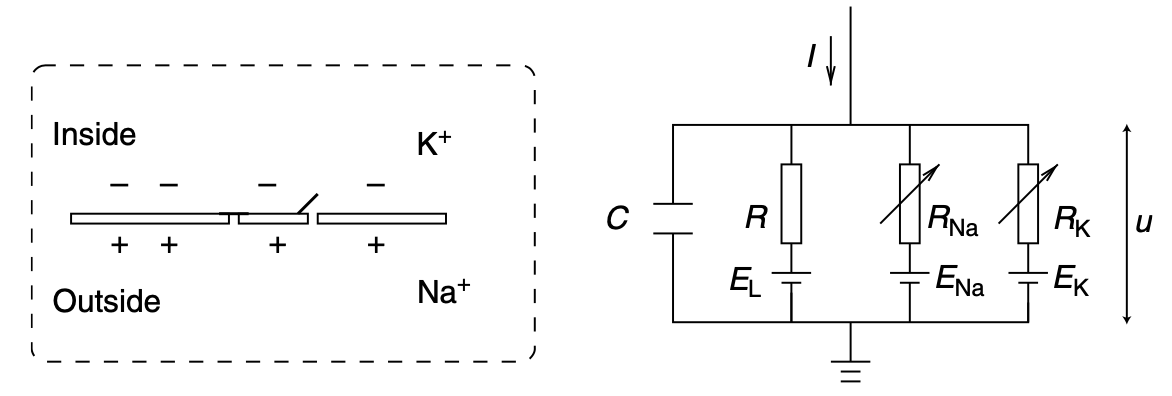
\includegraphics[width=13cm]{hodgkin_huxley_model}
	\caption{Schematic diagram of  Hodgkin-Huxley model}
	\label{fig:hodgkin_huxley_model}
\end{figure} 
By the conservation law of electric charge, we can split $I(t)$ into capacitive current $I_C$ and three other $I_{\ch{Na}}$, $I_{\ch{K}}$, $I_{\ch{L}}$ passing through each channel type.
\[
I(t) = I_C + I_{\ch{Na}} + I_{\ch{K}} + I_{\ch{L}}
\]
From the definition of capacity $C=\frac{q}{u}$ we get $I_C=C\frac{du}{dt}$.
\[
C \frac{du}{dt} = I(t) - I_{\ch{Na}} - I_{\ch{K}} - I_{\ch{L}}
\]
The voltage at the resistor $R_L$ (fig. \ref{fig:hodgkin_huxley_model}) is $u-E_L$, because $u$ is the total voltage and $E_L$ can be treated like a battery. From Ohm's law we obtain $I_L = \frac{u-E_L}{R_L}$. The denominator can be reformulated as conductance $g_L = \frac{1}{R_L}$. The current across all other channels can be derived analogously, except that potassium and sodium channels may sometimes be closed. To account for that, we need to multiply $ I_{\ch{Na}}$, $I_{\ch{K}} $ by some scalar representing what fraction of the channels are open at any point in time. The final Hodgkin-Huxley model is 
\[
C \frac{du}{dt}  = I(t) - g_{Na}m^3h(u-E_{Na}) - g_{K}n^4(u-E_{K}) - g_{L}m^3h(u-E_{L})
\]
where $m$ describes opening of sodium channels, $h$ represents their closing and $n$ is the activation of potassium channels. Those variables as well as their exponents have been deduced experimentally. Each one evolves according to its own differential equation. 

Integration of such equations allows us to simulate biological neurons with high degree of precision.

\subsubsection{Leaky integrate-and-fire model}

There exist many variations of the Hodgkin-Huxley model that account for more intricate biological details such as other ions, cable properties, compartmental structure of dendritic tree and so on. Such extensions come at a certain computational cost during simulation.

For our purpose of building artificial intelligence, the biological realism is of secondary importance. We are interested in abstracting away as much biophysics as possible, while still retaining the computational and algorithmic properties of neurons. One of such useful abstractions is the integrate-and-fire model.

It has been observed that the potential propagated through the membrane after stimulation is very noisy \cite{neuronal_dynamics} (fig. \ref{fig:membrane_potential_spike}), due to inherent randomness in closing and opening of ions channels. 
\begin{figure}[!htbp]
	\centering
	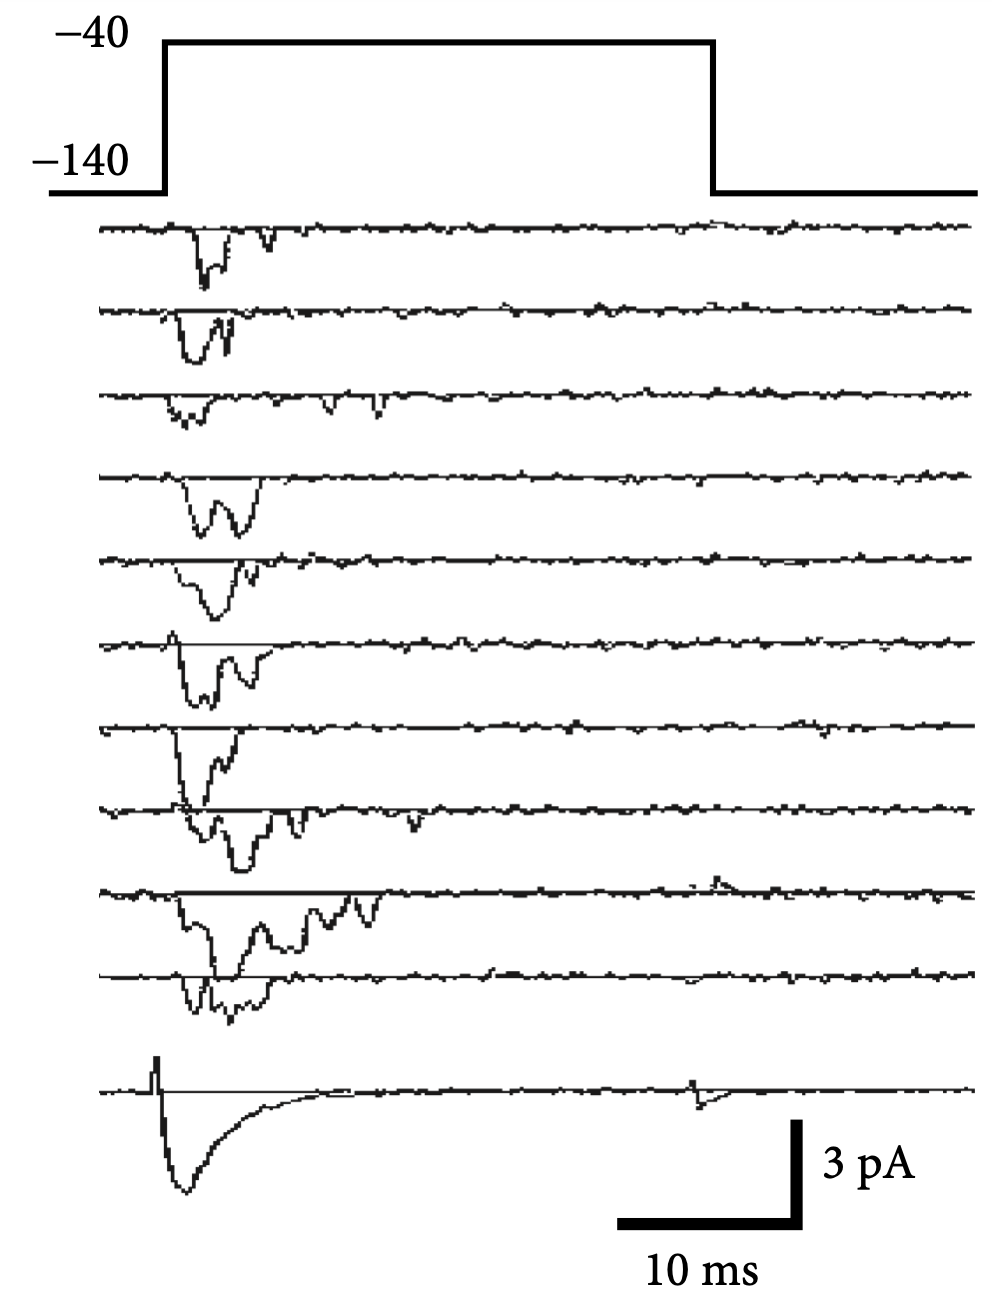
\includegraphics[width=5cm]{membrane_potential_spike}
	\caption{Current flowing through membrane after application of a voltage step (top row) over many trials. The bottom row presents the averaged response.}
	\label{fig:membrane_potential_spike}
\end{figure} 
The shape of action potentials generated at the soma is also unreliable and could not be used to effectively carry any information. Rather, it is believed that each spike carries only binary signal - either the neuron fired or it didn't. The shape and amplitude of a spike are not significant.

We can formally assume that a neuron will fire at time $t=t^f$, if the voltage $u(t^f)$ at the soma reaches a certain threshold $u(t^f)=\theta_{reset}$. When this happens, we reset the potential to some constant $u_r$ and then continue the integration of differential equations. Such instantaneous change can be expressed mathematically using delta functions $\delta(t-t^f)$. 

In general, an integrate-and-fire neuron evolves according to the equation
\[
\tau \frac{d}{dt}u = f(u) + R(u)I
\]
where $f$ is some function. One example is the standard leaky integrate-and-fire neuron, given by
\[
\tau \frac{d}{dt}u = -(u-u_{rest}) + R I
\]
The spikes produced by such models can be summed together to produce the spike train $S(t)=\sum_f \delta(t-t^f)$. The biological neurons are capable of generating such spike trains in a great variety of firing patterns (fig. \ref{fig:cortial_spike_patterns}).
\begin{figure}[!htbp]
	\centering
	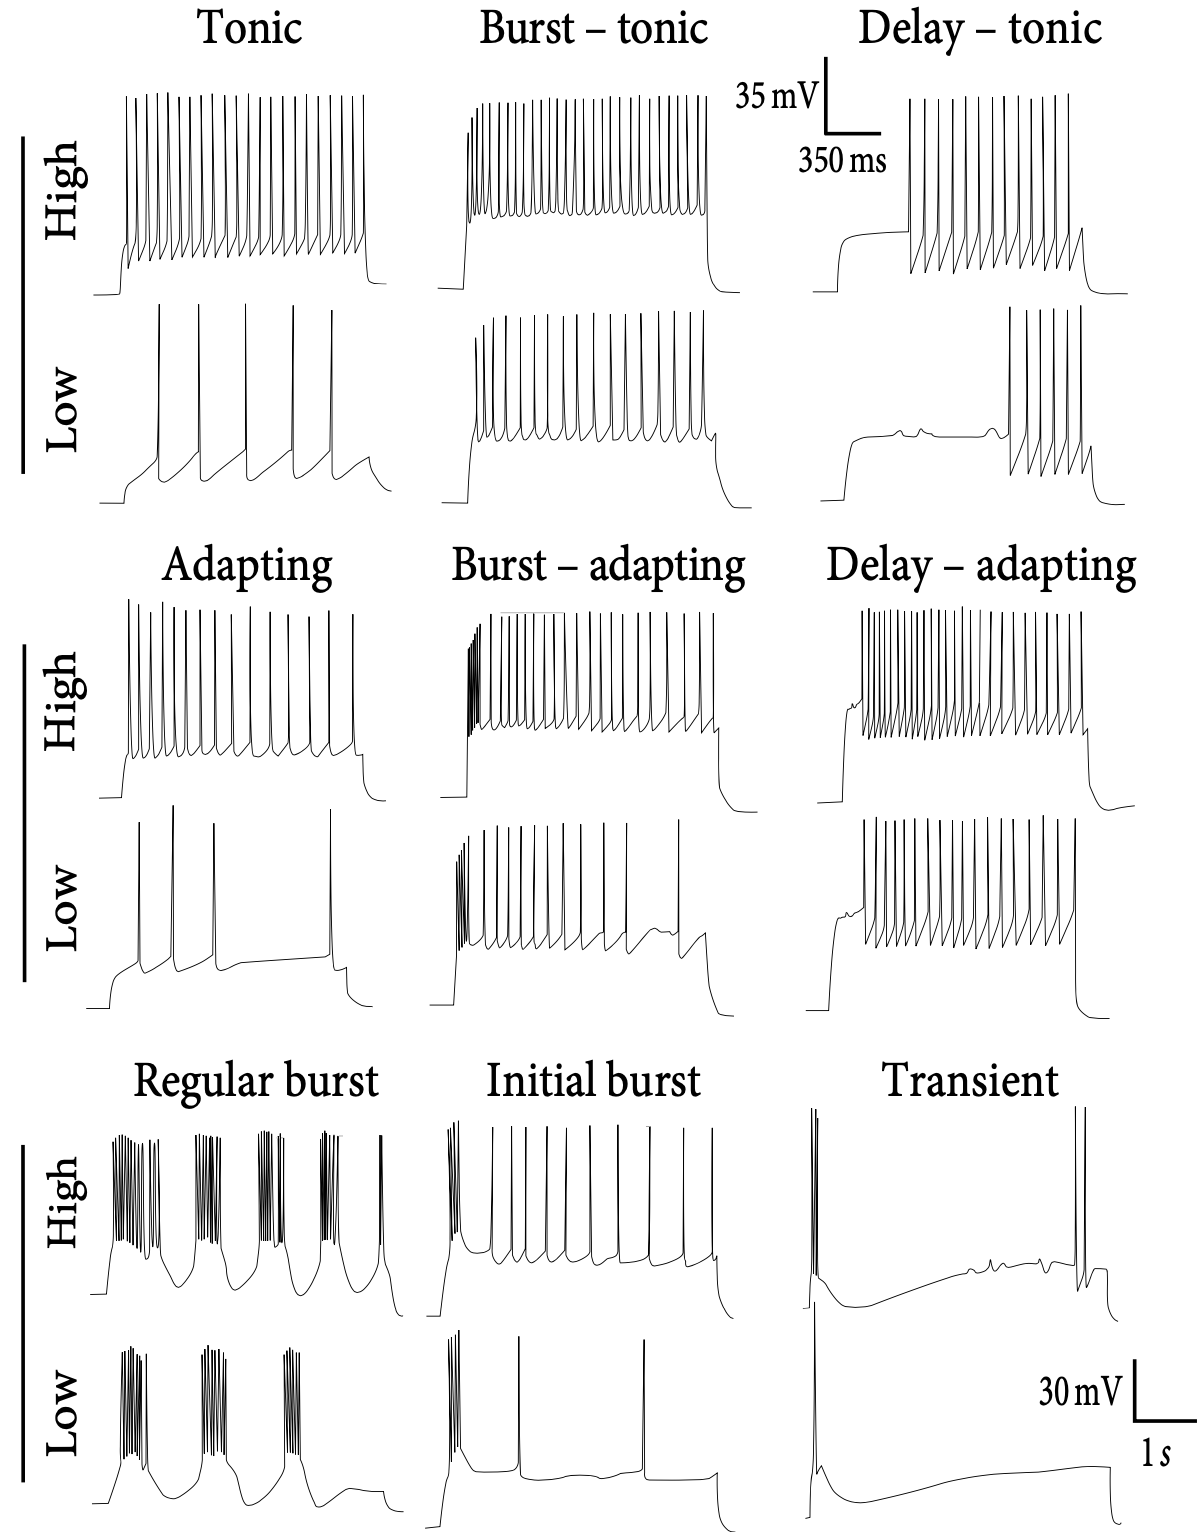
\includegraphics[width=13cm]{cortial_spike_patterns}
	\caption{Firing patterns observed in cortical neurons}
	\label{fig:cortial_spike_patterns}
\end{figure}
Neuroscientists have been able to reproduce all of these patterns using fire-and-integrate neurons such as AdEx or Izhikevich models.

\subsubsection{Spike response model}

So far, we've modelled the evolution of membrane potential $u$ using differential equations. It is possible to take a different approach and model $u$ as a convolution of the external input current $I_{ext}$ and a voltage response function $\kappa$.
\[
u_{stimulus}(t) = \int_{0}^{\infty} \kappa(\tau) I_{ext} (t-\tau) d\tau
\]
Such equation corresponds to the ``integrate'' part of an integrate-and-fire model. The effects of spike after-potential - the negative overshoot that typically occurs after a neuron fires (or as we know it, resetting $u$ to $u_r$ after reaching threshold $u_{reset}$) - can be modelled as another convolution of the produced spike train $S(t)$ with some function $\eta$
\[
u_{spike}(t) = \int_{0}^{\infty} \eta(\tau) S (t-\tau) d\tau
\]
By combining the two together and adding some bias term $u_{rest}$ we arrive at the definition of stimulus-response model (SRM)
\[
u(t) = \int_{0}^{\infty} \eta(\tau) S (t-\tau) d\tau + \int_{0}^{\infty} \kappa(\tau) I_{ext} (t-\tau) d\tau + u_{rest}
\]
The neuron fires  at time $t=t^f$ if the potential reaches some threshold $u(t)=u_{reset}$ from below, that is $\frac{du}{dt}>0$.



\subsubsection{Firing rate and temporal models}

There are plentiful ways of defining the firing rate for biological neurons. 
One of them is peri-stimulus-time-histogram (PSTH). An experimenter can perform many trials in vitro, stimulating the same neuron with the same current pattern several times, count the number of spikes and then calculate the average over trials. In nature, it is impossible for an animal to replay the same event in order to make such estimation, so a different alternative would be to take a large population of similarly connected neurons and then divide the number of spikes by the number of neurons. The approach that has the most similarity to SRM is to convolve the spike train $S(t)$ with some density function, and in this way approximate the instantaneous mean firing rate. 

The firing rate models have been extensively used as a basis for many machine learning models, including predictive coding and deep neural networks. Nonetheless, there exists significant experimental evidence against rate-based models. A fly can react to new stimuli and change the direction of flight within 30-40ms (Rieke et al., 1997). The concept of a firing rate does not have any meaning on such a small timescale, as it is impossible to count enough spikes to make any good estimation. Temporal averaging is only possible in scenarios where the stimulus is stationary, which is rarely the case in a natural environment.

A much more biologically plausible candidate is the so-called \textit{temporal coding}.
It assumes that the information is carried by relative timing of spikes. It doesn't matter how many action potentials arrive, but rather when they arrive relative to each other. In particular, we can imagine a scenario where some neuronal population is driven by an abrupt onset of stimulus. \textit{Latency code} assumes that  only the time (latency) of the first spike carries all the information. Consecutive spikes can be ignored. Within a population, one ``winning'' neuron can even cause activation of fast-spiking inhibitory interneurons, which prevent many of the slower excitatory neighbours from firing. This forms the basis of  winner-takes-all models. Instead of only limiting ourselves to a single abrupt stimulus event, the latency code can be extended to periodic input (fig. \ref{fig:phase_coding}a), driven by some background oscillation (such as brainwaves). In reality, most of the stimulus is continuous but not periodic, and several neurons often fire in a highly correlated patterns. Hence, it becomes possible to group several spikes together based on their temporal correlation and measure their latency relative to each other. This leads to the models of spike synchrony (fig. \ref{fig:phase_coding}b).
\begin{figure}[!htbp]
	\centering
	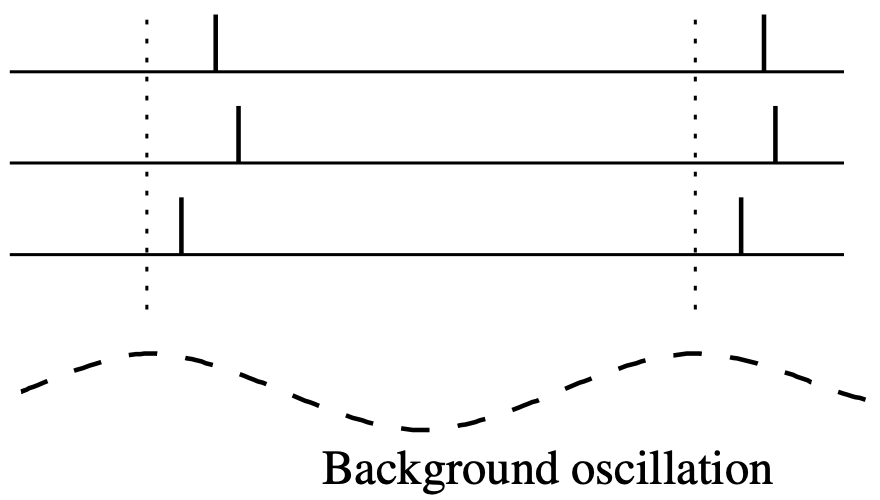
\includegraphics[width=5cm]{phase coding}
	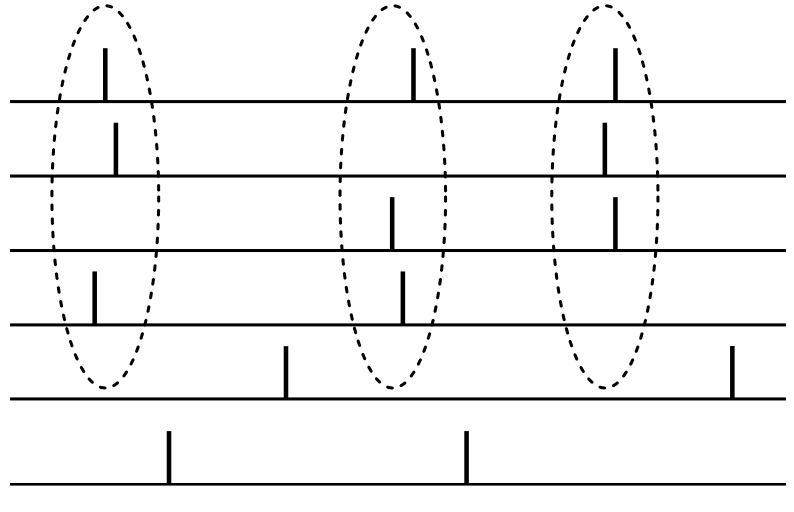
\includegraphics[width=5cm]{synchrony}
	\caption{(a) Phase coding measures the time of the first spike, relative to some background oscillation. (b) Synchrony of neuron spikes means that several neurons often fire closely together. The first spike within the synchronous group, matters the most.}
	\label{fig:phase_coding}
\end{figure}

Having briefly introduced rate-coding and temporal-coding, we can explain the connection between all of them and show that sometimes, the line between rate and relative timing is blurry.

In PSTH, we tried to estimate firing rate after an onset of a known stimulus. Now we consider the opposite scenario, where we  try to estimate the average stimulus that needs to arrive before a specific neuron fires (fig. \ref{fig:reverse_correlation}). This is called the \textit{reverse correlation}.
\begin{figure}[!htbp]
	\centering
	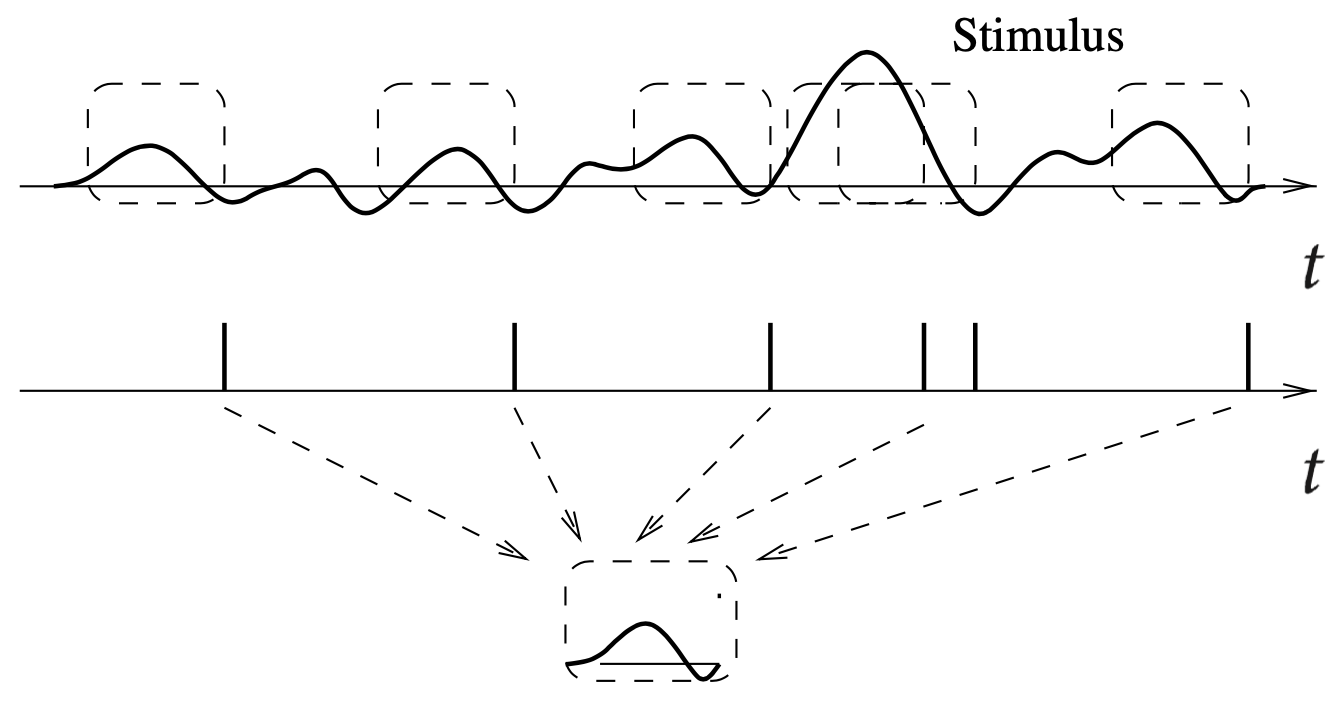
\includegraphics[width=9cm]{reverse_correlation}
	\caption{For every spike, we take a short window of the preceding signal. Then we average the windows to estimate the ``typical'' stimulus for a given neuron.}
	\label{fig:reverse_correlation}
\end{figure}
Formally, let $I(t)$ be some stimulus received by a neuron. For every spike at time $t^f$, we take a short time window $\kappa(t-t^f)$ of the stimulus and sum over all spikes $I_{estimte}(t)=\sum_f \kappa(t-t^f)$. The kernel $\kappa$ is a function that characterizes ``receptive field'' of a neuron. It is a signal that leads to the greatest excitation and minimizes the error $\int \big(I(t)-I_{estimate}(t)\big)^2dt$. By fitting optimal $\kappa$ to experimental data, it is not only possible to predict future activations, but also accurately reconstruct stimulus from the observed spike trains (fig. \ref{fig:reverse_correlation_estimate}).
\begin{figure}[!htbp]
	\centering
	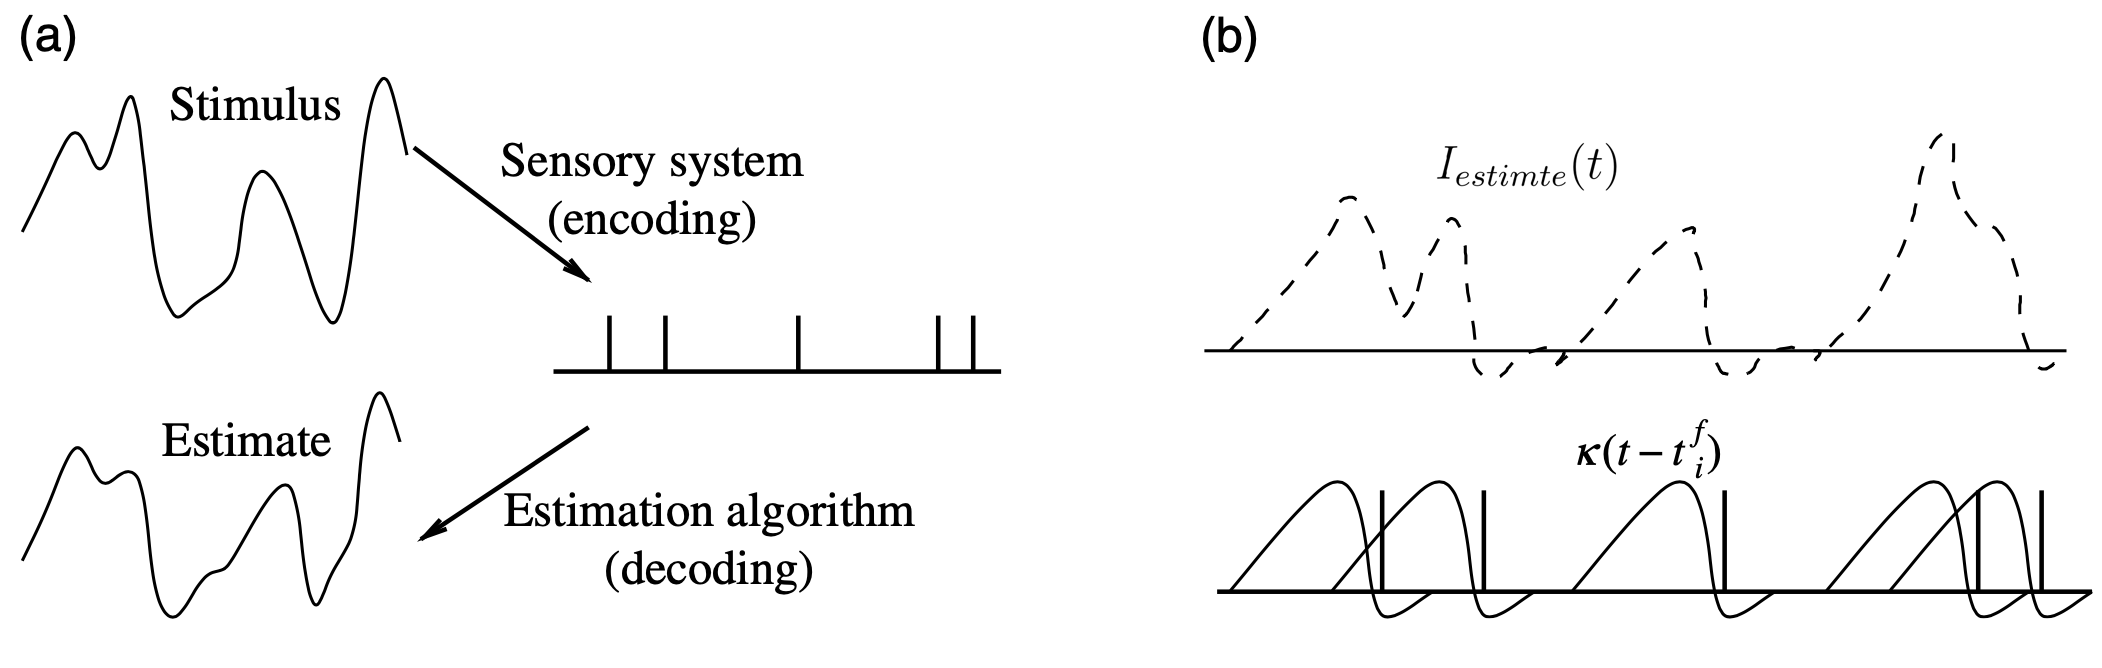
\includegraphics[width=13cm]{reverse_correlation_estimate}
	\caption{(a)  An unknown stimulus evokes a spike train. Knowing the right kernel function, it is possible to reconstruct the original signal. (b) Linear reconstruction of stimulus is achieved by summing the same kernel at each spike time.}
	\label{fig:reverse_correlation_estimate}
\end{figure}

Reverse correlation may seem like a generalization of latency coding. At the same time, it can be used to define instantaneous firing rate $r$
\[
r(t) = \frac{\int \kappa(\tau) S(t-\tau)d\tau}{\int \kappa(\tau) d\tau}
\]
When $r$ is high, the neuron will be more likely to fire first and inhibit others. When $r$ is low, the neuron is expected to fire late. Thus, firing rate carries a lot of information about latency of first spike and vice versa.

\subsection{Geometric deep learning theory}

Neuroscientific models can tell us a lot about the functioning of biological neurons, but their practical applications have been limited. As of today, deep learning remains the only tool capable of producing end results that resemble complex intelligent behaviour.
The success of deep networks can be largely attributed to their ability of expressing algebraic symmetries in the data. This notion is studied and formalized by geometric deep learning theory \cite{geom_deep_learn}.

\subsubsection{Curse of dimensionality}

Let us consider a set of \textit{i.i.d.} observed samples $\mathcal{D}=\{(x_i,y_i)\}_{i=1}^N$ drawn from some distribution $P$ defined over domain $\mathcal{X}\times \mathcal{Y}$. We assume existence of some unknown function $f:\mathcal{X}\rightarrow\mathcal{Y}$ such that $f(x_i)=y_i$ for all $i=1...N$. Learning is defined as the problem of identifying $\tilde{f}$ from a parametric family $\mathcal{F}=\{f_{\theta\in\Theta}\}$ such that $\tilde{f}(x_i)=f(x_i)$ for all $i=1...N$. In the case of deep learning, the set of parameters $\Theta$ corresponds to network weights. The expected performance  of $\tilde{f}$ is defined as 
\[
R(\tilde{f})=\mathbb{E}_{P} L(\tilde{f}(x),f(x))
\]
where $L$ is some loss function. $R$ can be estimated by drawing new unseen samples $(x_i,y_i)$ for $i>N$.

For low-dimensional functions, learning can be achieved with classical techniques of statistics. As dimensionality increases, the number of samples $N$  necessary to correctly identify $\tilde{f}$, grows exponentially and learning becomes infeasible. This phenomenon, known as \textit{curse of dimensionality}, can be proved as follows.

Suppose $f: \mathbb{R}^d\rightarrow\mathbb{R}$ is 1-Lipschitz continuous, i.e. satisfies $\vert f(x)-f(x')\vert \le \lVert x-x'\rVert$. We can devise a simple yet pessimistic scenario $f(x)=\sum_{j=1}^{2^d} z_j \phi(x-x_j)$ where $z_j=\pm 1$, $x_j\in R^d$ is placed in each quadrant, and $\phi$ is a locally supported Lipschitz ``bump'' (fig. \ref{fig:curse_of_dim}).
\begin{figure}[!htbp]
	\centering
	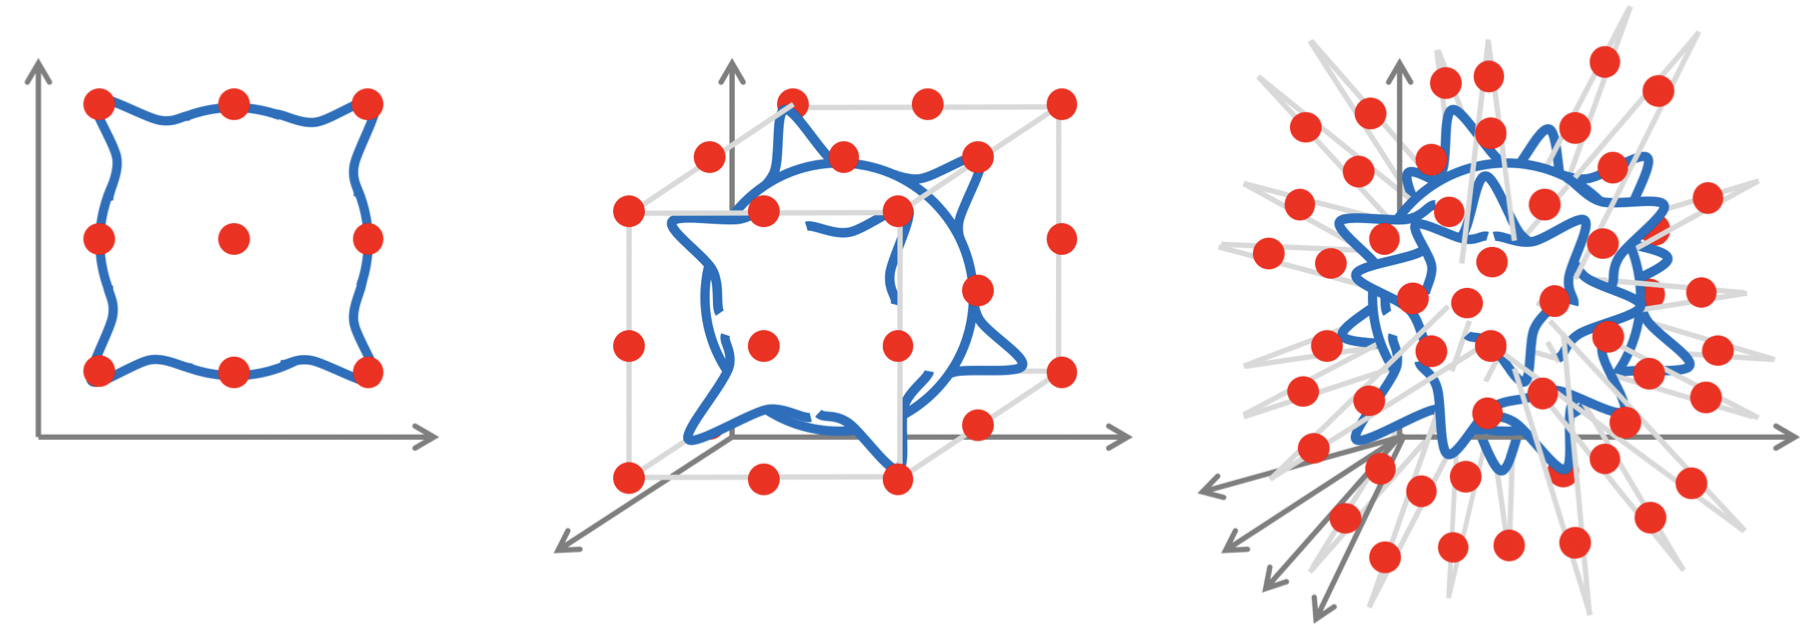
\includegraphics[width=13cm]{curse_of_dim }
	\caption{Illustration of $f(x)=\sum_{j=1}^{2^d} z_j \phi(x-x_j)$ in higher dimensions $d$.}
	\label{fig:curse_of_dim}
\end{figure}
In order to identify $f$ we have to observe each one of the ``bumps''. Therefore, $N$ must grow exponentially $2^d$ with dimensionality $d$. This argument can be fully formalized using the notion of maximum discrepancy \cite{lipschitz}.

\subsubsection{Geometric priors}

If we could capture symmetries of the function $f$ and narrow down the search space $F$, learning in higher dimensions would become easier. To formalize such geometric priors, we assume that $\mathcal{X}$ is a space of signals (functions)
\[
\mathcal{X} = \Omega \rightarrow \mathcal{C}
\]
where $\Omega$ is some domain and $\mathcal{C}$ is a vector space called \textit{channels}. Such $\mathcal{X}$ is itself a vector space, because we can define addition and scalar multiplication of signals
\[
(\alpha x + \beta x')(u) = \alpha x(u) + \beta x'(u) \text{ for all }u \in \Omega
\]
Given an inner product $\langle c,c' \rangle$ on $\mathcal{C}$ and measure $\mu$ on $\Omega$, we can define inner product
\[
\langle x,x' \rangle = \int_{\Omega} \langle x(u),x'(u) \rangle d \mu(u)
\]
making $\mathcal{X}$ a Hilbert Space.

A typical example might be RGB images of $n\times n$ pixels. The domain could define pixel coordinates $\Omega = \mathbb{Z}_n \times \mathbb{Z}_n$ and channels $\mathcal{C}=\mathbb{R}^3$ could be the colour values. An image $x$ is a function that takes as input coordinates of a pixel and returns the corresponding vector of RGB values.

Geometric priors can be defined as algebraic symmetries. A symmetry of an object determines its invariance to certain transformations. For example, rotating a square by $90^\circ$ does not result in any change. A set of transformations constitutes a group $G$. Elements $g,g'$ of $G$ can be composed together, which we denote as $gg'$. For instance, let $g$ be clockwise rotation by $90^\circ$ and $g'$ be counter-clockwise rotation by $90^\circ$, then their composition $gg'$ results in $0^\circ$ (no rotation). 

Group elements can be composed together, but they may also act on other sets. In particular, $g\in G$ could act on $u\in \Omega$ denoted as $u.g$. For example, let $G$ be the group of 2-dimensional translations and $\Omega=\mathbb{Z} \times \mathbb{Z}$ be the set of points. If $g$ is the transformation of ``moving 3 steps left, 2 steps up'' and $u$ is a point $(3,5)$ then $u.g$ yields a new point $(0,7)$.

If $G$ acts on domain $\Omega$, then we can naturally define $G$'s action on signal $\mathcal{X}$
\[
x(u).g = x(u.g)\text{ for all }g\in G
\]
Symmetries may not only be exhibited by sets, but also by functions. We say that $f:\mathcal{X}\rightarrow\mathcal{Y}$ is $G$-invariant when $G$ acts on $\mathcal{X}$ and 
\[
f(x.g) = f(x)\text{ for all }g\in G
\]
If $G$ also acts on $\mathcal{Y}$, then we can introduce  $G$-equivariance as
\[
f(x.g) = f(x).g \text{ for all }g\in G
\]  
Deep learning architectures give us means of expressing geometric priors by constraining network layers (functions) to being invariant or equivariant with respect to some $G$. For example the convolutional neural networks enforce shift-equivariance to 2D translations. Transformers express permutation-equivariance. LSTMs and RNNs use time-warping.


\subsection{Reinforcement learning}

Let us now consider  the problem of learning to interact with a dynamic environment. It is a very different scenario from the classic problem of fitting functions to a static dataset of samples. Thus, a different framework is necessary to describe such type of intelligence.

\subsubsection{Markov decision processes}

Reinforcement learning \cite{rl_sutton} is based on the interplay between agent and environment. 
It is mathematically formalized as a \textit{Markov decision process} (MDP).
At time-step $t$ the agent is in some state $S_t$ of the environment. The agent can take an action $A_t$, which results in transition to a new state  $S_{t+1}$ (fig. \ref{fig:agent_env_interaction}). 
\begin{figure}[!htbp]
	\centering
	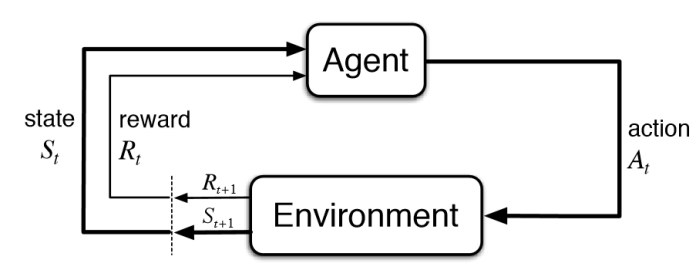
\includegraphics[width=13cm]{supervised reinforcement learning}
	\caption{Agent-environment interaction}
	\label{fig:agent_env_interaction}
\end{figure}
At each step, the agent receives some reward $R_{t+1}$. This process can be repeated, producing a sequence of states, actions and rewards
\[
S_0, A_0, R_1, S_1, A_1, R_2, S_2, R_3 ...
\]
Such sequence is known as a \textit{trajectory}. The transition between environment states is defined by a \textit{dynamics function} $p:S\times R\times S \times A \rightarrow [0,1]$
\[
p(s',r | s, a)
\]
It specifies the probability of transitioning to state $s'$ and receiving reward $r$ after taking action $a$ in state $s$. Reward $r$ is typically assumed to be some real number. If we ignored the actions and rewards, we would obtain a transition function  $p:S\times S \rightarrow [0,1]$, which is the classical definition of a  Markov chain. 

MDP formalizes behaviour of an agent using \textit{policy function} $\pi:A\times S\rightarrow[0,1]$
\[
\pi(a|s)
\]
In order to randomly sample trajectories, both $p$ and $\pi$ are necessary. 
\[
p_{\pi}(s',r|s) = \sum_{a\in A}p(s',r|s,a)\pi(a|s)
\]
There are two possible regimes of sampling, depending on the kind of task. 
In the case of episodic tasks, the trajectory is always finite. It has a  \textit{terminal state} $S_T$ and the trajectory itself is referred to as an \textit{episode}. We can define \textit{return} as sum of rewards
\[
G_t = R_{t+1}+R_{t+2}+...R_T
\]
In the case of continuous tasks, the trajectory may be infinite and the agent might never halt. In order to provide a meaningful definition of return, a discount rate $\gamma$ is necessary 
\[
G_t = R_{t+1}+\gamma R_{t+2}+\gamma^2 R_{t+3}+...
\]
The expected return is defined as the expectation of $G$ when the trajectories are sampled according to distribution $p_\pi$.

\subsubsection{Bellman equations}
An intelligent agent should be able to plan its actions in such a way as to receive maximal possible reward with high probability. Therefore, the goal of reinforcement learning is formulated as maximization of expected return. A policy $\pi$ that maximizes $\mathbb{E}_\pi [G]$ is called \textit{optimal} and is denoted as $\pi_*$. One technique for finding $\pi_*$ is through the use of \textit{value function} $v$, defined as 
\[
v_\pi(s) = \mathbb{E}_\pi [G_t|S_t=s]
\]
which represents the reward an agent expects to receive if it finds itself in state $s$. Value function can be restated in a recursive form
\begin{equation}
	\begin{split}
		v_\pi(s) & = \mathbb{E}_\pi [G_t|S_t=s] \\
		& = \mathbb{E}_\pi [R_{t+1}+\gamma G_{t+1}|S_t=s] \\
		& = \sum_{s',r} p_\pi(s',r|s)(r+\gamma \mathbb{E}_\pi [G_{t+1}|S_{t+1}=s']) \\
		& = \sum_{s',r} p_\pi(s',r|s)(r+\gamma v_\pi(s')) \\
	\end{split}
\end{equation}
This is known as a Bellman equation. 
Optimal value function $v_*$ is one that would always choose the best policy in any state
\[
v_*(s) = \max_\pi v_\pi(s)\text{ for all }s\in S
\]
It also can be reformulated recursively, yielding the Bellman optimality equation
\begin{equation}
	\begin{split}
v_*(s) & = \max_a \mathbb{E}[R_{t+1}+\gamma v_*(S_{t+1})|S_t=s,A_t=a] \\
		& = \max_a  \sum_{s',r} p(s',r|s,a)(r+\gamma v_*(s')) \\
	\end{split}
\end{equation}
This defines a system of equations (one for each state $s$), which has a unique solution (if set $S$ is finite). For simple environment is it possible to solve $v_*$ analytically. If we have $v_*$, then $\pi_*$  can be easily obtained by greedily following $v_*$.
\[
\pi_*(s) = \argmax_a \sum_{s',r} p(s',r|s,a)(r+\gamma v_*(s')) 
\]
Despite the greediness, such $\pi_*$ is indeed  optimal in the long-term, because $v_*$ already accounts for all future rewards.

If the dynamics function $p$ is not known, or the environment is too large and complex to allow for direct solutions to $v_*$, then we can resort to use of dynamic programming. Let $V$ be our estimate of $v_\pi$, which we iteratively refine by leveraging the temporal difference algorithm
\[
V(S_{t}) \leftarrow V(S_{t}) + \alpha\big(R_{t+1}+\gamma V(S_{t+1}) - V(S_{t}) \big) 
\] 
This update rule is a direct consequence of Bellman equation. The difference $R_{t+1}+\gamma V(S_{t+1}) - V(S_{t})$ is known as temporal-difference error.
After sampling enough trajectories, $V$ should converge to $v_\pi$. Then we can bootstrap and use $V$ to determine a new better policy $\pi'$, which greedily chooses $a$ that maximizes $v_\pi$. This process can be repeated until both $V$ and $\pi$ converge to optimal $v_*$ and $\pi_*$ (fig. \ref{fig:policy_iteration}).
\begin{figure}[!htbp]
	\centering
	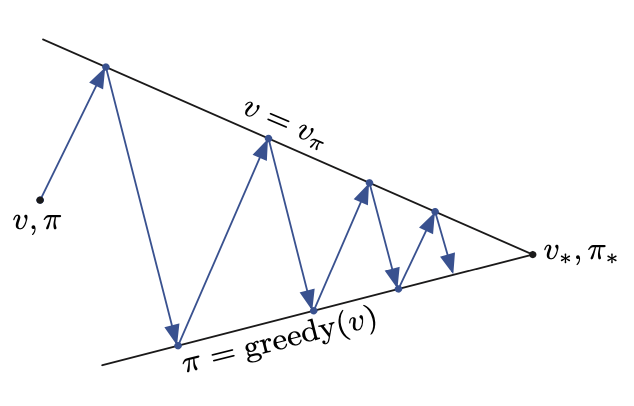
\includegraphics[width=7cm]{policy_iteration}
	\caption{Value iteration algorithm converges to optimal $v_*$ and $\pi_*$.}
	\label{fig:policy_iteration}
\end{figure}

\subsection{Cognitive maps and hippocampus modelling}

The theory of Markov decision processes gives us an elegant and abstract mathematical framework that can be applied to any control task. Does it mean that the real brains use a value function and temporal-difference learning?


\subsubsection{Tolman's experiments on rats}

In 1948, Edward Tolman published a collection of experiments investigating decision-making and planning in rats \cite{cog_maps_tolman}. One of them was the T-Alley Maze (fig. \ref{fig:tolman_maze}).
\begin{figure}[!htbp]
	\centering
	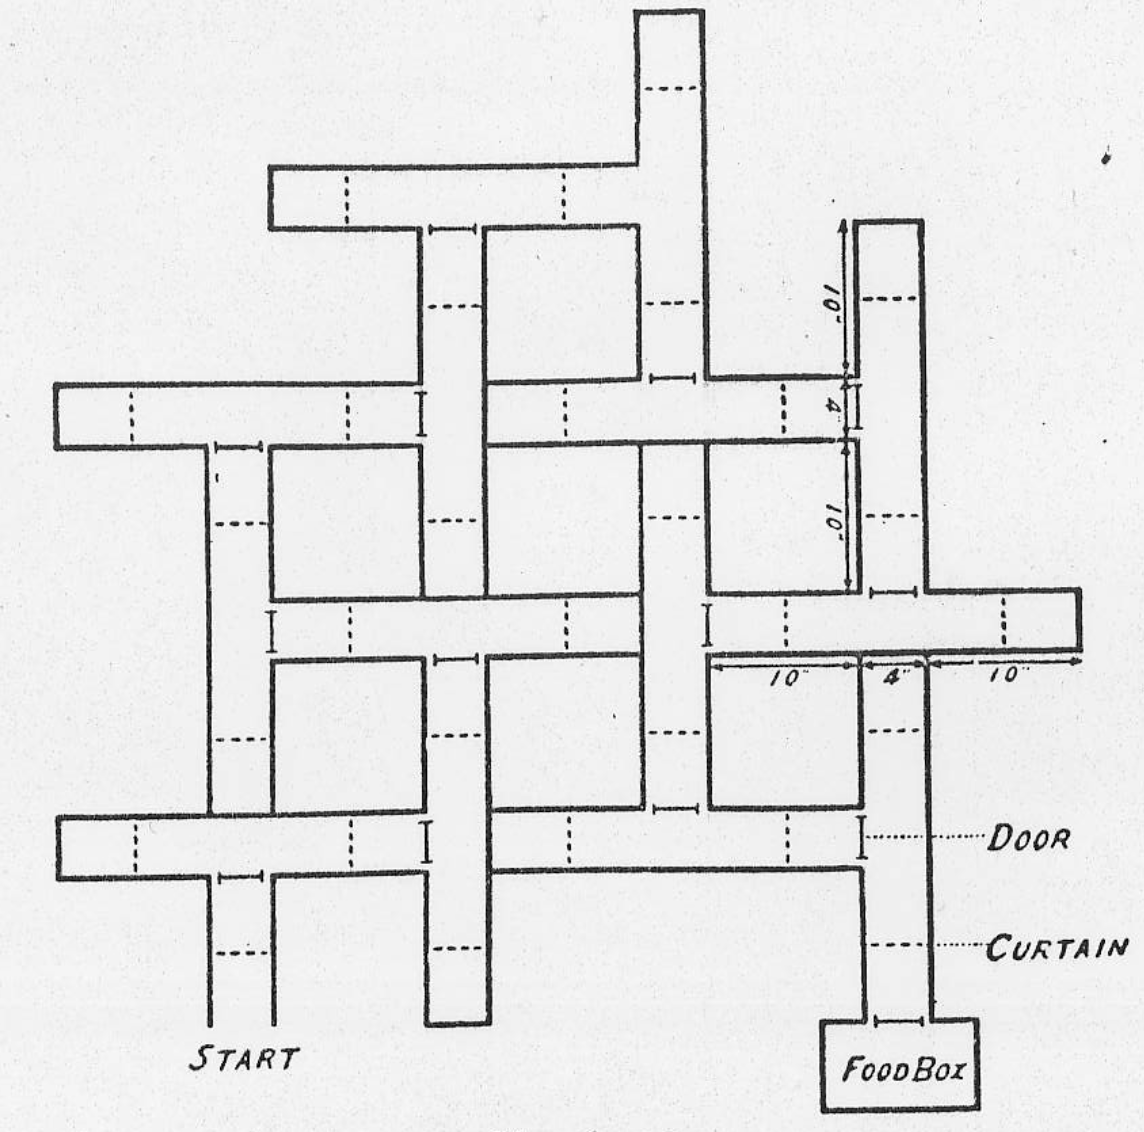
\includegraphics[width=9cm]{tolman_maze}
	\caption{Plan of the maze}
	\label{fig:tolman_maze}
\end{figure}
Animals would be placed inside the maze and allowed to wander. There were two control groups - one that never had food in the maze (HNR) and one that always did (HR). There was also a third group (HNR-R) that did not see any food at the beginning of experiment but then on 11th day and onwards it would be provided. Each rat would be let into the maze once a day. Experimenters would count the number of errors that rats made on their way to the food box. The results are presented on figure \ref{fig:tolman_maze_results}.
\begin{figure}[!htbp]
	\centering
	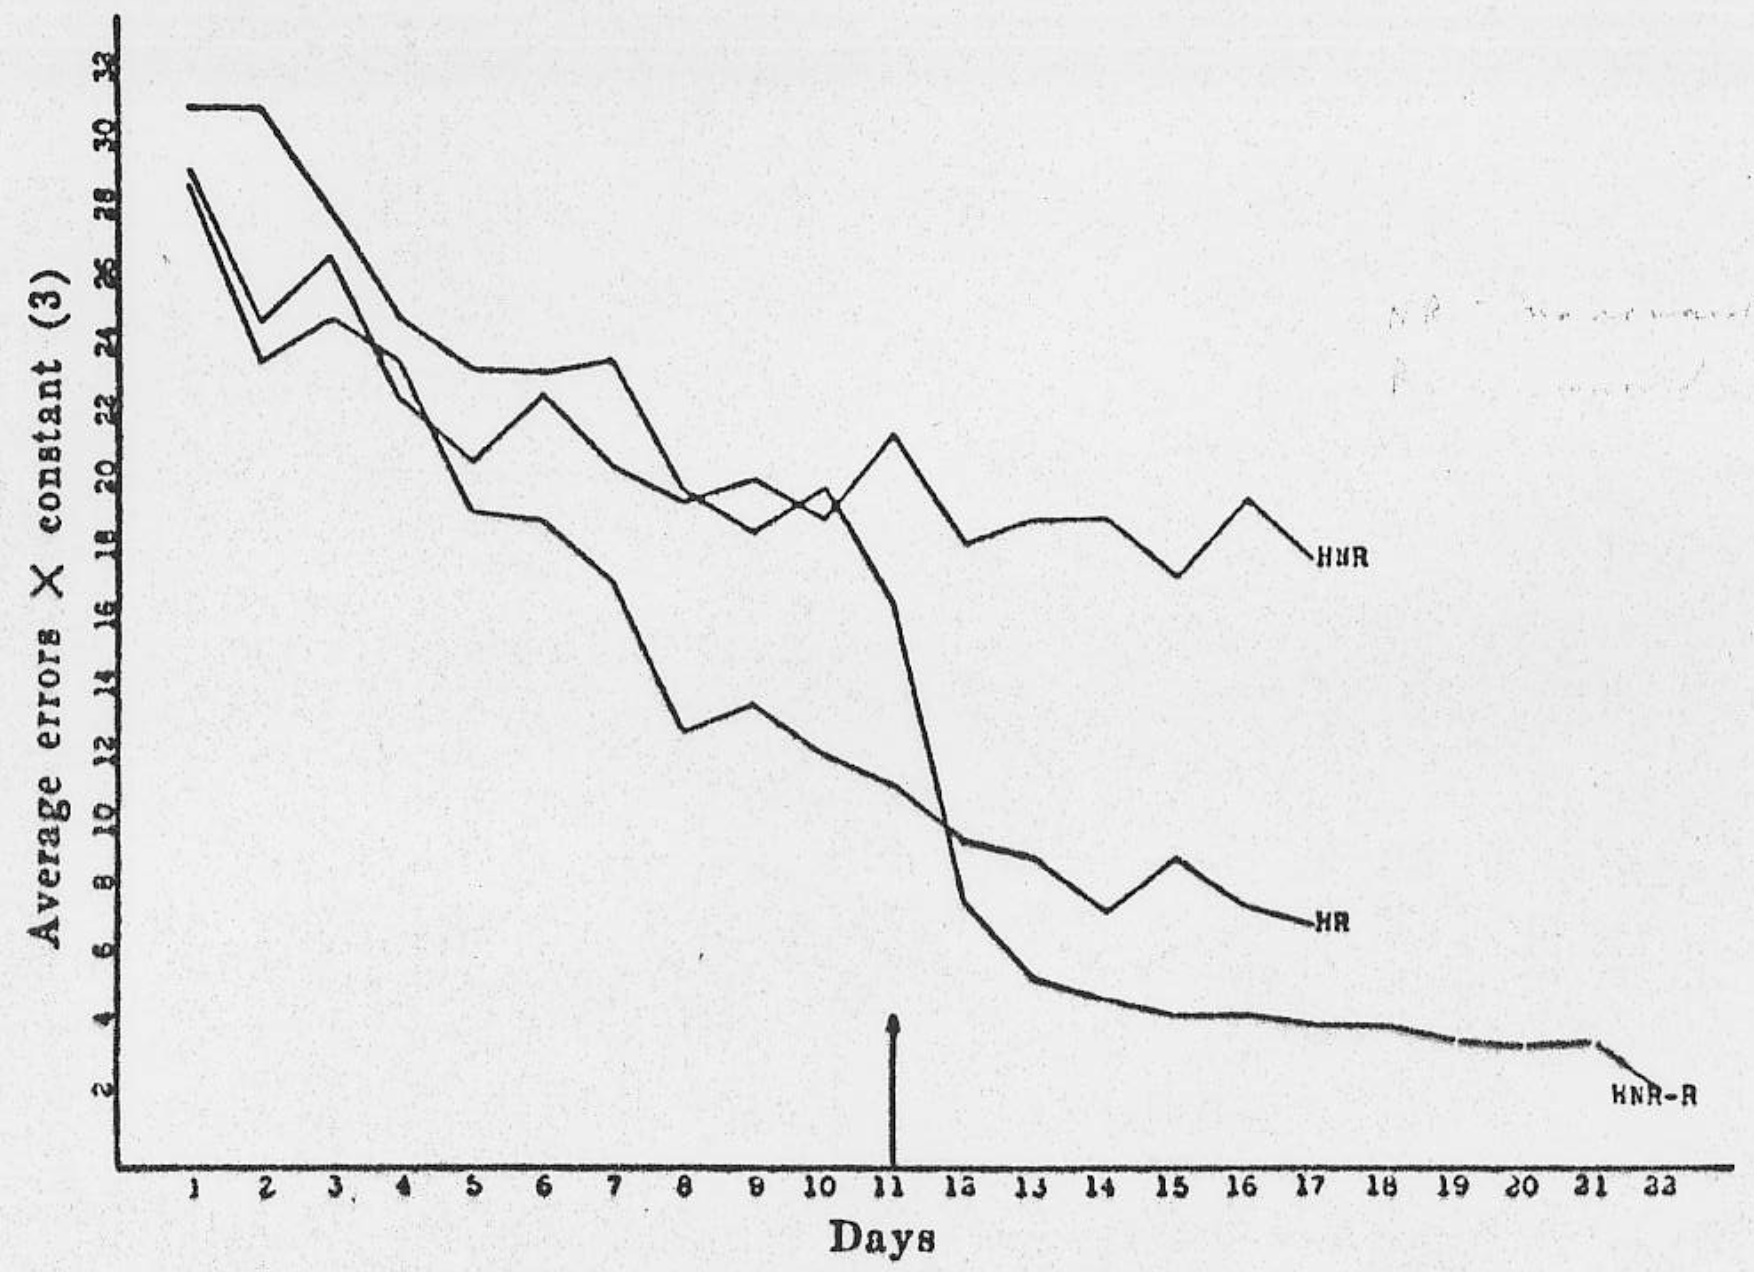
\includegraphics[width=9cm]{tolman_maze_results}
	\caption{Plan of the maze}
	\label{fig:tolman_maze_results}
\end{figure}
The most surprising finding occurred in group HNR-R. On the 12th day, experimenters observed a sudden drop in the error count, indicating that rats have already learned the structure of the maze, despite not receiving any reward for most of the experiment. This phenomenon has been termed \textit{latent learning} in the animal behaviourist literature. It is defined as any form of learning whose effects are not apparent during the course of learning, but can manifest themselves in a different scenario at some future time.

At the time of Tolman's publication, there existed two schools of thought trying to explain animal behaviour in different ways. The first group consisted of people claiming that animals are driven by mere \textit{stimulus-response} connections and reflexes. In their view, the environment would produce some (visual/auditory/tactile/...) signal that stimulates receptor neurons and the brain functions like a telephone relay, routing the stimulus to some endpoints responsible for muscle movement. In such framework, learning would be achieved by strengthening connections between those inputs and outputs that carried animal to reward. Analogically, if some sequences of outputs resulted in pain or other discomfort, then the connections to preceding inputs would be weakened.

The other group of psychologists claimed that the brain is more like a map. As the animal moves around and explores the environment, the brain relates consecutive places and experiences together, resulting in a graph of  connections resembling a map-like structure. Such type of learning can occur even in the absence of reward. At a later point in time, the animal can use its internal \textit{cognitive map} to plan ahead. 

I would like to point out a striking resemblance between stimulus-response theory and the modern deep reinforcement learning algorithms such as deep Q-learning. This approach has led to many success stories (AlphaGo, AlphaStar...). Does this mean that the biological brains should also use stimulus-response framework?

\subsubsection{Grid cells, place cells and the hippocampus}
Since the formulation of the cognitive map hypothesis, neuroscience has provided us with a plethora of evidence in its favour.

In 1971, John O'Keefe and Jonathan Dostrovsky performed one of the first experiments demonstrating the significance of hippocampus in spacial navigation \cite{OKEEFE1971171}. By placing electrodes in a rat's brain and measuring activity of neurons, they noticed that some of them would only fire whenever the  rat was in a specific place of the testing platform. These neurons were later termed as \textit{place cells}.

In 2005, Edvard Moser and May-Britt Moser, discovered neurons in medial entorhinal cortex that would respond whenever a rat was in one of several places \cite{Hafting2005}. When plotted in two dimensions, those places would be arranged in a hexagonal grid-like pattern. Such neurons have been termed as \textit{grid cells}. In 2014 both of those discoveries won a Nobel Prize in Physiology and Medicine. 

Another similar type of neurons are the \textit{head-direction cells} \cite{HD_cells}, which can be found in many brain areas. Their response becomes strongest whenever the animal's head is facing a specific direction. Grid, place and head-direction cells have been observed in many species, but the brains of primates have several unique features and neurons not found anywhere else. One of them are spacial-view cells, which activate whenever a primate is looking at a specific place. All these types of cells are summarized on figure  \ref{fig:place_grid_head_view_cells}.
\begin{figure}[!htbp]
	\centering
	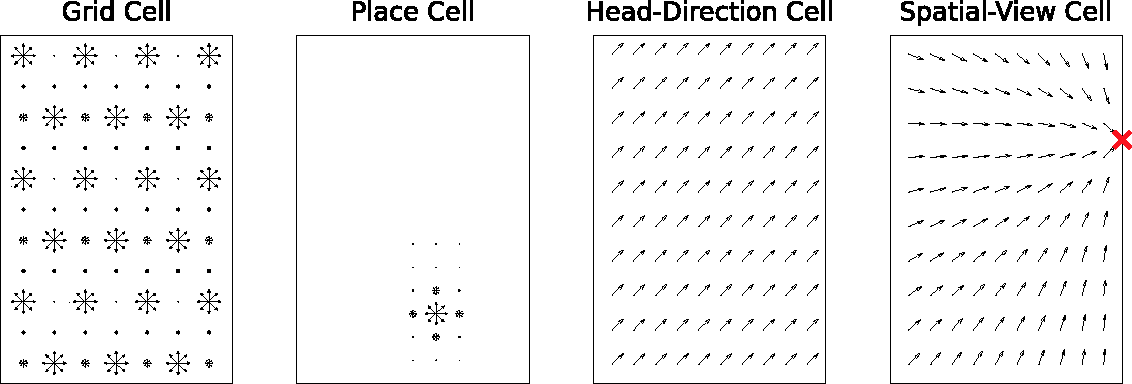
\includegraphics[width=12cm]{place_grid_head_view_cells}
	\caption{A schematic representing activations of different cell types. The location and direction of an arrow corresponds to the place and direction of a rat's head. Arrow length depicts the firing rate of a neuron. Figure from  Franzius, Sprekeler, Wiskott \cite{slowness_sparseness}.}
	\label{fig:place_grid_head_view_cells}
\end{figure}

Entorhinal cortex hosts boundary-vector cells \cite{BVC}, which fire whenever the animal finds itself in specific distance and orientation to some environmental boundary, such as walls, holes or impenetrable objects.  There are also many other types of object-vector cells, which fire in response to any object being located in a specific place relative to the agent \cite{vector_trace_cells}.

The activation patterns of grid cells are not always regular. The shape of the environment often has a significant influence on them. Krupic et al. \cite{Kurpic} has performed many experiments investigating this phenomenon (fig \ref{fig:kurpic}). The boundary-vector cells may also have an influence on grid and place cells \cite{boundary_vector_cells}.
\begin{figure}[!htbp]
	\centering
	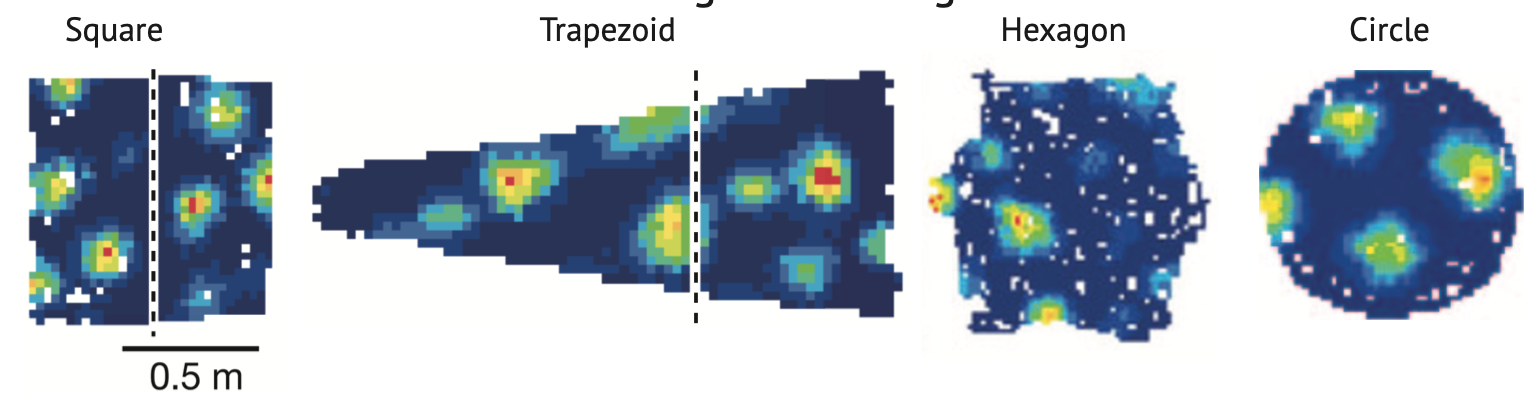
\includegraphics[width=12cm]{kurpic}
	\caption{Histograms showing the effect of compartment shape on the grid cell firing fields.}
	\label{fig:kurpic}
\end{figure}
Certain species of mammals, such as bats, can fly and their place and grid cells fire in three-dimensional patterns. An interesting finding was that even grounded animals, such as rats,
can exhibit three-dimensional activation patterns if placed in environments that allow climbing in all directions \cite{grid_cells_3d}. This suggests that mechanisms behind these neurons are general, flexible and adaptable to many situations.
It has been found that rat hippocampus contains cells that do not only code for location, but can represent sound frequencies (if trained that turning a lever to produce a specific pitch results in reward), counting (number of laps when moving in a circular track), logical dependencies between cues and rewards (moving left or right in a T-maze depending on what happens before), or potentially any abstract knowledge about the environment \cite{hippocampus_abstract_geometry}. 

Place cells do not only code for current location, but they can also fire in sequences that predict future paths that the rat will take \cite{place_cell_sequences}. For this reason, the hippocampus is thought to play an essential role in planning. This led to formulation of predictive map hypothesis, which states that the place cells do not code for current location, but rather predict the next state of the animal \cite{predictive_map}. After a rat traces some path and the corresponding place cells fire at each intermediate location, the same sequence of  neurons is then replayed again but in reverse order. This mechanism is called \textit{sharp-wave-ripple} and is thought to be important for formation of episodic memory \cite{shard_wave_ripple,alternating_sequences}. It is believed that planning into the future and remembering the past might reuse the same underlying mechanisms \cite{past_and_future}.  The generality of abstract knowledge represented in hippocampus is a sign that the mechanism responsible for emergence of place cells could be also used to explain higher cognitive functions in other parts of the brain.

From a neuroscientific perspective, the cognitive map theory looks appealing and credible. In the field of computer science we do not yet have any successful artificial agents, whose intelligence would be based on mechanisms resembling cognitive maps. We do, nonetheless, have some promising algorithms and proofs of the concept. 


\subsubsection{Successor representation spectrum}
How do place and grid cells arise? Are they inborn and ``pre-wired'' by years of evolution, or is there a simple and elegant algorithm that leads to their emergence? 
As Kimberly Stachenfeld has showed \cite{hipp_as_cog_map}, grid-like patterns can emerge when employing spectral graph theory to analyse reinforcement learning agents. 

The standard definition of dynamics function $p(s',r|s,a)$ can be equivalently specified as separate transition function $p(s'|s,a)$ and state-reward function $p(r|s)$.
While $p(s',r|s,a)$ allows us to condition $r$ on both $s$ and $a$,  here we assume that reward $p(r|s)$ depends only on state. For those familiar with automata theory, the distinction is analogical to that between Mealy and Moore machines (converting $p(s',r|s,a)$ to $p(s'|s,a)$ and $p(r|s)$, is the same as reducing Mealy automaton to Moore). The value $v$ of a state $s$ can now be simplified to
\[
v(s) = \mathbb{E}\big[\sum_{t=0}^\infty \gamma^t r_t\big\vert S_0=s\big] = \mathbb{E}\big[\sum_{t=0}^\infty \gamma^t R(S_t)\big\vert S_0=s\big]\text{ where }R(s)=\mathbb{E}[r|s]
\]
This can be decomposed into an inner product of \textit{successor representation} matrix $M$ and expected state-reward vector $R$
\[
v(s) = \sum_{s'} M(s,s') R(s')
\]
where $M$ is defined as discounted future occupancy
\[
M(s,s') = \sum_{t=1}^\infty \gamma ^t p(S_t=s'|S_0=s) \\
\]
If we define a Markov chain, with transition matrix $T$, then $M$ is the ``stationary distribution'' of $T$ with discount factor $\gamma$
\[
M = \sum_{t=0}^\infty \gamma^t T^t = (I - \gamma T)^{-1}\text{ where }T(s,s')=p(s'|s)
\]
The exact $M$ is often unknown, but an approximate $\hat{M}$ can be estimated from experience by using an algorithm similar to temporal-difference learning
\[
\hat{M}(S_t,s' )  \leftarrow \hat{M}(S_t,s' ) + \alpha (\boldsymbol{1}_{S_t=s'}+\gamma \hat{M}(S_{t+1},s')-\hat{M}(S_t,s'))
\]
where $\boldsymbol{1}_{S_t=s'}$ is a test function that returns $1$ when $S_t=s'$ and $0$ otherwise.

If the agent knew the dynamics function $p(s',r|s,a)$, then reinforcement learning problems would become much easier. It would be possible to directly simulate future trajectories and choose the best one ahead of time. Agents that attempt to learn $p(s',r|s,a)$ from experience, are called \textit{model-based}. This is in contrast to \textit{model-free} agents, which only learn the value function $v$ and choose to ignore $p(s',r|s,a)$. The downside of the first approach is that the model $p(s',r|s,a)$  will have to be relearned, if the environment changes, whereas in the second approach $v$ may become outdated as soon as the reward changes. 

The successor representation $M$ is an intermediate approach, standing between \textit{model-free} and \textit{model-based} agents. When $R$ changes, $M$ can quickly produce new $v$ without having to relearn the model of environment. Similarly, if some routes become obstructed or new state connections appear, we can quickly update $M$ without forgetting state-rewards $R$. 

Successor representation is efficient and allows us to use many tools of spectral graph theory. If we perform eigendecomposition of $M=Q\Lambda Q^{-1}$, we may observe emergence of grid-like patterns (fig. \ref{fig:successor_repr_sim}). Every eigenvector $q_i$ of $Q$ could be interpreted as one neuron. Each scalar value $q_{ij}$ in $q_i$ could be seen as the expectation of firing rate when the agent finds itself in the $j^{th}$ state. 
\begin{figure}[!htbp]
	\centering
	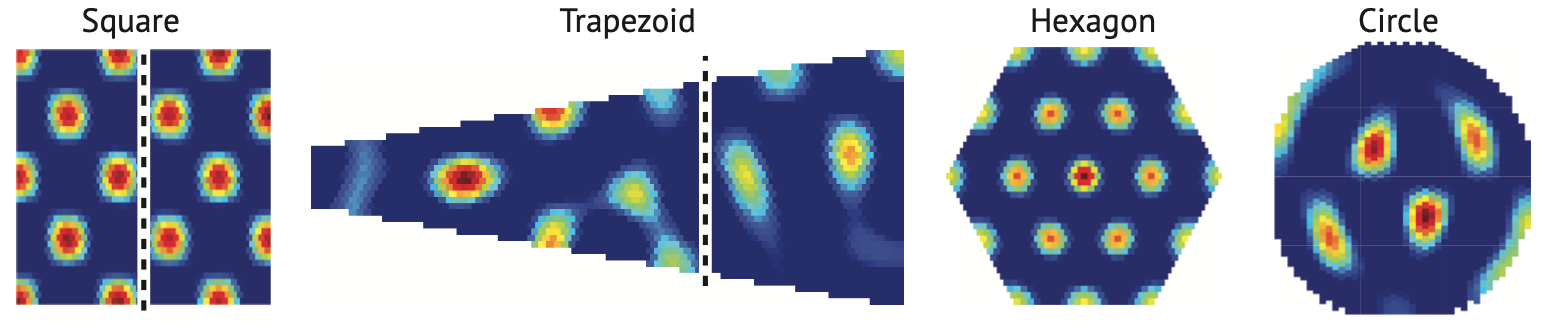
\includegraphics[width=12cm]{successor_repr_sim}
	\caption{Grid cell patterns appearing by simulating agents in environments similar to those from experiments by Krupic et al. (fig. \ref{fig:kurpic}). Each picture shows only one of the eigenvectors. Other eigenvectors would produce different grid patterns.}
	\label{fig:successor_repr_sim}
\end{figure}

\subsubsection{Slow feature analysis}

Another candidate algorithm for explaining emergence of cognitive maps, is the \textit{slow feature analysis} \cite{slow_feature_analysis} (SFA). It is capable of generating grid cells, place cells, head-direction cells, simple and complex cells of V1, and so on \cite{slowness_sparseness}. To the best of my knowledge, it is the only algorithm capable of generating such a wide range of receptive fields, using nothing more than visual stimulus (agent has no direct knowledge of state $s$). 

\textit{Slowness principle} states that the sensory stimulus should be consistent in time and change continuously. Objects do not appear and disappear suddenly, but rather come into and out of agent's view gradually. Similar stimulus signals, that are received closely in time, are likely to come from the same object. This reasoning can be captured more formally. 

Given an input signal $x(t)=[x_1(t),...,x_I(t)]^T$ evolving in time $t\in[t_0,t_1]$, we attempt to find a  function $g(x)=[g_1(x),...,g_J(x)]^T:\mathbb{R}^I\rightarrow \mathbb{R}^J$, such that the output $y(t)=[y_1(t),...,y_J(t)]$ with $y_j(t)=g_j(x(t))$ changes as slowly as possible. 
Formally, we seek to minimize the squared derivative $\langle \dot{y}_j^2 \rangle$,
where angle brackets denote the integral
\[\langle f \rangle = \frac{1}{t_0-t_1} \int_{t_0}^{t_1} f(t) dt\]
In order to prevent trivial solutions (such as constant or duplicated functions $g_j$), we impose further restrictions
\begin{align*}
 \langle y_j \rangle &= 0\text{ (zero mean)}	\\
 \langle y_j^2 \rangle &= 1 \text{ (unit variance)} \\
\forall_{j'< j} \langle y_{j'} y_j \rangle &= 0 \text{ (decorrelation)} \\ 
\end{align*}
This is a minimization problem of variational calculus, which in general case is difficult to solve. In order to narrow down the search space, assume that $g$ is a linear combination of functions $h_k$ from some finite set.
\[
g_j(x) = \sum_{k=1}^K w_{jk} h_k(x)
\] 
where $w_{jk}$ are elements of some weight matrix $\boldsymbol{W}\in \mathbb{R}^{J \times K}$.
If we introduce an auxiliary variable $z(t)=h(x(t))$, we can restate $y$ in vector form 
\[
y_j(t)=g_j(x(t)) = \boldsymbol{w}_j^T h(x(t)) = \boldsymbol{w}_j^T z(t) 
\]
The minimization objective becomes  
\[
\langle \dot{y}_j^2 \rangle = \boldsymbol{w}_j^T \langle \dot{z} \dot{z}^T \rangle \boldsymbol{w}_j
\]
Assume that the functions $h_k$ have been chosen in such a way that $z(t)$ has zero mean and unit covariance matrix. Then the constraints can be simplified to
\begin{align*}
	\langle y_j \rangle &= \langle \boldsymbol{w}_j^T z \rangle = \boldsymbol{w}_j^T  \langle  z \rangle =  \boldsymbol{w}_j^T  \cdot 0 =  0 \\
	\langle y_j^2 \rangle &=  \boldsymbol{w}_j^T \langle z z^T \rangle \boldsymbol{w}_j = \boldsymbol{w}_j^T \textbf{I} \boldsymbol{w}_j = \boldsymbol{w}_j^T \boldsymbol{w}_j  = 1 \\
	\forall_{j' < j} \langle y_{j'} y_j \rangle &= \boldsymbol{w}_{j'}^T \langle z z^T \rangle \boldsymbol{w}_j = \boldsymbol{w}_{j'}^T \textbf{I} \boldsymbol{w}_j = \boldsymbol{w}_{j'}^T \boldsymbol{w}_j = 0 \\ 
\end{align*}
This means that the constraints on $y$ will be fulfilled if we can guarantee that $\boldsymbol{W}$ is orthonormal.  For the first $y_1$, the decorrelation constraint is vacuously true, thus the problem reduces to finding the normed  vector $\boldsymbol{w}_j$ that minimizes $\langle y_1 \rangle$. The solution is obtained by finding the smallest eigenvector of covariance matrix $\langle \dot{z} \dot{z}^T \rangle$. This problem is known as minor component analysis (MCA), and the smallest eigenvalues are called minor components. Each $y_j$ can be minimized by finding the corresponding minor component. Eigenvalues can be found by performing eigendecomposition using any of the methods known from linear algebra. 

In practice, is it more efficient to use an iterative approach, such as \textit{candid covariance-free incremental principal component analysis} and incremental MCA. It also allows for continual learning in a dynamically changing environment. Such approach has been termed \textit{incSFA}. Analogically to deep networks, SFA can produce more complex results when arranged in a multi-layer hierarchical architecture with convolutional connectivity patterns (fig. \ref{fig:inc_sfa_hierarchy}).
\begin{figure}[!htbp]
	\centering
	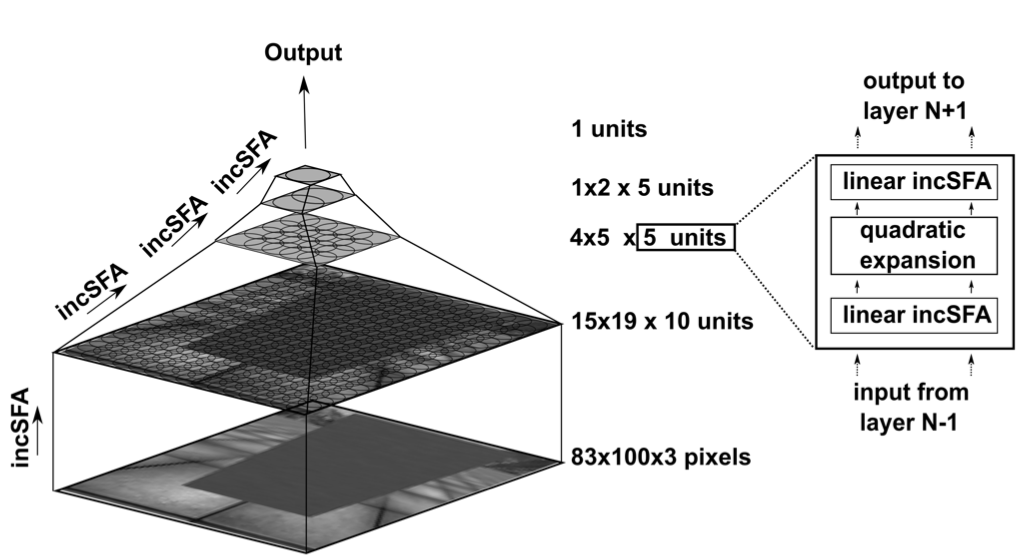
\includegraphics[width=10cm]{inc_sfa_hierarchy}
	\caption{Hierarchical incremental slow-feature-analysis. The connections are localized, analogically to the topology found in convolutional neural networks.}
	\label{fig:inc_sfa_hierarchy}
\end{figure}

It has been found SFA leads to emerge of receptive fields similar to complex cells of primary visual cortex \cite{sfa_complex_cells}. 
By combining slowness principle with sparseness of neural activations, place, grid, head-direction and spacial-view cells can also arise \cite{slowness_sparseness} (fig. \ref{fig:sfa_place_cells}).
\begin{figure}[!htbp]
	\centering
	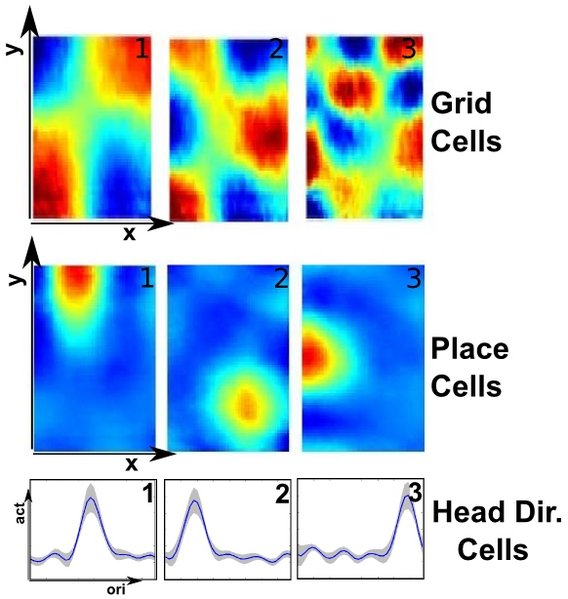
\includegraphics[width=7cm]{ sfa_place_cells}
	\caption{Simulated hippocampal neurons.}
	\label{fig:sfa_place_cells}
\end{figure}

\subsubsection{Tollman-Eichenbaum Machine}

Deep networks trained with backpropagation are capable of producing place cells. To achieve this, a special architecture of \textit{Tollman-Eichenbaum machine} (TEM) \cite{TEM} is required. 

The agent navigates some environment $S$. Each state $s\in S$ produces some signal $x = \xi(s) \in \mathcal{X}$. The agent can only observe $x$ and has no access to $s$. The task is to learn graph structure of $S$. Based on the sequence of actions and observations 
\[
x_1, a_1, x_2, a_2, ... , x_{t-1}, a_{t-1}
\]
agent must predict the next signal $x_{t}$. During training, the agent will experience many trajectories, all of them sharing the same underlying graph $S$, but with a different state-signal mapping $\xi$. This means that some form of episodic memory is required. Predicting $x_{t}$ is only possible if agent knows $S$ and remembers what $\xi(s)$ it has previously seen within the current episode (trajectory). 

TEM solves this learning problem by introducing  $\boldsymbol{g}$, which is an approximation of the unknown $s$. At each time step $t$, we use some fully-connected layers to model $p(\boldsymbol{g}_{t}|\boldsymbol{g}_{t-1},a_t)$, similarly as it is done in recurrent neural networks. Once a new $\boldsymbol{g}_{t}$ is estimated, it is used as a ``query key'' to an attractor-network $M_{t-1}$, which returns a grounded variable $\boldsymbol{p}_{t}$. Attractor networks work by iteratively applying some transformation to their input, until an attractor state (fixed-point) is reached. One example of this are Hopfield networks. In the case of TEM, the attractor network is implemented by a matrix $M$, and the fixed-point is reached by applying
\[
\boldsymbol{h}_{\tau+1} = f_p(\kappa \boldsymbol{h}_{\tau}+\boldsymbol{M}_t \boldsymbol{h}_{\tau})
\]
to some initial input $\boldsymbol{h}_0$ (in this case, $\boldsymbol{h}_0=\boldsymbol{g}_{t}$, and in the limit $\boldsymbol{h}_{\infty}=\boldsymbol{p}_{t}$ is reached) where $f_p$ is some activation function and $\kappa$ is some constant. Having obtained $\boldsymbol{p}_{t}$,  feed-forward layers can be used to model $p(x_{t}| \boldsymbol{p}_{t})$. Thus, the agent can ``imagine'' the next signal. All of the above mechanisms allow us to implement the generative model
\[
p(x_{\le T},\boldsymbol{p}_{\le T}, \boldsymbol{g}_{\le T}) = \prod_{t=1}^T p(x_{t}|\boldsymbol{p}_{t}) p(\boldsymbol{p}_{t}|\boldsymbol{M}_{t-1},\boldsymbol{g}_{t})p(\boldsymbol{g}_{t}|\boldsymbol{g}_{t-1},a_t)
\]

In order to train the network with backpropagation, a loss function and error is necessary. This can be obtained by coupling the generative model with a discriminative one, which has access to signal $x_{t}$ and uses it to build object representation $\boldsymbol{p}_{t}$ and guess location $\boldsymbol{g}_{t}$. Then we can compare $\boldsymbol{p}_{t}$ produced by both models and use a loss function that penalizes squared distance between the two vector representations. The same can be done for $\boldsymbol{g}_{t}$. Discriminative model is implemented as
\[
p(\boldsymbol{g}_{\le T},\boldsymbol{p}_{\le T}|x_{\le T}) = \prod_{t=1}^T
p(\boldsymbol{p}_t|x_{\le t}, \boldsymbol{g}_{t})
p(\boldsymbol{g}_t|x_{\le t},\boldsymbol{M}_{t-1},\boldsymbol{g}_{t-1},a_t) 
\]
The input signal is first preprocessed by appropriate layers and the resulting vector $x_{t}$ is passed as ``query'' into the attractor network $\boldsymbol{M}_{t}$, retrieving some memory $\boldsymbol{p}^{x}_{t}$. Further, recurrent layers are used to model
$p(\boldsymbol{g}_t|\boldsymbol{p}^{x}_{t},\boldsymbol{g}_{t-1},a_t)$ and $p(\boldsymbol{p}_t|\boldsymbol{g}_t,x_t)$. Lastly, the newly produced grounded variable $\boldsymbol{p}_t$ is used to update memory $\boldsymbol{M}_{t-1}$ with the hebbian learning rule
\[
\boldsymbol{M}_{t} = \lambda \boldsymbol{M}_{t-1} + \eta (\boldsymbol{p}_t - \hat{\boldsymbol{p}_t})(\boldsymbol{p}_t + \hat{\boldsymbol{p}_t})^T
\]
where $\lambda$, $\eta$ are some constants and $\hat{\boldsymbol{p}}$ is some vector representing current place (could be $\boldsymbol{p}^{x}_{t}$ or the other $\boldsymbol{p}_t$ produced by generative model). The final schematic of TEM is presented on figure \ref{fig:tolman_eich}.
\begin{figure}[!htbp]
	\centering
	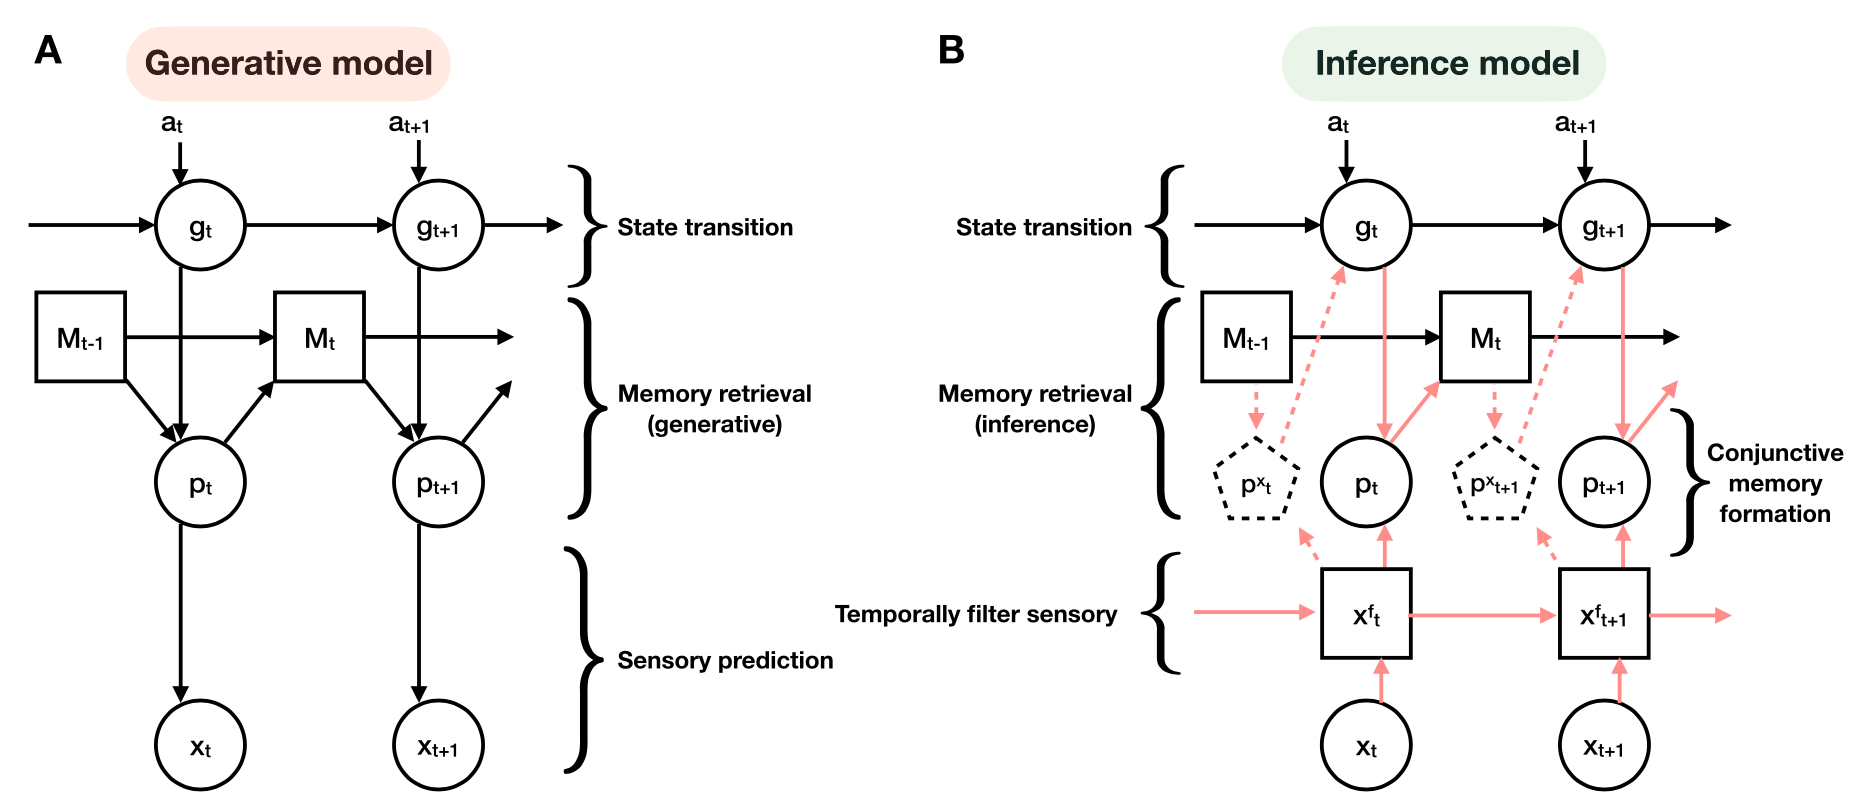
\includegraphics[width=12cm]{tolman_eich}
	\caption{An example of a simple grid-like environment $S$ with different objects (signals $x$) placed in specific locations (states $s$).}
	\label{fig:tolman_eich}
\end{figure} 

The associative memory network $\boldsymbol{M}$ is not trained with backpropagation. It is updated using only hebbian learning rules. Nonetheless, backpropagation-through-time can be applied to the model as a whole, because  retrieving memories from $\boldsymbol{M}$ is a differentiable operation and the matrix $\boldsymbol{M}$ can be treated as a constant. Changes made to $\boldsymbol{M}$ are something that backpropagation can learn to use to its advantage. 

Such use of hebbian learning makes TEM a unique architecture, which may seem to go beyond the scope of geometric deep learning theory. A recent result \cite{TEM_as_teransformer} shows that upon closer examination, Hopfield network $M$ is mathematically equivalent to self-attention and that TEM could be regarded as a transformer. 

Tolman-Eichenbaum machine is a general architecture that can be applied to learn any graph $S$. In the special case of $S$ being a grid (discretized 2-dimensional plane) the activation patterns of $\boldsymbol{g}$ start to resemble grid cells, whereas $\boldsymbol{p}$ functions like place cells (fig \ref{fig:tolman_eich_results}).
\begin{figure}[!htbp]
	\centering
	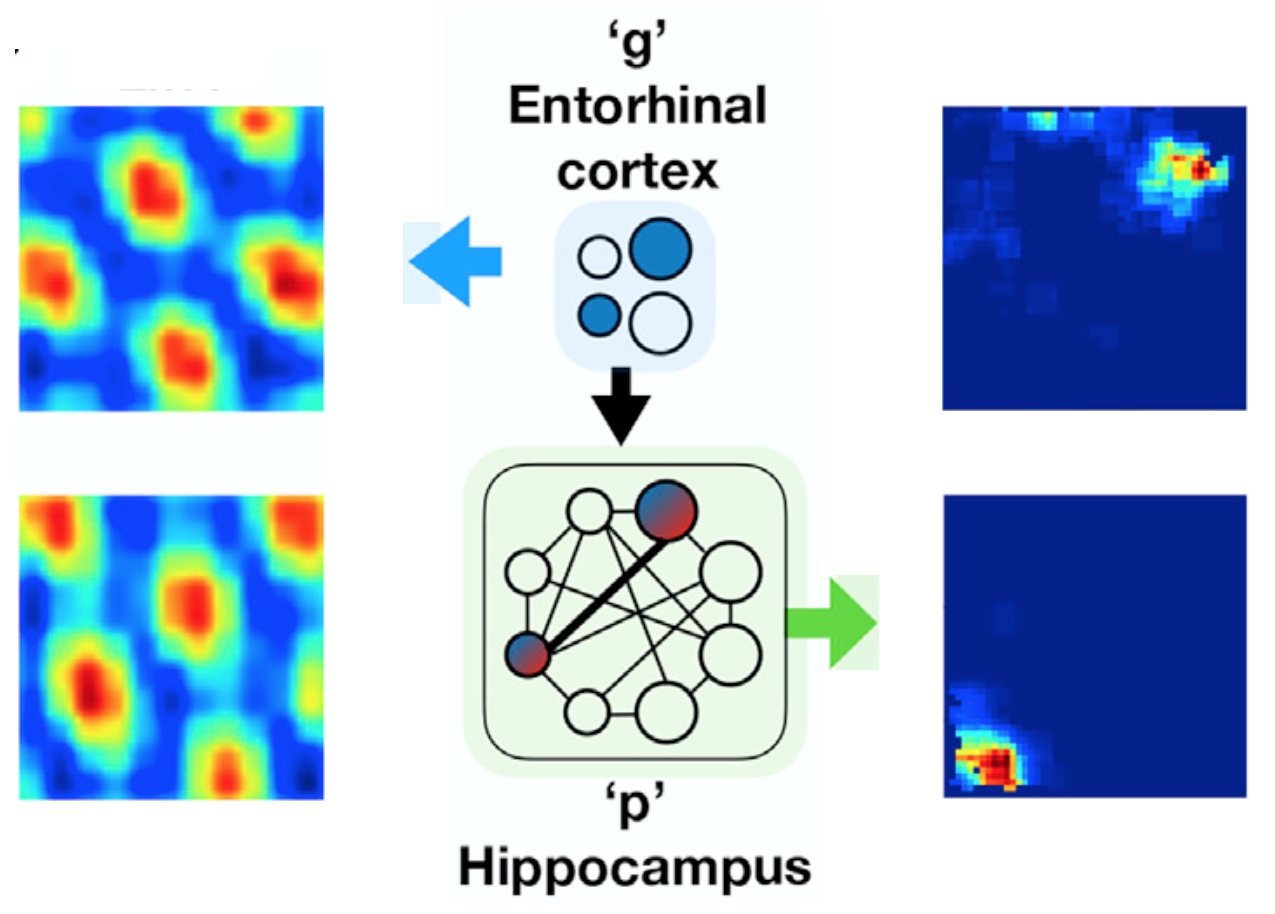
\includegraphics[width=7cm]{tolman_eich_results}
	\caption{Place cells and grid cells emerging in $\boldsymbol{p}$ and $\boldsymbol{g}$ layers of TEM.}
	\label{fig:tolman_eich_results}
\end{figure} 

\section{Geometry of reinforcement learning}

The main results of this thesis are heavily reliant on all the preliminaries introduced in previous sections. Geometric deep learning provided us with a rigorous framework for explaining the success behind deep neural networks. Nearly all modalities such as computer vision, speech recognition, natural language processing, etc. could be (for the most part) considered as ``solved''. Geometric priors gave us a tool for addressing the curse of dimensionality.
The notable outlier is the deep reinforcement learning, which has had a limited applicability in real-world scenarios. I would like to make the argument that sample inefficiency has many similarities to the curse of dimensionality. Algebraic symmetries may likely once again prove to be the key. While I cannot yet provide a functioning solution to the problem, I wish to share my insights, supported by mathematical arguments and ``proof of concept'' experiments. 

\subsection{Sample inefficiency and symmetries}

Let us consider some group $S$. This group acts on a signal space $\mathcal{X}$. Suppose that $S$ is generated by some set $A \subset S$, meaning that every element $s\in S$ can be represented as composition 
\[
s = A_1 A_2 A_3 ... A_t
\]
of one or more elements $A_1,A_2,A_3,...A_t$ of $A$. For example, any whole number $\mathbb{Z}$ can be represented as sum of ones and minus ones, thus $\{-1,1\}$ generates group $\mathbb{Z}$ under operation of addition. 

The classical definition of MDP assumes that the agent always knows the exact state $S_t \in S$. In a real world scenario, an animal or a robot could only see a small fragment of the world through their eyes or other sensors. Thus, we assume that $S_t$ is an unknown latent variable that is accessible to the agent only through some sensory signal $\mathcal{X}$. This is commonly referred to as a \textit{partially observable} MDP. 

The agent can take an action $A_t\in A$, which transitions the current state of the world $S_t$ to a new $S_{t+1}$
\[
S_{t+1} = S_{t}A_t = A_0 A_1 A_2 ... A_t
\]
The group $S$ also acts on the input stimulus $\mathcal{X}$, changing it accordingly. For example, if $x\in\mathcal{X}$ is an image seen from a certain point of view $S_t$, then by moving the agent's head to the left, $x$ will be translated to the right.  Such framework forms a bridge between geometric deep learning theory and reinforcement learning.

The decision tree of an MDP represents all possible trajectories. Formally, it is a graph with set of vertices $A^+$ and edges labelled with actions $A$. Every possible action sequence $A_0A_1A_2...A_t$ is treated like a string $A^+$ over alphabet $A=\{a_1,a_2,...a_n\}$. A set of strings together with operation of concatenation forms a semigroup. Two strings $A_0A_1A_2...A_t$ and $A_0'A_1'A_2'...A_{t'}'$ are equal if and only if they are of the same length $t=t'$ and their corresponding symbols are equal $A_i=A_i'$ for all $0\le i \le t$. Every action $A$ is also a member of the group $S$, therefore every action sequence denotes some element of $S$. It is important to recognize the difference between notation and denotation. For example, $1+1+1$ and $1+2$ are two different notations that both denote the number $3$. Similarly, two different action sequences (moving up and left or left and up) might result in the agent reaching the same final state. 
We say that a semigroup is \textit{free} if no two different notations have the same denotation. In a decision tree, every vertex is considered to be different, because it is treated as a string $A^+$, rather than a state $S$, therefore a decision tree is a free semigroup. If we assume that every action has its inverse (such as moving left and right or rotating clockwise and counter-clockwise), then the decision tree becomes a Cayley graph of a free group.


When trying to learn a value function $v:S\rightarrow \mathbb{R}$, we are faced with an approximation problem. The input to this function is not a signal and does not have a clear definition of dimensionality, but it has some algebraic structure.  The Bellman equation expresses the relationship between neighbouring states $s$ and $sa$ in the Cayley graph.
\[
v_\pi(s) = \sum_{a\in A} \pi(a|s)\big(R(sa)+\gamma v_\pi(sa)\big)
\]
When $S$ is a free semigroup, then the Bellman equation is the only constraint on $v$.
Groups with additional symmetries, will have more constraints. In order to find them, we need to know the \textit{presentation of a group} (or semigroup), defined as
\[
S = \langle A \vert \mathcal{R} \rangle
\]
where $A$ is the generator of $S$ and $\mathcal{R}$ is a set of relations. Each relation has the form of equality between two strings $A^+$ (notations) over $A$
\[
A_0A_1A_2...A_t = A_0'A_1'A_2'...A_{t'}'
\]
For example, a cyclic  group of order $n$ has the presentation $\langle a_0 \vert a_0^n=a_0 \rangle$. If some relation $g=h$ belongs to $\mathcal{R}$ (where $g,h\in A^+$), then any $s\in S$ can be added on both sides $sh=sg$ and the equality must be preserved.  Therefore, knowing the presentation of $S$, we can introduce additional constraints on $v$.  
\[
v(sg) = v(sh) \text{ for all }s\in S 
\]
For example, an agent moving in 2 dimensions, can rotate itself $360^\circ$ and end up in the same state. Therefore, $\mathcal{R}$ could include equality $360^\circ=0^\circ$, resulting in constraint
\[
v(s) = v(s+0^\circ) = v(s+360^\circ) \text{ for all }s\in S
\]
If we could include all geometric priors $\mathcal{R}$ directly in the structure of $v$, then the search space would become much narrower, and reinforcement learning might progress more efficiently. The current approaches naively treat the decision tree as if it was a free group, but in reality it is not. What type of deep architecture are we missing, that could address this problem? Most likely no such architecture exists, for the simple reason that symmetries in the action space are dynamic, can change with the environment and are usually not (fully) known a'priori. This stands in stark contrast with symmetries in the signal space, which can be given a'priori and do not need to change over time.

\subsection{Reducing reward maximization to a graph search}

Let us generalize Markov decision processes to a continuous-time environment. The set of states $S$ is a Lie group and the time step $t$ is a real number. We can introduce the \textit{energy function} $E$
\[
R(t) = \frac{dE(t)}{dt}
\]
Reward is received when the agent finds some source of energy (food) that increases $E$. When $E$ decreases (through movement and other actions) the agent will receive negative reward. 

The integral of $R$ is equivalent to the sum of future rewards $R$, which is the definition of return $G$. This is equal to the energy at some future time $E(T)$
\[
\int_{t=t_0}^{T} R(t) dt = G(T) - G(t_0) = E(T)
\]
Maximization of $G$ is equivalent to searching for sources of energy $E$. If we assume that the reward is plentiful in the environment, then we would need to plan an optimal route that passes through as much $R$ as possible. In such scenario, formulating the problem as energy source search does not provide us with any new insights that reward maximization couldn't give us already. 

The true difference between the two approaches becomes more evident when we assume that the reward is sparse. If there are very few sources of energy in the environment, then finding at least one of them, already has a high probability of maximizing the total return. In such scenario, we might forget about reward maximization and route optimization altogether, and only focus on the search. 

Energy function gives us a way of elegantly solving the exploration and exploitation dilemma. The energy is intrinsic and known to the agent. Therefore, we can introduce a ``hunger'' threshold $h$. The agent shall exploit the environment when $E(t) < h$. If the energy is abundant $E(t)>h$ some of it can be ``wasted'' for exploration. 

This leads us to an alternative formulation of the reinforcement learning problem.
The task of an agent is to learn structure of $S$ during the exploration (or latent learning) phase. Then the exploitation (or reward maximization) phase is formally defined as the search for any source of energy $R$ that is greater than some threshold. If $S$ is discrete, then search can be performed on the learned Cayley graph of $S$. In continuous case we can resort to \textit{rough Cayley graphs} (Analogues of Cayley graphs for topological groups). 

It should be noted that temporal-difference learning of $v$ does not work well with sparse rewards, whereas graph-based search only makes sense under sufficient sparsity. Otherwise, if the reward was easy to find, then the search would always end quickly and find very short myopic paths.

Temporal difference is inefficient. It requires multiple passes over the same state (fig. \ref{fig:dynamic_programming}). Building a graph of $S$ could be much faster, as it requires visiting each state transition only once. If, for example, we impose the geometric prior of $S$ being a 2D grid (as it is the case on fig. \ref{fig:dynamic_programming}), then it becomes enough to only visit every state once and all the missing state transitions can be inferred automatically. Once we know the structure of $S$, then we can use any of the graph-traversal algorithms, such as depth- or breadth-first search. Finding a path to the nearest (sparse) reward will with high probability give results equivalent to following $v$.
\begin{figure}[!htbp]
	\centering
	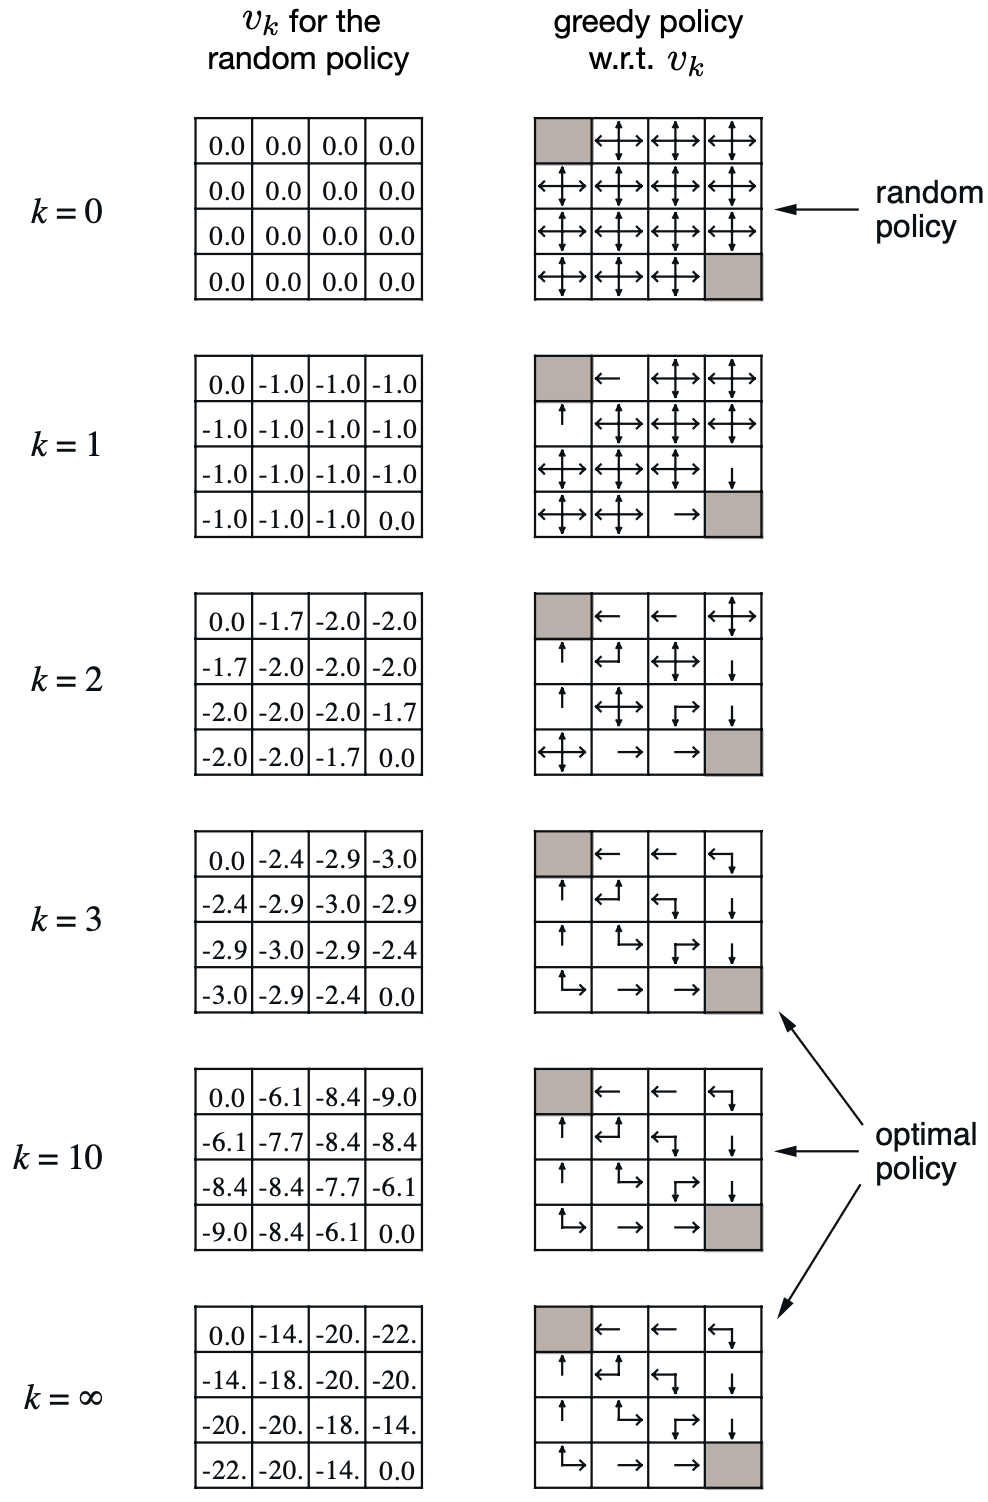
\includegraphics[width=11cm]{dynamic_programming}
	\caption{Policy iteration method can approximate optimal $\pi_*$ and $v_*$ after enough iterations of temporal-difference algorithm. Grey states contain reward. Agent can move up, down, left or right. Policy is indicated by arrows. If there are multiple arrows, then one is chosen at random. $k$ is the iteration number.}
	\label{fig:dynamic_programming}
\end{figure}

\subsection{Representing and navigating Cayley graphs}

The environment $S$ might be large and complex, or even infinite. It might be  impossible to store all of it in computer (or brain) memory. In order to learn it, an efficient representation is necessary. 

The biological brain is good at building cognitive maps, which encode many geometric properties of the world. Grid cells fire in patterns that we could interpret as cosets of 2-dimensional translation group. Place cells represent cosets of even finer granularity. Head-direction cells are cosets of rotation group. Simple cells in primary visual cortex respond to light spots, which resembles cosets of 2-dimensional translation group in retinotopic coordinate system. 

We can take inspiration from nature and model $S$ as several quotient groups $Z$ at different granularity scales. 
\[
S = Z_1 \times Z_2 \times Z_3 \times ... \times Z_k
\]
If each quotient group $Z$ has size $\vert Z \vert$, then the total representational capacity of the cross product is exponential $\vert S\vert = \vert Z_1 \vert  \cdot \vert Z_2 \vert  \cdot ... \cdot \vert Z_k\vert$. 
 
How exactly could such decomposition of $S$ be achieved? It is difficult to decisively tell, which learning algorithm is the ``right'' one. Could it be slow feature analysis, deep neural networks with gradient descent, eigenvalue decomposition of successor representation matrix or something different?  At the moment, we still don't know, but perhaps we could shed some light by asking another question. What data structure do we want to learn? There are several necessary and desirable properties that the ideal data structure should have.

Most environments (especially the natural one) do not allow the agent to replay any event. One-shot learning is necessary, because a second shot might never come.  Moreover the memories should not interfere with each other. Otherwise, learning a new fact about $S$ can cause older memories to be overwritten, which is known as \textit{catastrophic forgetting}. In summary, the data structure that we need must allow us to build a reliable, long-lasting \textit{episodic memory} - something which current deep RL agents do not have. Could deep networks and backpropagation achieve it? 

A Cayley graph could be expressed in differentiable form as a deep network, which takes as input current state $s\in S$ and action $a\in A$, and returns the new state $sa\in S$.  Both $s$ and $a$ would need to be embedded in some real-valued vector spaces. This could pose a problem during graph search, as small error will likely accumulate with each edge traversal. Another problem would be one-shot learning. Suppose the agent observes a new transition $sa=s'$. How many backpropagation steps would be necessary to ensure that the network learns it with satisfactory accuracy (the embedding of $s'$ shouldn't be too distant from $sa$)? Last and perhaps the most serious problem is catastrophic forgetting. We can run backpropagation for as many steps as necessary until we reach the desired accuracy of embeddings, but as a side effect, we might misplace all the previously learned state embeddings. Perhaps a massively large and deep network, would have enough representational capacity to offset this problem, but then the graph search would require accordingly larger computational resources to evaluate such network multiple times. This would come at significant latency and power consumption. 



The real brain does not seem to be working in such a way. It requires very little energy and can respond to stimulus within a few milliseconds. Instead of modelling a function $S\times A \rightarrow S$, we could imitate the brain by modelling states of $S$ as individual neurons. Suppose that for every $s\in S$ there exists one corresponding neuron $n_s$ in the network structure. If the agent transitions from $s$ to $s'$, we could strengthen the connection weight $w_{ss'}$ between $n_s$ and $n_{s'}$. This mechanism is local, which means that it will not interfere and overwrite other memories. It would also not require backpropagation. Hebbian learning rules would be enough. If building a relation between two events is only a matter of connecting the corresponding neurons together, then one-shot learning is easy to achieve. During graph search, we could follow the connections between consecutive states, without the need for activating any intermediate neurons. It is possible to make the graph search highly efficient by initiating activation of some neuron $n_{s}$ that corresponds to current state $s$, and then $n_s$ could simultaneously cause firing of several possible $n_{s'}$ neurons corresponding to different future path candidates. We could use a (parallelized) random walk  as a simple search mechanism. If $S$ is decomposed into multiple quotient groups, then planning could simultaneously occur on different granularity scales. If the strength of connections is proportional to the expected reward, then random walk would be skewed towards ``better'' paths. A mechanism similar to sharp-wave ripple could be used to learn such skewed connection strengths, by replaying recent trajectories $s_0,s_1,s_2,...s_t$, reactivating consecutive neurons $n_{s_0},n_{s_1},...,n_{s_t}$ and incrementing their connections $w_{s_0s_1},...,w_{s_{t-1}s_t}$ by some learning rate proportional to reward. Using a mechanism similar to lateral inhibition, the first random walk that finds  large reward could inhibit other walks running in parallel, thus only the first walk would win. The shortest (most optimal) route would have the highest likelihood of being randomly discovered, thus we could maximize return $G$ without temporal-difference and without performing any explicit function optimisation. We could potentially build episodic memory by assuming temporal consistency, that is if $n_{s'}$ fires after $n_{s}$ then $s'$ occurs after $s$, and therefore entire chains of memories could be built. The only problem is that the number of states $S$ might be large, even if we decompose $S$ into a hierarchy of quotient groups. Within such large networks, only a few neurons would have to be active at the same time. Therefore, the ideal data structure would be a large and sparsely active network.  Instead of representing $s$ with a single $n_{s}$, a sparse population of multiple neurons might be more efficient coding scheme.

The mechanism of planning by performing parallel random walks over cognitive maps is very simple. If it was indeed true that hippocampus worked in this way, then another hypothesis would immediately come to mind. Perhaps higher cognitive functions and human-like intelligence could reuse some of the same mechanism, but at a larger scale. 

\section{Sparse binary winner-takes-all networks}

Rate-coded models of neurons (deep nets, slow feature analysis, predictive coding) often have sophisticated mathematical foundations, but they tend to ignore the temporal aspects of individual spikes, relative firing and latency. More biologically realistic neurons (Hodgkin-Huxley, integrate-and-fire, stimulus response model) use differential equations to simulate the exact temporal evolution of membrane potentials, but they often lack the ``bigger picture'' explanation of algorithms and computations performed by the neurons. 

Sparse binary neuronal assemblies are an attempt to balance the realism and mathematical interpretability of neural models. It is also an important research venue, as we currently lack good learning algorithms for networks with sparse and binary activations. Such data structures would be an ideal candidate for modelling Cayley graphs. 

A departure from continuous values and differential equations could potentially contribute to better understanding of more traditional realistic models from neuroscience. I like to illustrate the premise behind such approach by a simple analogy to digital computers. If we tried to reverse-engineer a CPU in the same way as we study biological neurons, we might try measuring the voltage levels in individual circuits and transistors. An experimented might notice that the voltage evolves continuously in time and can be described by systems of differential equations, but what makes the CPU a ``computer'' is not the physics of electric currents, but rather the discrete zeroes and ones that they represent. The true understanding of biological neurons will not be achieved until we can discretize and formally prove the algorithms that they implement. 

The algorithm, described in the rest of this thesis, is my attempt at finding such a proof.

\subsection{Bayesian and variational inference}

The foundation of all machine learning algorithms is the problem of estimating parameters $\theta$ for some unknown statistical model $p(x;\theta)$, based on a set of observations $x$ generated by $p(x;\theta)$.  Bayesian inference \cite{var_inf} is a process in which evidence $p(\theta)$ and observations $x$ are used to estimate posterior probability $p(x|\theta)$ where $\theta$ is treated like a random variable.
If we are only interested in finding $\theta$ that maximizes $p(x|\theta)$,  we can use \textit{maximum likelihood} (ML) estimation
\[
\hat{\theta}_{ML} = \argmax_\theta p(x;\theta)
\]
In many cases, the likelihood function $p(x;\theta)$ might be expensive to evaluate and using exhaustive search over the entire parameter space is not feasible. This problem can be alleviated by introducing a hidden variable $y$ and then reformulating $p(x;\theta)$ as marginal distribution 
\[
p(x;\theta) = \int p(x, y;\theta) dy = \int p(x|y;\theta) p(y;\theta)  dy
\]
Using Bayes' theorem, we can also obtain posterior distribution of hidden variables
\[
p(y|x;\theta) = \frac{p(x|y;\theta)p(y;\theta)}{p(x;\theta)}
\]
The main difficulty in applying Bayesian inference is that the integral over $y$ is often impossible to compute directly. A different technique called \textit{maximum posteriori} (MAP) inference allows us to avoid integration as follows
\[
\hat{\theta}_{MAP} = \argmax_\theta p(\theta|x) = \argmax_\theta \frac{p(x|\theta)p(\theta)}{\int p(x|\theta)p(\theta) d\theta} = \argmax_\theta p(x|\theta)p(\theta)
\]
because the denominator becomes a constant and no longer depends on $\theta$.
MAP can be combined with \textit{expectation maximization} (EM) \cite{em_alg} algorithm by taking logarithm and introducing some distribution function $q(y)$
\[
\ln p(\theta | x) = F(q,\theta) + KL(q\Vert p) 
\]
where $F$ is the free-energy
\[
F(q,\theta) = \int q(y) \ln \frac{p(x,y;\theta)}{q(y)} dy
\]
and $KL$ is the Kullback-Leibler divergence
\[
KL(q\Vert p) = -\int  q(y)\ln(\frac{p(y|x;\theta)}{q(y)}) dy
\]
It always holds that $KL(q\Vert p) > 0$, therefore $\ln p(\theta | x) > F(q,\theta)$,  meaning that free-energy is the lower bound of  log-likelihood. 
In the E-step of EM algorithm, this lower  bound is maximized with respect to $q(y)$. In the M-step $q$ is held fixed and $F$ is maximized with respect to $\theta$.
When repeated, such procedure causes $q(y)$ to converge to $p(y|x;\theta)$. 
This forms the basis of variational inference \cite{var_inf}. It is the foundation for predictive coding \cite{pred_coding, free_energy_principle_and_brain}, which has been shown to approximate backpropagation using biologically-plausible hebbian learning rules \cite{pred_coding_comp_graph}. Large networks of neurons can be modelled by using multiple hidden variables  $\boldsymbol{y}=[y_1,...,y_m]$
\[
\boldsymbol{q}(\boldsymbol{y}) = \prod_{j=1}^{m} q(y_j)
\]
The above product holds true under the assumption that all variables are independent. \textit{Graphical models} can be used to further introduce conditional dependencies. 

\subsection{Partitioning $p$ into mutually exclusive classes}

I  propose an algorithm called \textit{exclusive coincidence classes} (ECC), which takes a shortcut and models the marginal distribution directly.
Instead of assuming that $y_j$ are mutually independent, let us assume that they are mutually exclusive, meaning that only one of them can be true at the same time. This imposes the restriction that all $y_j$ must be boolean random variables $y_j\in\{0,1\}$, and $\boldsymbol{y} \in \mathcal{Y} = \{0,1\}^m$ is a one-hot binary vector. To stay consistent, let the observations $\boldsymbol{x}\in \mathcal{X} = \{0,1\}^n$ be a binary vector as well, but not necessarily one-hot. A key assumption is that to every observation $\boldsymbol{x}$ corresponds exactly one explanation $y_j$ (formally the space $\mathcal{X}$ is partitioned into $m$ classes), therefore we write $p(\boldsymbol{x}|y_j)$ as a short notation for $p(\boldsymbol{x}|\boldsymbol{y})$ where $y_j$ is true.

Observations  $\boldsymbol{x}$ come from an unknown probability distribution $p(\boldsymbol{x})$. The task is to find model $q(\boldsymbol{x})$ that matches $p(\boldsymbol{x})$ as closely as possible. This is achieved by assuming that every observation is conditional only on its explanation $q(\boldsymbol{x}|y_j)$
\[
q(\boldsymbol{x}) = \sum_{j=1}^m q(\boldsymbol{x}|y_j)p(y_j)
\]
We are not interested in modelling $q(y_j)$. It should not matter how often any explanation occurs, thus allowing for some degree of out-of-distribution learning. 
It is assumed that bits $x_i$ generated by the same explanation $y_j$ are mutually independent 
\[
q(\boldsymbol{x}|y_j) = \prod_{i=1}^n q(x_i|y_j)
\]
Distribution $q(\boldsymbol{x}|y_j)$ specifies, which $x_i$ often co-occur together when $y_j$ is activated. We could say that $y_j$ variables are ``coincidence detectors''.  
\begin{figure}[!htbp]
	\centering
	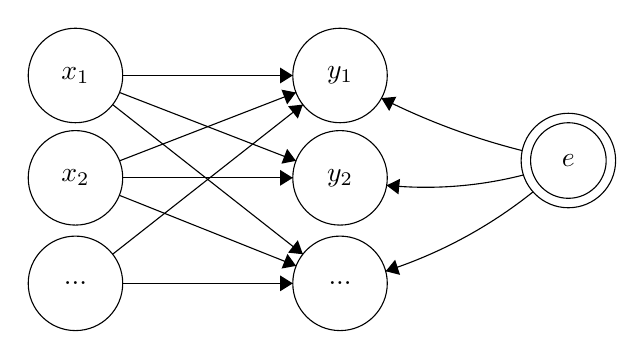
\begin{tikzpicture}[scale=0.2]
		\tikzstyle{every node}+=[inner sep=0pt]
		\draw [black] (40.1,-42.4) circle (3);
		\draw (40.1,-42.4) node {$e$};
		\draw [black] (40.1,-42.4) circle (2.4);
		\draw [black] (25.6,-37) circle (3);
		\draw (25.6,-37) node {$y_1$};
		\draw [black] (25.6,-43.5) circle (3);
		\draw (25.6,-43.5) node {$y_2$};
		\draw [black] (25.6,-50.2) circle (3);
		\draw (25.6,-50.2) node {$...$};
		\draw [black] (8.8,-37) circle (3);
		\draw (8.8,-37) node {$x_1$};
		\draw [black] (8.8,-43.5) circle (3);
		\draw (8.8,-43.5) node {$x_2$};
		\draw [black] (8.8,-50.2) circle (3);
		\draw (8.8,-50.2) node {$...$};
		\draw [black] (37.168,-41.77) arc (-104.11092:-116.74113:43.351);
		\fill [black] (28.23,-38.44) -- (28.72,-39.25) -- (29.17,-38.35);
		\draw [black] (37.246,-43.318) arc (-75.60821:-95.71526:24.95);
		\fill [black] (28.56,-43.98) -- (29.31,-44.55) -- (29.41,-43.56);
		\draw [black] (37.857,-44.391) arc (-51.32615:-72.11948:29.448);
		\fill [black] (28.5,-49.43) -- (29.41,-49.66) -- (29.1,-48.7);
		\draw [black] (11.8,-37) -- (22.6,-37);
		\fill [black] (22.6,-37) -- (21.8,-36.5) -- (21.8,-37.5);
		\draw [black] (11.6,-42.42) -- (22.8,-38.08);
		\fill [black] (22.8,-38.08) -- (21.88,-37.9) -- (22.24,-38.84);
		\draw [black] (11.16,-48.35) -- (23.24,-38.85);
		\fill [black] (23.24,-38.85) -- (22.3,-38.95) -- (22.92,-39.74);
		\draw [black] (11.6,-38.08) -- (22.8,-42.42);
		\fill [black] (22.8,-42.42) -- (22.24,-41.66) -- (21.88,-42.6);
		\draw [black] (11.16,-38.85) -- (23.24,-48.35);
		\fill [black] (23.24,-48.35) -- (22.92,-47.46) -- (22.3,-48.25);
		\draw [black] (11.8,-43.5) -- (22.6,-43.5);
		\fill [black] (22.6,-43.5) -- (21.8,-43) -- (21.8,-44);
		\draw [black] (11.8,-50.2) -- (22.6,-50.2);
		\fill [black] (22.6,-50.2) -- (21.8,-49.7) -- (21.8,-50.7);
		\draw [black] (11.59,-44.61) -- (22.81,-49.09);
		\fill [black] (22.81,-49.09) -- (22.26,-48.33) -- (21.89,-49.26);
	\end{tikzpicture}
	\caption{An example of graphical model for ECC network. Node with double outline is ``inhibitory''. All $y$'s connected to it are mutually exclusive. Arrows coming from $x_i$ to $y_j$ correspond to conditional distributions $p(x_i|y_j)$.}
	\label{fig:ecc_graphical_models}
\end{figure}
It is possible to represent $q$ as a ``graphical model'', by introducing a special type of ``inhibitory'' nodes. All variables connected to the same ``inhibitory'' node are mutually exclusive. Figure \ref{fig:ecc_graphical_models} shows the simplest example of such a model. More complex networks will be presented later.

In order to gain some intuition, let us consider the following example. Image observing a straight metal bar. As it rotates in front of your eyes, it will cast a line-shaped shadow on your retina $\boldsymbol{x}$. We might choose to treat different  rotations as distinct ``events'' and use $y_1...y_4$ to denote the angles $0^{\circ},45^{\circ},90^{\circ},135^{\circ}$ respectively. The bar cannot exist in two positions simultaneously, motivating our earlier assumption of mutual exclusivity. This stands in contrast to rate-coded models, which would instead try to assign some fractional probabilities to different explanations $y$, should the bar find itself in some intermediate position (like $20^\circ$ angle). A similar scenario is observed when looking at Rubin's vase illusion. A rate-coded model might assign 50\% probability to vase and 50\% to face classes, but ECC (and human perception) can only see one.

\subsection{Formal proof of convergence}
Now that ECC networks have been introduced, a more rigorous treatment is due.
First, we start by introducing sparse binary vectors.

\paragraph{Binary vector subsets and their overlap probabilities} 

We define cardinality $\lVert\boldsymbol{x}\rVert_1$ as the number of $1$ bits in a given binary vector $\boldsymbol{x}$.

The number of all binary vectors $\boldsymbol{x}$ of length $n$ and cardinality $\lVert\boldsymbol{x}\rVert_1=b$ is
\[\binom{n}{b}\]
The $\ell_1$ norm induces a metric $\lVert\boldsymbol{x}-\boldsymbol{x}'\rVert_1$ on  binary vectors that measures how many bits differ in $\boldsymbol{x}$ and $\boldsymbol{x}'$. The inner product $\langle\boldsymbol{x},\boldsymbol{x}'\rangle$ measures the number of overlapping $1$ bits. 
Given a specific $\boldsymbol{x}$, the number of all possible vectors $\boldsymbol{x}'$ that overlap with it in exactly $b$ bits is 
\[
\Omega(b)=|\{x':\langle\boldsymbol{x},\boldsymbol{x}'\rangle=b\}|=\binom{\lVert\boldsymbol{x}\rVert_1}{b}\binom{n-\lVert\boldsymbol{x}\rVert_1}{\lVert\boldsymbol{x}'\rVert_1-b}
\]
Therefore, the probability that randomly chosen $\boldsymbol{x}'$ overlaps with $\boldsymbol{x}$ in at least $b$ bits is
\[p(\langle\boldsymbol{x},\boldsymbol{x}'\rangle\ge b )=\frac{\sum_{\dot{b}=b}^{\lVert\boldsymbol{x}'\rVert_1}\Omega(\dot{b})}{\binom{n}{\lVert\boldsymbol{x}\rVert_1}}\]
The probability of random $\boldsymbol{x}'$ being a subset of $\boldsymbol{x}$ is
\[p(\boldsymbol{x}'\subset\boldsymbol{x})=\frac{2^{\lVert\boldsymbol{x}\rVert_1}}{\binom{n}{\lVert\boldsymbol{x}\rVert_1}}\]
Both of those probabilities decrease factorially quickly with length $n$. For very sparse vectors, the chance of accidental overlap is almost zero. 

\paragraph{Formal definition of (first-order) ECC network}
Let us formally define ECC as a tuple $(Q,D_W,u,C,\boldsymbol{a})$. Matrix $Q\in \mathbb{R}^{n\times m}$ stores values of $q(x_i|y_j)$. Set $D_W$ specifies the domain of scalar values for some weight matrix $W\in D_W^{n \times m}$. Constant $u$ defines some norm $\ell_u$.  Vector $\boldsymbol{a}$ imposes length constraint on $\lVert W_j \rVert_u=a_j$ where $W_j\in D_W^n$ is the $j^{th}$ column of $W$. Set $C$ defines some partitioning (clustering) of input space $\boldsymbol{x}\in \{0,1\}^n$ into $m$ non-overlapping subsets $C(y_j) $.
Weights $W$ are defined as
\begin{gather*}
	W_j = \argmax_{W_j\in D_W^{n}} \mathbb{E}_p(\boldsymbol{x}W_j|y_j)\text{ where } \lVert W_j \rVert_u=a_j \\
	\mathbb{E}_p(\boldsymbol{x}W_j|y_j) = \sum_{\boldsymbol{x}\in C(y_j)}\boldsymbol{x}W_jp(\boldsymbol{x}|y_j) \\ 
	p(\boldsymbol{x}|y_j) = \frac{p(\boldsymbol{x},y_j)}{p(y_j)} \\
	p(y_j) =  \sum_{\boldsymbol{x}\in \{0,1\}^n}p(\boldsymbol{x},y_j)
\end{gather*}
The clustering assigns every $\boldsymbol{x}$ to its respective $C(y_j)$. Therefore 
\[
p(\boldsymbol{x},y_j) = \begin{cases}
	p(\boldsymbol{x}) & \boldsymbol{x} \in C(y_j) \\
	0 & \boldsymbol{x} \notin C(y_j)
\end{cases}
\]
As a result, we can simplify $p(\boldsymbol{x}|y_j)$ and $p(y_j)$ to
\begin{gather*}
p(\boldsymbol{x}|y_j) = \frac{p(\boldsymbol{x})}{p(y_j)}, \text{ where  }\boldsymbol{x} \in C(y_j)\\
p(y_j) =  \sum_{\boldsymbol{x}\in C(y_j)}p(\boldsymbol{x})
\end{gather*}
The distribution $p(\boldsymbol{x}|y_j)$ is not known and the exact $W_j$ cannot be computed. Instead, ECC network attempts to approximate $p$ using $q$ 
\[
p(\boldsymbol{x}|y_j) \approx q(\boldsymbol{x}|y_j)
\]
First-order ECC networks model the distribution $q$ using the matrix $Q$. 
In the case of $\ell_1$ and $\ell_2$, it is possible to compute $W_j$ using only  $Q$ and without having to model $q(\boldsymbol{x}|y_j)$ directly.

\paragraph{Learning is achieved by maximizing $q(\boldsymbol{x}|y_k)$}
The probability $q(\boldsymbol{x})$ is modelled as
\[
q(\boldsymbol{x}) = \sum_{j=1}^{m} q(\boldsymbol{x}|y_j)p(y_j)
\]
We can find good approximation $q(\boldsymbol{x})\approx p(\boldsymbol{x})$, by ensuring that $q(\boldsymbol{x}|y_j)\approx p(\boldsymbol{x}|y_j)$. 
\begin{gather*}
	q(\boldsymbol{x}) \approx p(\boldsymbol{x}) \\
	\sum_{j=1}^{m} q(\boldsymbol{x}|y_j)p(y_j) \approx \sum_{j=1}^{m} p(\boldsymbol{x}|y_j)p(y_j) \\
	\sum_{j=1}^{m} q(\boldsymbol{x}|y_j)p(y_j)  \approx p(\boldsymbol{x}|y_k)p(y_k) \text{ where }\boldsymbol{x}\in C(y_k)
\end{gather*}
By subtracting $p(\boldsymbol{x}|y_k)p(y_k)$ from both sides, it implies that $ q(\boldsymbol{x}|y_j)$ should be minimized for all $j$ such that $\boldsymbol{x}\notin C(y_j)$
\[
	\sum_{j\ne k} q(\boldsymbol{x}|y_j)p(y_j) \approx 0 
\]
Minimization of $q(\boldsymbol{x}|y_k)$ for $\boldsymbol{x}\notin C(y_k)$ is equivalent to maximization of $\sum_{\boldsymbol{x}\in C(y_k)}q(\boldsymbol{x}|y_k)$ because probabilities sum up to $1$. 
\[
\sum_{\boldsymbol{x}\in\{0,1\}^n} \sum_{j=1}^{m} q(\boldsymbol{x}|y_j)p(y_j) = 1
\]
If $\sum_{\boldsymbol{x}\notin C(y_j)} q(\boldsymbol{x}|y_j)$ decreases across all $y_j$ and $p(y_j)$ stay constant then the following sum decreases
\[
\sum_{j} \sum_{\boldsymbol{x}\notin C(y_j)} q(\boldsymbol{x}|y_j) p(y_j) = \sum_{\boldsymbol{x}} \sum_{j\ne k}  q(\boldsymbol{x}|y_j) p(y_j) \text{ where }\boldsymbol{x}\in C(y_k)
\]
Therefore, it can be seen that maximization of $\sum_{\boldsymbol{x}\in C(y_k)}q(\boldsymbol{x}|y_k)$ will push $q$ closer to $p$. This observation is fortunate, because hebbian learning rules strengthen connections to those $\boldsymbol{x}$ that cause $y_j$ to fire.

\paragraph{Clustering problem measured with overlap}
We can measure quality of cluster $C(y_j)$ as the expected overlap $\langle \boldsymbol{x}, \boldsymbol{x}'\rangle$ (number of $1$ bits in common) of two binary vectors  randomly drawn from the distribution $p(\boldsymbol{x}|y_j)$.
\[
\mathbb{E}_p(\langle \boldsymbol{x}, \boldsymbol{x}'\rangle|y_j) = \sum_{\boldsymbol{x},\boldsymbol{x}'\in C(y_j)} \langle \boldsymbol{x}, \boldsymbol{x}'\rangle p(\boldsymbol{x}|y_j)p(\boldsymbol{x}'|y_j)
\]
The expectation of any two vectors overlapping in a specific bit $x_i$ is given by
\begin{gather*}
p(x_i|y_j) = \sum_{\substack{\boldsymbol{x}\in C(y_j)\\x_i=1}} p(\boldsymbol{x}|y_j)	= \sum_{\boldsymbol{x}\in C(y_j)} x_i p(\boldsymbol{x}|y_j)	= \mathbb{E}(x_i|y_j)\\
\mathbb{E}_p(x_i x_i' | y_j) = \sum_{\boldsymbol{x},\boldsymbol{x}'\in C(y_j)}  x_i x_i' p(\boldsymbol{x}|y_j)p(\boldsymbol{x}'|y_j) = 	\sum_{\substack{\boldsymbol{x},\boldsymbol{x}'\in C(y_j) \\ x_i=x_i'=1}} p(\boldsymbol{x}|y_j)p(\boldsymbol{x}'|y_j) = \\
= \sum_{\substack{\boldsymbol{x}\in C(y_j) \\ x_i=1}} p(\boldsymbol{x}|y_j) \sum_{\substack{\boldsymbol{x}'\in C(y_j) \\ x_i'=1}} p(\boldsymbol{x}'|y_j) = 
\sum_{\substack{\boldsymbol{x}\in C(y_j) \\ x_i=1}} p(\boldsymbol{x}|y_j) \mathbb{E}(x_i'|y_j)= \\
= \mathbb{E}(x_i'|y_j) \sum_{\substack{\boldsymbol{x}\in C(y_j) \\ x_i=1}} p(\boldsymbol{x}|y_j) = \mathbb{E}(x_i'|y_j) \mathbb{E}(x_i|y_j) = \mathbb{E}(x_i|y_j)^2
\end{gather*}
Therefore, the expected value of overlap can be rewritten as  
\begin{gather*}
\mathbb{E}_p(\langle \boldsymbol{x}, \boldsymbol{x}'\rangle|y_j) =  \sum_{\boldsymbol{x},\boldsymbol{x}'\in C(y_j)} \big(\sum_{i=1}^n x_i x_i'\big)  p(\boldsymbol{x}|y_j)p(\boldsymbol{x}'|y_j) = \\
= \sum_{i=1}^n \sum_{\boldsymbol{x},\boldsymbol{x}'\in C(y_j)}  x_i x_i'  p(\boldsymbol{x}|y_j)p(\boldsymbol{x}'|y_j) = \sum_{i=1}^n \mathbb{E}(x_i|y_j)^2 = \lVert \mathbb{E}(\boldsymbol{x}|y_j) \rVert_2^2
\end{gather*}

\paragraph{Expected overlap and $Q$ matrix} 
The expected overlap can be expressed in terms of the matrix $Q$
\[
\mathbb{E}(\langle \boldsymbol{x}, \boldsymbol{x}'\rangle|y_j) = \lVert \mathbb{E}(\boldsymbol{x}|y_j) \rVert_2^2 =  \lVert Q_j \rVert_2^2
\]
or as a dot product $\boldsymbol{x}Q$
\begin{gather*}
	\mathbb{E}_p(x_i x_i' | y_j) = 
	\sum_{\substack{\boldsymbol{x}\in C(y_j) \\ x_i=1}} p(\boldsymbol{x}|y_j) \mathbb{E}(x_i'|y_j)= \mathbb{E}_p\big(x_i \mathbb{E}(x_i'|y_j) \big| y_j\big) = \mathbb{E}_p\big(x_i p(x_i|y_j) \big| y_j'\big)\\
	\mathbb{E}_q(\langle \boldsymbol{x}, \boldsymbol{x}'\rangle|y_j) = \mathbb{E}(\boldsymbol{x} Q_j | y_j)
\end{gather*}

\paragraph{Zero-order ECC networks}
In the first-order ECC network, we defined weights by finding $W_j$ that maximize product $\boldsymbol{x}W_j$
\begin{gather*}
	W_j = \argmax_{W_j\in D_W^{n}} \mathbb{E}_p(\boldsymbol{x}W_j|y_j)\text{ where } \lVert W_j \rVert_u=a_j
\end{gather*}
In zero-order ECC network we assume that $Q=W$. Then maximization of $\boldsymbol{x}W$ is synonymous with maximization of both $\boldsymbol{x}Q$ and $\mathbb{E}(\langle \boldsymbol{x}, \boldsymbol{x}'\rangle|y_j) $. 
The implication holds trivially by equality
\[
\boldsymbol{x}W_j \le \boldsymbol{x}W_h  \implies  \boldsymbol{x}Q_j \le \boldsymbol{x}Q_h 
\]
\paragraph{Optimal clustering maximizes $p(\boldsymbol{x}|y_k)$} 
The effectiveness of neurons depends on their ability to maximize $q(\boldsymbol{x}|y_j)$ for all inputs that belong to a given cluster $\boldsymbol{x}\in C(y_j)$ and minimize $q(\boldsymbol{x}|y_j)$ for those that don't  $\boldsymbol{x}\notin C(y_k)$. In an ideal case $q(\boldsymbol{x}|y_j)$ would be $0$ for all $\boldsymbol{x}\notin C(y_j)$. 

The $Q$ matrix is not capable of fitting every distribution $q(\boldsymbol{x}|y_k)$.
If we assume that
\[
C(y_j) = \{\boldsymbol{x}:j=\argmax \boldsymbol{x}W\}
\]
then the network could use $W$ matrix to optimally cluster $\boldsymbol{x}$ in a way that makes the task of fitting $q(\boldsymbol{x}|y_j)$ easier for $Q$. If we can show
\[
\boldsymbol{x}W_j \le \boldsymbol{x}W_h  \implies  \boldsymbol{x}Q_j \le \boldsymbol{x}Q_h 
\]
then it would imply that maximization of $\boldsymbol{x}W_j$ leads to higher overlap
$\mathbb{E}(\langle \boldsymbol{x}, \boldsymbol{x}'\rangle|y_j) $. If most inputs $\boldsymbol{x}\in C(y_j)$ share many bits in common, then $Q_j$ can better fit $p(\boldsymbol{x}|y_j)$ by assigning higher probabilities only to those highly frequent bits and near-zero everywhere else. This leads to agreement between $p$ and $q$. 



\paragraph{Expected value $\mathbb{E}_{p}(\boldsymbol{x}|y_j)$ maximizes $\boldsymbol{x}W_j$ under $\ell_2$ norm} 

We wish to maximize the expected value of $\boldsymbol{x}W_j$
\[
\mathbb{E}_{p}(\boldsymbol{x}W_j|y_j)=\sum_{\boldsymbol{x}\in C(y_j)} \boldsymbol{x} W_j p(\boldsymbol{x}|y_j)
\]
 under the constraint $\lVert W_j \rVert_2 = a_j$ for some constant $a_j$.  To find the optimal $W_j$, we can use the method of Lagrange multipliers
\[
L(W_j,\lambda) = \sum_{\boldsymbol{x}\in C(y_j)} \boldsymbol{x} W_j p(\boldsymbol{x}|y_j) + \lambda(1- W_j^{T}W_j )
\]
The term $\lambda(1- W_j^{T}W_j)$ will be $0$ only when $W_j$ is a unit vector.
We can take the derivatives 
\begin{gather*}
	\frac{d L}{d w_{ij}} = \sum_{\boldsymbol{x}\in C(y_j)} x_i p(\boldsymbol{x}|y_j) - 2\lambda w_{ij} \\
	\frac{d L}{d \lambda} = 1 - W_j^{T}W_j
\end{gather*}
and solve for $\frac{d L}{d w_{ij}}=0$
\[
W_j = \frac{1}{2\lambda }\sum_{\boldsymbol{x}\in C(y_j)} \boldsymbol{x} p(\boldsymbol{x}|y_j)  = \frac{1}{2\lambda } \mathbb{E}_{p}(\boldsymbol{x}|y_j)
\]
By taking the second derivative we can show that this is indeed a local maximum.
The problem is convex (there is only one extremum), because all observations are binary vectors (Frechet mean on $S^{n-1}$ unit sphere is unique if all points lie on the same hemisphere) and the expected value $\mathbb{E}_{p}(\boldsymbol{x}|y_j)$ will never be a zero vector.

It should be noted that such expected value will be skewed more towards the $\boldsymbol{x}$ with greater cardinality. To avoid any biases, it is necessary to normalize the vectors 
\[
\mathbb{E}_{p}\big(\frac{\boldsymbol{x}}{\lVert \boldsymbol{x} \rVert_2}W_j|y_j \big)= \sum_{\boldsymbol{x}\in C(y_j)} \frac{\boldsymbol{x}}{\lVert \boldsymbol{x} \rVert_2} W_j p(\boldsymbol{x}|y_j)
\]


\paragraph{One-hot vector maximizes $\boldsymbol{x}W$ under $\ell_1$ norm}
We wish to maximize the expected value of $\boldsymbol{x}W_j$ 
\[
\mathbb{E}_{p}(\boldsymbol{x}W_j|y_j)=\sum_{\boldsymbol{x}\in C(y_j)} \boldsymbol{x} W_j p(\boldsymbol{x}|y_j) \text{ where } \lVert W_j \rVert_1=1
\]
sampled according to some distribution $p(\boldsymbol{x}|y_j)$ from a given set $\boldsymbol{x}\in C(y_j)$.  The sum can be rewritten as
\[
\sum_{\boldsymbol{x}\in C(y_j)} \boldsymbol{x} W_j p(\boldsymbol{x}|y_j) = \mathbb{E}_{p}(\boldsymbol{x} W_j|y_j) = \mathbb{E}_{p}(\boldsymbol{x}|y_j)W_j
\]
because $\mathbb{E}$ is a linear operator. The value of $\mathbb{E}_{p}(\boldsymbol{x}|y_j)$ is some real vector $\mathbb{R}^n$.  It can be observed that $\mathbb{E}_{p}(\boldsymbol{x}|y_j)W_j$ is maximized when $W_j$ is a one-hot vector with $w_{ij}=1$ for such $i$ where $p(x_i|y_j)$ is maximal. 

\paragraph{Generalized $a_j$-hot vector maximizes $\boldsymbol{x}W$ under $\ell_1$ norm}
The result above can be generalized for $\lVert W_j \rVert_1 = a_j$ where $a_j$ is any positive constant, not just $1$. When $a_j=1$, then we have a guarantee that $w_{ij}\le 1$ for all $i$. Hence, our original definition of $W_j$ was a real vector $W_j\in \mathbb{R}^n$, but implicitly it was only $W_j\in [0,1]^n$. 

When $a_j\ne 1$, then we must be explicit and state exactly the allowed range of values for $w_{ij}$. Let us consider a scenario where $a_j\in\mathbb{N}^+$ and $W_j\in [0,1]^n$, then the value of $W_j$ that maximizes $\mathbb{E}_{p}(\boldsymbol{x}|y_j)W_j$ is an $a_j$-hot vector with $w_{ij}=1$ for all $i$ such that $p(x_i|y_j)$ is among the top $a_j$ highest probabilities. 

If $a_j\in\mathbb{R}^+$ and $W_j\in [0,1]^n$ then we can maximize $\mathbb{E}_{p}(\boldsymbol{x}|y_j)W_j$ using similar strategy. First, we find the $\lfloor a_j \rfloor$ highest values $p(x_i|y_j)$ and assign $w_{ij}=1$ for all those $i$. Lastly, we find the $\lfloor a_j \rfloor+1$ highest value of $p(x_i|y_j)$ and assign the remaining fractional value to $w_{ij}=a_j - \lfloor a_j \rfloor$. 

For example, let 
$\mathbb{E}_{p}(\boldsymbol{x}|y_j) = [0.2,0.3,0.8,0.7,0.4]$ . If $a_j=3$ then maximal $\mathbb{E}_{p}(\boldsymbol{x}|y_j)W_j$ is obtained for 
$W_j=[0,0,1,1,1]$. If $a_j=2.3$ then maximum is at $W_j=[0,0,1,1,0.3]$.

\paragraph{Proof of k-means convergence for first-order networks}
Start with some arbitrary $C^{(0)}$ at time step $t=0$. Given $C^{(t)}$ compute $Q^{(t)}$
\[
Q^{(t)}_j = \mathbb{E}_p(\boldsymbol{x}|y_j)
\]
Given $C^{(t)}$ and $Q^{(t)}$ compute weights $W^{(t)}$
\begin{gather*}
	W_j^{(t)} = \argmax_{W_j\in D_W^{n}} \mathbb{E}_p(\boldsymbol{x}W_j|y_j)\text{ where } \lVert W_j \rVert_u=a_j
\end{gather*}
Given $W^{(t)}$ compute new clusters $C^{(t)}$
\[
C^{(t+1)}(y_j) = \{\boldsymbol{x} : j=\argmax(\boldsymbol{x}W^{(t)})\}
\]
To show that convergence is guaranteed, let us define a fitness function
\[
\mathcal{L}^{(t)} = \sum_{j=1}^m \sum_{\boldsymbol{x}\in C^{(t)}(y_j)} \boldsymbol{x} W_j^{(t)} p(\boldsymbol{x})
\] 
This function is bounded from above by some constant that depends on $\boldsymbol{a}$. We can show that it is monotonously non-decreasing. The proof is done in two steps. First, we show inequality when $W_j^{(t)}$  is replaced by $W_j^{(t+1)}$
\[\mathcal{L}^{(t)}= \sum_{j=1}^m \sum_{\boldsymbol{x}\in C^{(t)}(y_j)} \boldsymbol{x} W_j^{(t)} p(\boldsymbol{x}) \le \sum_{j=1}^m \sum_{\boldsymbol{x}\in C^{(t)}(y_j)} \boldsymbol{x}W_j^{(t+1)} p(\boldsymbol{x})\] 
Second, we show monotonicity when $C^{(t)}$ is updated to $C^{(t+1)}$
\[\sum_{j=1}^m \sum_{\boldsymbol{x}\in C^{(t)}(y_j)} \boldsymbol{x} W_j^{(t+1)} p(\boldsymbol{x}) \le \sum_{j=1}^m \sum_{\boldsymbol{x}\in C^{(t+1)}(y_j)} \boldsymbol{x} W_j^{(t+1)} p(\boldsymbol{x})=\mathcal{L}^{(t+1)}\] 
The first inequality holds because it can be rewritten as
\[\sum_{j=1}^m p(y_j) \mathbb{E}(\boldsymbol{x} W_j^{(t)}|y_j)  \le \sum_{j=1}^m  p(y_j)  \mathbb{E}(\boldsymbol{x}W_j^{(t+1)}|y_j)\] 
and we know that $W_j^{(t+1)}$ maximizes $\mathbb{E}(\boldsymbol{x}W_j^{(t+1)})$.
The second inequality holds, because any two clusters $C^{(t)}(y_j)$ and  $C^{(t+1)}(y_j)$ will differ only when there exists some $\boldsymbol{x}\in C^{(t)}(y_j)$ such that there is some other $y_h$ for which $\boldsymbol{x}W_h \ge \boldsymbol{x} W_j$. This implies that the total sum over all clusters cannot decrease.

\paragraph{Convergence is not guaranteed for zero-order networks}
The k-means procedure for zero-order networks is almost identical as above, except that $W^{(t)}=Q^{(t)}$. The loss function becomes
\begin{gather*}
\mathcal{L}^{(t)} = \sum_{j=1}^m \sum_{\boldsymbol{x}\in C^{(t)}(y_j)} \boldsymbol{x} Q_j^{(t)} p(\boldsymbol{x}) = \sum_{j=1}^m p(y_j) \mathbb{E}(\boldsymbol{x} Q_j^{(t)}|y_j) = \\ 
= \sum_{j=1}^m p(y_j) \mathbb{E}(\langle \boldsymbol{x},\boldsymbol{x}' \rangle |y_j) 	 = \mathbb{E}(\langle \boldsymbol{x},\boldsymbol{x}' \rangle)
\end{gather*}
The previous proof no longer applies, because $Q_j$ does not maximize $\mathbb{E}(\boldsymbol{x}W_j|y_j)$. Empirical benchmarks showed that the fitness function increases and converges, but not always monotonously. 

\paragraph{Convergence of $Q$ in online-learning}
In the proofs based on k-means algorithm, we were allowed to compute $Q$ exactly. 
\[
Q_j = \sum_{\boldsymbol{x}\in C(y_j)}\boldsymbol{x}p(\boldsymbol{x}|y_j)
\]
If we do not have access to $p$, we could use empirical distribution $\bar{p}$, given to us in form of some observed sample (dataset). In the case of online-learning, our algorithm receives an infinite stream of samples that cannot be stored or replayed. We can still approximate $Q$ with the following algorithm
\begin{lstlisting}
$Q_j$ = random_initialization()
for $\boldsymbol{x}$ sampled from $p(\boldsymbol{x}|y_j)$:
    $Q_j$ = $(1-\epsilon)Q_j + \epsilon \boldsymbol{x}$ 
\end{lstlisting}
This is a moving-average approximation of $p(x_i|y_j)$, which converges due to central limit theorem (CLT). To prove it, suppose $\boldsymbol{x}_1,\boldsymbol{x}_2,...,\boldsymbol{x}_t$ is a sample and $\bar{\boldsymbol{x}}$ is it's mean. Then after observing new $\boldsymbol{x}_{t+1}$, the updated mean is $\frac{t\bar{\boldsymbol{x}} + \boldsymbol{x}_{t+1} }{t+1}$. If we put $\epsilon=\frac{1}{\text{t+1}}$, then CLT states that $\bar{\boldsymbol{x}}$ approaches $\mathbb{E}(\boldsymbol{x}|y_j)$ as $t$ goes to infinity. As $x_i$ is a binary random variable, it implies that $\mathbb{E}(x_i|y_j)=p(x_i|y_j)$. Hence, if we choose small $\epsilon$, then $Q$ will approximate $p$ with greater precision.

There also exists an alternative algorithm that can approximates $p(i|y_j)$ instead of $p(x_i|y_j)$. It is defined as
\begin{gather*}
	q(i|y_j) = \frac{q(x_i=1|y_j)}{\sum_{ï=0}^n{q(x_{ï}=1|y_j)}} \\
	\sum_{i=1}^n q(x_{i}|y_j) =  \lVert \mathbb{E}_q( \boldsymbol{x}|y_j) \rVert_1 = \mathbb{E}_q(\lVert \boldsymbol{x} \rVert_1|y_j) \\
	q(x_i|y_j) = \begin{cases}
		q(i|y_j)\mathbb{E}_q(\lVert \boldsymbol{x} \rVert_1|y_j)&\text{if }x_i=1 \\
		1-q(i|y_j)\mathbb{E}_q(\lVert \boldsymbol{x} \rVert_1|y_j)&\text{if }x_i=0 
	\end{cases}
\end{gather*}
The algorithm computes a moving average of vectors, rather than individual scalars
\begin{lstlisting}
$Q_j$ = random_initialization()
for $\boldsymbol{x}$ sampled from $p(\boldsymbol{x}|y_j)$:
    $Q_j$ = $Q_j + \epsilon \boldsymbol{x}$ 
    $Q_j$ = $Q_j$/$\lVert Q_j \rVert_1$
\end{lstlisting}

\paragraph{Higher-order networks}

The distribution $q(\boldsymbol{x})$ is modelled as a sum
\[
q(\boldsymbol{x}) = \sum_{j=1}^{m}q(\boldsymbol{x}|y_j)p(y_j) 
\]
Such factorization is motivated by the assumption that the external world has many latent causes $y_j$, and every one of them produces noisy observations $x_i$. The real world could potentially be approximated using trillions of latent causes, each one corresponding to some state of the world and objects in it. 

Many of the latent causes will produce similar or nearly identical observations. Could we exploit those similarities and compress our model, so that $m$ is as small as possible? 

One way to reduce the number of $y$'s is by adding two (or more) of them as follows
\[
q(\boldsymbol{x}|y_1) p(y_1)+q(\boldsymbol{x}|y_2) p(y_2) = 
q(\boldsymbol{x}|y_1\text{ or }y_2) (p(y_1)+p(y_2))
\]
but storing $q(\boldsymbol{x}|y_1\text{ or }y_2)$ directly is impossible, because $Q$ can only be used to represent mutually independent bits $x_i$. 
\[
\frac{q(\boldsymbol{x}|y_1;Q_1) p(y_1)+q(\boldsymbol{x}|y_2;Q_2) p(y_2)}{p(y_1)+p(y_2)} \ne 
q\big(\boldsymbol{x}|y_1\text{ or }y_2;\frac{Q_1p(y_1) +Q_2p(y_2)}{p(y_1)+p(y_2)}\big) 
\]
The first-order ECC networks modelled the conditional distribution $q(\boldsymbol{x}|y_1)$ as
\[
q(\boldsymbol{x}|y_1) = \prod_{i=1}^{n}q(x_i|y_1)
\]
Second-order networks are allowed to model distribution $q(\boldsymbol{x}|y_1\text{ or }y_2)$. 
\[
q(\boldsymbol{x}|y_1\text{ or }y_2) = \prod_{i=1}^{n}q(x_i|y_1) + \prod_{i=1}^{n}q(x_i|y_2)
\]
In this case, the network has a single neuron unit ``$y_1\text{ or }y_2$'' that has two ``dendritic segments'' $y_1$ and $y_2$. The neuron will activate if any of its dendrites is excited. Analogically, third-order ECC have the capacity to model $q(\boldsymbol{x}|y_1\text{ or }y_2\text{ or }y_3)$. 
\[
q(\boldsymbol{x}|y_1\text{ or }y_2\text{ or }y_3) = \prod_{i=1}^{n}q(x_i|y_1) + \prod_{i=1}^{n}q(x_i|y_2) + \prod_{i=1}^{n}q(x_i|y_3)
\]
Higher-order networks are allowed to ``factor out'' certain common bits. For example suppose $n=2$, then we could model $y_*$ as a mix of $y_1$, $y_2$ and $y_3$ with additional assumption of the equality $q(x_1|y_1)=q(x_1|y_2)$
\[
q(\boldsymbol{x}|y_*) = q(x_1|y_1)\big(q(x_2|y_1) +q(x_2|y_1)\big) + q(x_1|y_3)q(x_2|y_3)
\]
More generally, a higher-order network is the union of $1,2,3...$-order networks with equality constraints of the form $q(x_{i_1}|y_{j_1})=q(x_{i_2}|y_{j_2})$. Factoring out common bits leads to equations with a tree-like nested structure of brackets.
This may closely resemble dendritic trees of biological neurons.

\subsection{Symmetries emerging without geometric priors}

Let us recall that deep learning architectures are  $G$-equivariant functions $f:\mathcal{X}\rightarrow \mathcal{Y}$ satisfying $f(x.g)=f(x).g$ for $g\in G$. Such geometric priors are achieved by weight-sharing. Observations $x\in \mathcal{X}$ are signals $\mathcal{X}=\Omega \rightarrow \mathcal{C}$ coming from distribution $p(x)$, which is itself a function $p:\mathcal{X} \rightarrow [0,1]$.   
ECC networks could be interpreted as (non-differentiable) functions operating on binary-valued signals $\mathcal{C}=\{0,1\}^n$. It is possible to build $G$-equivariant ECC nets, without imposing any geometric priors. An example of convolutional (translation-equivariant) network is presented on figure \ref{fig:ecc_conv_machine}.
\begin{figure}[!htbp]
	\centering
	
	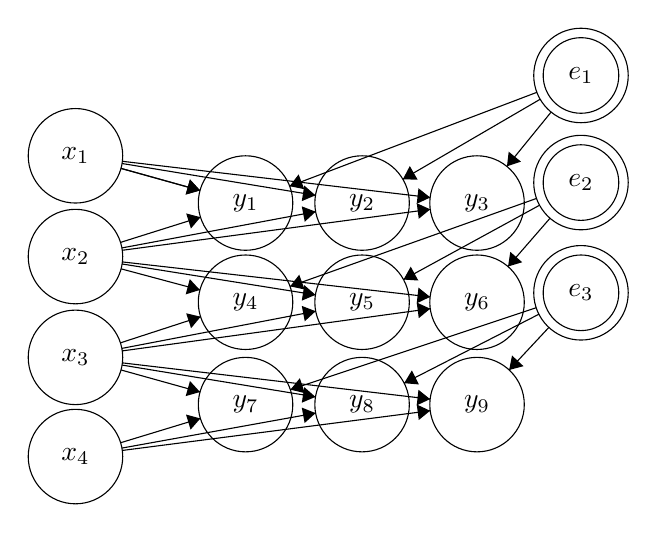
\begin{tikzpicture}[scale=0.2]
		\tikzstyle{every node}+=[inner sep=0pt]
		\draw [black] (8,-12.4) circle (3);
		\draw (8,-12.4) node {$x_1$};
		\draw [black] (8,-18.8) circle (3);
		\draw (8,-18.8) node {$x_2$};
		\draw [black] (8,-25.2) circle (3);
		\draw (8,-25.2) node {$x_3$};
		\draw [black] (8,-31.5) circle (3);
		\draw (8,-31.5) node {$x_4$};
		\draw [black] (18.8,-15.4) circle (3);
		\draw (18.8,-15.4) node {$y_1$};
		\draw [black] (33.5,-15.4) circle (3);
		\draw (33.5,-15.4) node {$y_3$};
		\draw [black] (26.2,-15.4) circle (3);
		\draw (26.2,-15.4) node {$y_2$};
		\draw [black] (18.8,-21.7) circle (3);
		\draw (18.8,-21.7) node {$y_4$};
		\draw [black] (26.2,-21.7) circle (3);
		\draw (26.2,-21.7) node {$y_5$};
		\draw [black] (33.5,-21.7) circle (3);
		\draw (33.5,-21.7) node {$y_6$};
		\draw [black] (18.8,-28.2) circle (3);
		\draw (18.8,-28.2) node {$y_7$};
		\draw [black] (26.2,-28.2) circle (3);
		\draw (26.2,-28.2) node {$y_8$};
		\draw [black] (33.5,-28.2) circle (3);
		\draw (33.5,-28.2) node {$y_9$};
		\draw [black] (40.1,-7.3) circle (3);
		\draw (40.1,-7.3) node {$e_1$};
		\draw [black] (40.1,-7.3) circle (2.4);
		\draw [black] (40.1,-14.1) circle (3);
		\draw (40.1,-14.1) node {$e_2$};
		\draw [black] (40.1,-14.1) circle (2.4);
		\draw [black] (40.1,-21.1) circle (3);
		\draw (40.1,-21.1) node {$e_3$};
		\draw [black] (40.1,-21.1) circle (2.4);
		\draw [black] (10.89,-13.2) -- (15.91,-14.6);
		\fill [black] (15.91,-14.6) -- (15.27,-13.9) -- (15,-14.86);
		\draw [black] (10.86,-17.9) -- (15.94,-16.3);
		\fill [black] (15.94,-16.3) -- (15.03,-16.06) -- (15.33,-17.02);
		\draw [black] (10.89,-13.2) -- (15.91,-14.6);
		\fill [black] (15.91,-14.6) -- (15.27,-13.9) -- (15,-14.86);
		\draw [black] (10.96,-12.89) -- (23.24,-14.91);
		\fill [black] (23.24,-14.91) -- (22.53,-14.29) -- (22.37,-15.28);
		\draw [black] (10.95,-18.25) -- (23.25,-15.95);
		\fill [black] (23.25,-15.95) -- (22.37,-15.61) -- (22.56,-16.59);
		\draw [black] (10.98,-12.75) -- (30.52,-15.05);
		\fill [black] (30.52,-15.05) -- (29.78,-14.46) -- (29.67,-15.45);
		\draw [black] (10.97,-18.4) -- (30.53,-15.8);
		\fill [black] (30.53,-15.8) -- (29.67,-15.41) -- (29.8,-16.4);
		\draw [black] (37.3,-8.37) -- (21.6,-14.33);
		\fill [black] (21.6,-14.33) -- (22.53,-14.52) -- (22.17,-13.58);
		\draw [black] (37.51,-8.81) -- (28.79,-13.89);
		\fill [black] (28.79,-13.89) -- (29.73,-13.92) -- (29.23,-13.05);
		\draw [black] (38.2,-9.63) -- (35.4,-13.07);
		\fill [black] (35.4,-13.07) -- (36.29,-12.77) -- (35.51,-12.14);
		\draw [black] (37.47,-15.54) -- (28.83,-20.26);
		\fill [black] (28.83,-20.26) -- (29.77,-20.32) -- (29.29,-19.44);
		\draw [black] (38.13,-16.37) -- (35.47,-19.43);
		\fill [black] (35.47,-19.43) -- (36.37,-19.16) -- (35.61,-18.5);
		\draw [black] (37.27,-15.11) -- (21.63,-20.69);
		\fill [black] (21.63,-20.69) -- (22.55,-20.89) -- (22.21,-19.95);
		\draw [black] (38.06,-23.3) -- (35.54,-26);
		\fill [black] (35.54,-26) -- (36.45,-25.76) -- (35.72,-25.08);
		\draw [black] (37.43,-22.46) -- (28.87,-26.84);
		\fill [black] (28.87,-26.84) -- (29.81,-26.92) -- (29.36,-26.03);
		\draw [black] (37.25,-22.05) -- (21.65,-27.25);
		\fill [black] (21.65,-27.25) -- (22.56,-27.47) -- (22.25,-26.52);
		\draw [black] (10.9,-19.58) -- (15.9,-20.92);
		\fill [black] (15.9,-20.92) -- (15.26,-20.23) -- (15,-21.2);
		\draw [black] (10.85,-24.28) -- (15.95,-22.62);
		\fill [black] (15.95,-22.62) -- (15.03,-22.4) -- (15.34,-23.35);
		\draw [black] (10.96,-19.27) -- (23.24,-21.23);
		\fill [black] (23.24,-21.23) -- (22.53,-20.61) -- (22.37,-21.6);
		\draw [black] (10.95,-24.63) -- (23.25,-22.27);
		\fill [black] (23.25,-22.27) -- (22.37,-21.93) -- (22.56,-22.91);
		\draw [black] (10.98,-19.14) -- (30.52,-21.36);
		\fill [black] (30.52,-21.36) -- (29.78,-20.77) -- (29.67,-21.77);
		\draw [black] (10.97,-24.79) -- (30.53,-22.11);
		\fill [black] (30.53,-22.11) -- (29.67,-21.72) -- (29.8,-22.71);
		\draw [black] (10.89,-26) -- (15.91,-27.4);
		\fill [black] (15.91,-27.4) -- (15.27,-26.7) -- (15,-27.66);
		\draw [black] (10.87,-30.62) -- (15.93,-29.08);
		\fill [black] (15.93,-29.08) -- (15.02,-28.83) -- (15.31,-29.79);
		\draw [black] (10.96,-25.69) -- (23.24,-27.71);
		\fill [black] (23.24,-27.71) -- (22.53,-27.09) -- (22.37,-28.08);
		\draw [black] (10.95,-30.96) -- (23.25,-28.74);
		\fill [black] (23.25,-28.74) -- (22.37,-28.39) -- (22.55,-29.37);
		\draw [black] (10.98,-25.55) -- (30.52,-27.85);
		\fill [black] (30.52,-27.85) -- (29.78,-27.26) -- (29.67,-28.25);
		\draw [black] (10.98,-31.11) -- (30.52,-28.59);
		\fill [black] (30.52,-28.59) -- (29.67,-28.19) -- (29.8,-29.18);
	\end{tikzpicture}
	\caption{A single layer of ECC with one-dimensional convolution. The input size is $4$ columns, each with one channel. The hidden layer has $3$ columns, each with $3$ channels. The neurons within the same column are all mutually exclusive. Every hidden column draws input from two input columns around it, meaning that in this case the kernel size is $2$. The stride is $0$. }
	\label{fig:ecc_conv_machine}
\end{figure} 
While in deep learning $G$-equivariance is a property of the network $f$, ECC flip this notion ``upside down'' and states that distribution $p$ should $G$-invariant. If $p(x.g)=p(x)$ holds, then the Bayesian decomposition
\[
p(x.g) = p(x) = \sum_{j=1}^m q(x|y_j)p(y_j)  
\]
will be the same for every convolutional column. In fact, they would be exactly the same if the process of learning was deterministic. The learning algorithm for ECC networks is stochastic, meaning that re-running training on the same distribution $p(x)$ multiple times will not yield ``exactly the same'' results, but there will be high correlation between them.
As an example, consider the network from figure \ref{fig:ecc_conv_machine}. Both $[y_1,y_2,y_3]$ and $[y_4,y_5,y_6]$ will develop similar clusterings of $[x_1,x_2]$ and $[x_2,x_3]$ respectively
\begin{gather*}
	p(\boldsymbol{x}) = p(\boldsymbol{x}|y_1)p(y_1)+  p(\boldsymbol{x}|y_2)p(y_2)+  p(\boldsymbol{x}|y_3)p(y_3)\text{ where }\boldsymbol{x}=[x_1,x_2] \\
	p(\boldsymbol{x}) = p(\boldsymbol{x}|y_4)p(y_4)+  p(\boldsymbol{x}|y_5)p(y_5)+  p(\boldsymbol{x}|y_6)p(y_6)\text{ where }\boldsymbol{x}=[x_2,x_3]
\end{gather*}
They will be approximately equal  (correlated)
\[p(\boldsymbol{x}|y_2) \approx p(\boldsymbol{x}|y_{\sigma(4)}), p(\boldsymbol{x}|y_{3}) \approx p(\boldsymbol{x}|y_{\sigma(5)}),p(\boldsymbol{x}|y_3) \approx p(\boldsymbol{x}|y_{\sigma(6)})\]
up to some permutation $\sigma$. All columns learn independently of each other, thus no weight-sharing is required.

This process is not new. Slow feature analysis and other unsupervised learning algorithms can reproduce this phenomenon, if arranged in a hierarchical structure that uses only local (hebbian) update rules. This approach has an advantage over backpropagation, which needs to evaluate all columns at all layers in order to compute error. With hebbian learning, we can save resources by only training a single column and  duplicating it across the entire first layer, then repeat the process for deeper layers.

Producing symmetries with hierarchical structures has been reinvented many times before, but the novelty of this thesis stems from the mathematical formalization of $p$ as $G$-invariant function and relating $G$ to the reinforcement learning state-space $S$ generated by action space $A$. In biological terms, this would mean that eye movement (actions $A$) is necessary to ensure $p$ is invariant to translation, thus potentially allowing convolutional-like structures to emerge in the brain, without requiring weight-sharing.


\subsection{Experiments}

ECC networks have been implemented and benchmarked to investigate their empirical performance. Figure \ref{fig:receptive_fields} presents receptive fields emerging in one arbitrarily chosen column in each of the first 3 layers of convolutional ECC network. These results have been observed when training all columns in all layers simultaneously on MNIST dataset. 
\begin{figure}[!htbp]
	\centering
	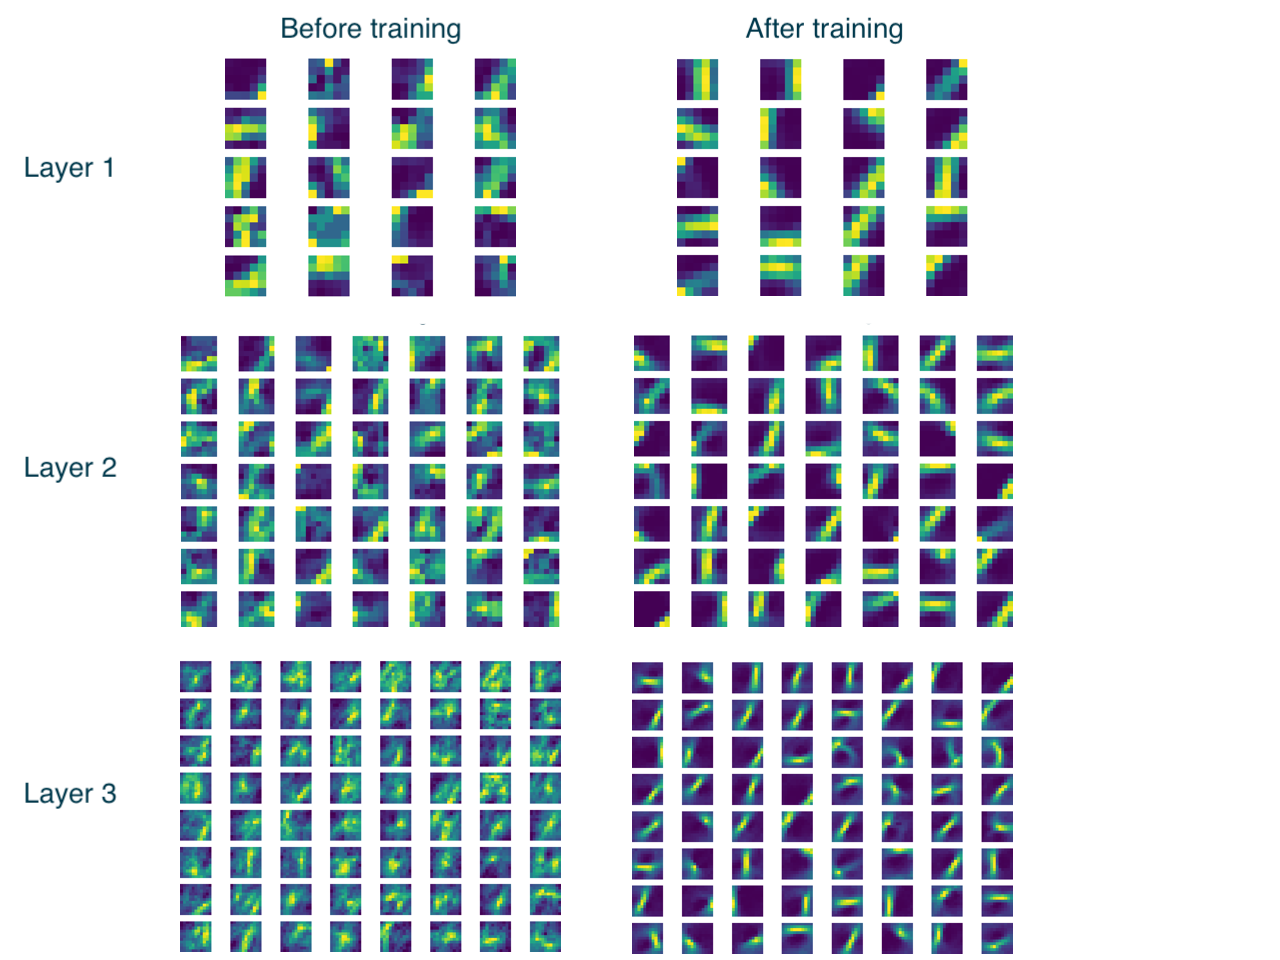
\includegraphics[width=15cm]{receptive_fields}
	\caption{Receptive fields of 20, 49 and 60 neurons from a column in the first, second and third hidden layer.}
	\label{fig:receptive_fields}
\end{figure} 
The convergence speed (fig. \ref{fig:convergence_rate}) is fast and can outperform deep networks.
\begin{figure}[!htbp]
	\centering
	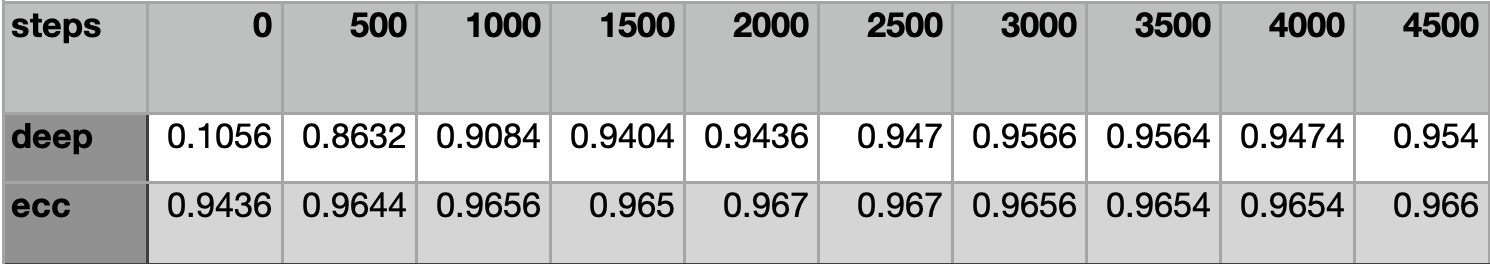
\includegraphics[width=13.5cm]{convergence_rate}
	\caption{Convergence rate of 3-layer ECC compared with 3-layer deep net. A linear classifier head is placed as a fourth layer on both networks and trained independently of the rest. ECC achieves high scores even before learning (only the head was trained), because sparse binary vectors have the effect of random projections.}
	\label{fig:convergence_rate}
\end{figure} 
As the network depth increases, at a certain point the accuracy starts to suffer (table \ref{table:ecc_accuracy}).
\begin{table}[]
	\begin{tabular}{|llllll|}
		\hline
		layer    & 1     & 2     & 3     & 4    & 5    \\ \hline
		channels & 49    & 100   & 144   & 256  & 256  \\ 
		train    & 98\%  & 96\%  & 96\%  & 91\% & 68\% \\ 
		test     & 100\% & 100\% & 100\% & 95\% & 68\% \\ \hline
	\end{tabular}
	\label{table:ecc_accuracy}
	\caption{Accuracy on MNIST observed by adding linear classifier head on top of each layer. This shows a decrease in the quality of learned representations. All layers use convolutional kernel of size 6 by 6. There is no weight sharing.}
\end{table}
This is a sign that only using k-means is not enough and another mechanism might be necessary. All the networks presented so far did not contain any recurrent connections, but they should play a crucial role in biological neurons. When such connections are added between units within the same column, then the weights $W$ converge to autocorrelation matrices (fig \ref{fig:recurrent_connections}).
\begin{figure}[!htbp]
	\centering
	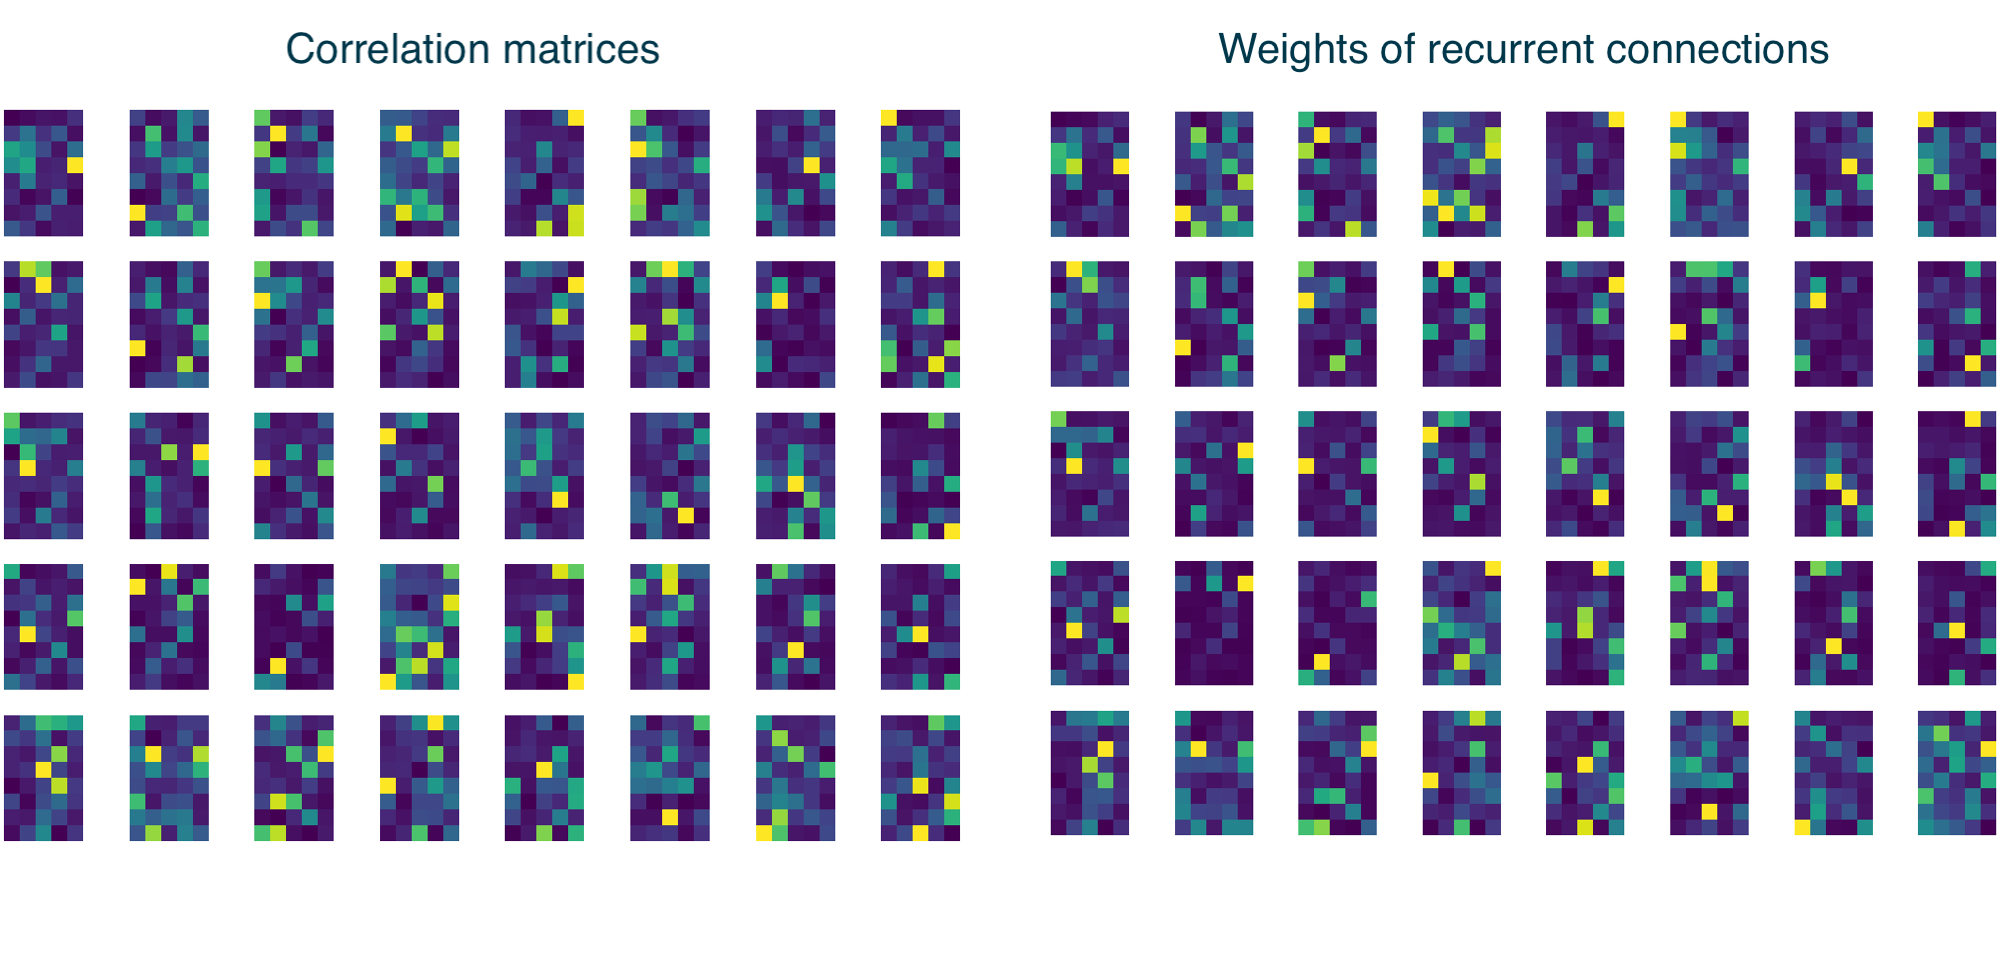
\includegraphics[width=13.5cm]{recurrent_connections}
	\caption{Rows of correlation matrix (left) and weights $W_j$ for each neuron $y_j$ within one column.}
	\label{fig:recurrent_connections}
\end{figure} 
Another important factor in the real brains is the slowness principle. SFA attempts to find functions whose derivative $\langle \dot{y}^2 \rangle$ is minimized, thus ensuring the output varies slowly over time.
In the case of binary vectors, the analogue of $\langle \dot{y}^2 \rangle$   becomes
$(\boldsymbol{y}^{(t+1)}-\boldsymbol{y}^{(t)})^2$, which is equal to the number of differing bits. Minimizing this expression is equivalent to maximizing the number of bits overlapping between consecutive time-steps. ECC networks achieve this effect by randomly fixing hidden layers $\boldsymbol{y}$, preventing the activation patterns from changing in then next step $t+1$ (as if the neurons were repeatedly bursting). Then the input signal $\boldsymbol{x}$ is acted upon with some action $a$. In the case of MNIST, it would be a small random translation. 
As the values $\boldsymbol{y}$ are held fixed, hebbian learning will result in strengthening of connections not only between $\boldsymbol{x}^{(t)}$ and $\boldsymbol{y}^{(t)}$ but also $\boldsymbol{x}^{(t+1)}$ and $\boldsymbol{y}^{(t)}=\boldsymbol{y}^{(t+1)}$. This results in learning transformation-invariant representations (fig. \ref{fig:motor_drift}). 
\begin{figure}[!htbp]
	\centering
	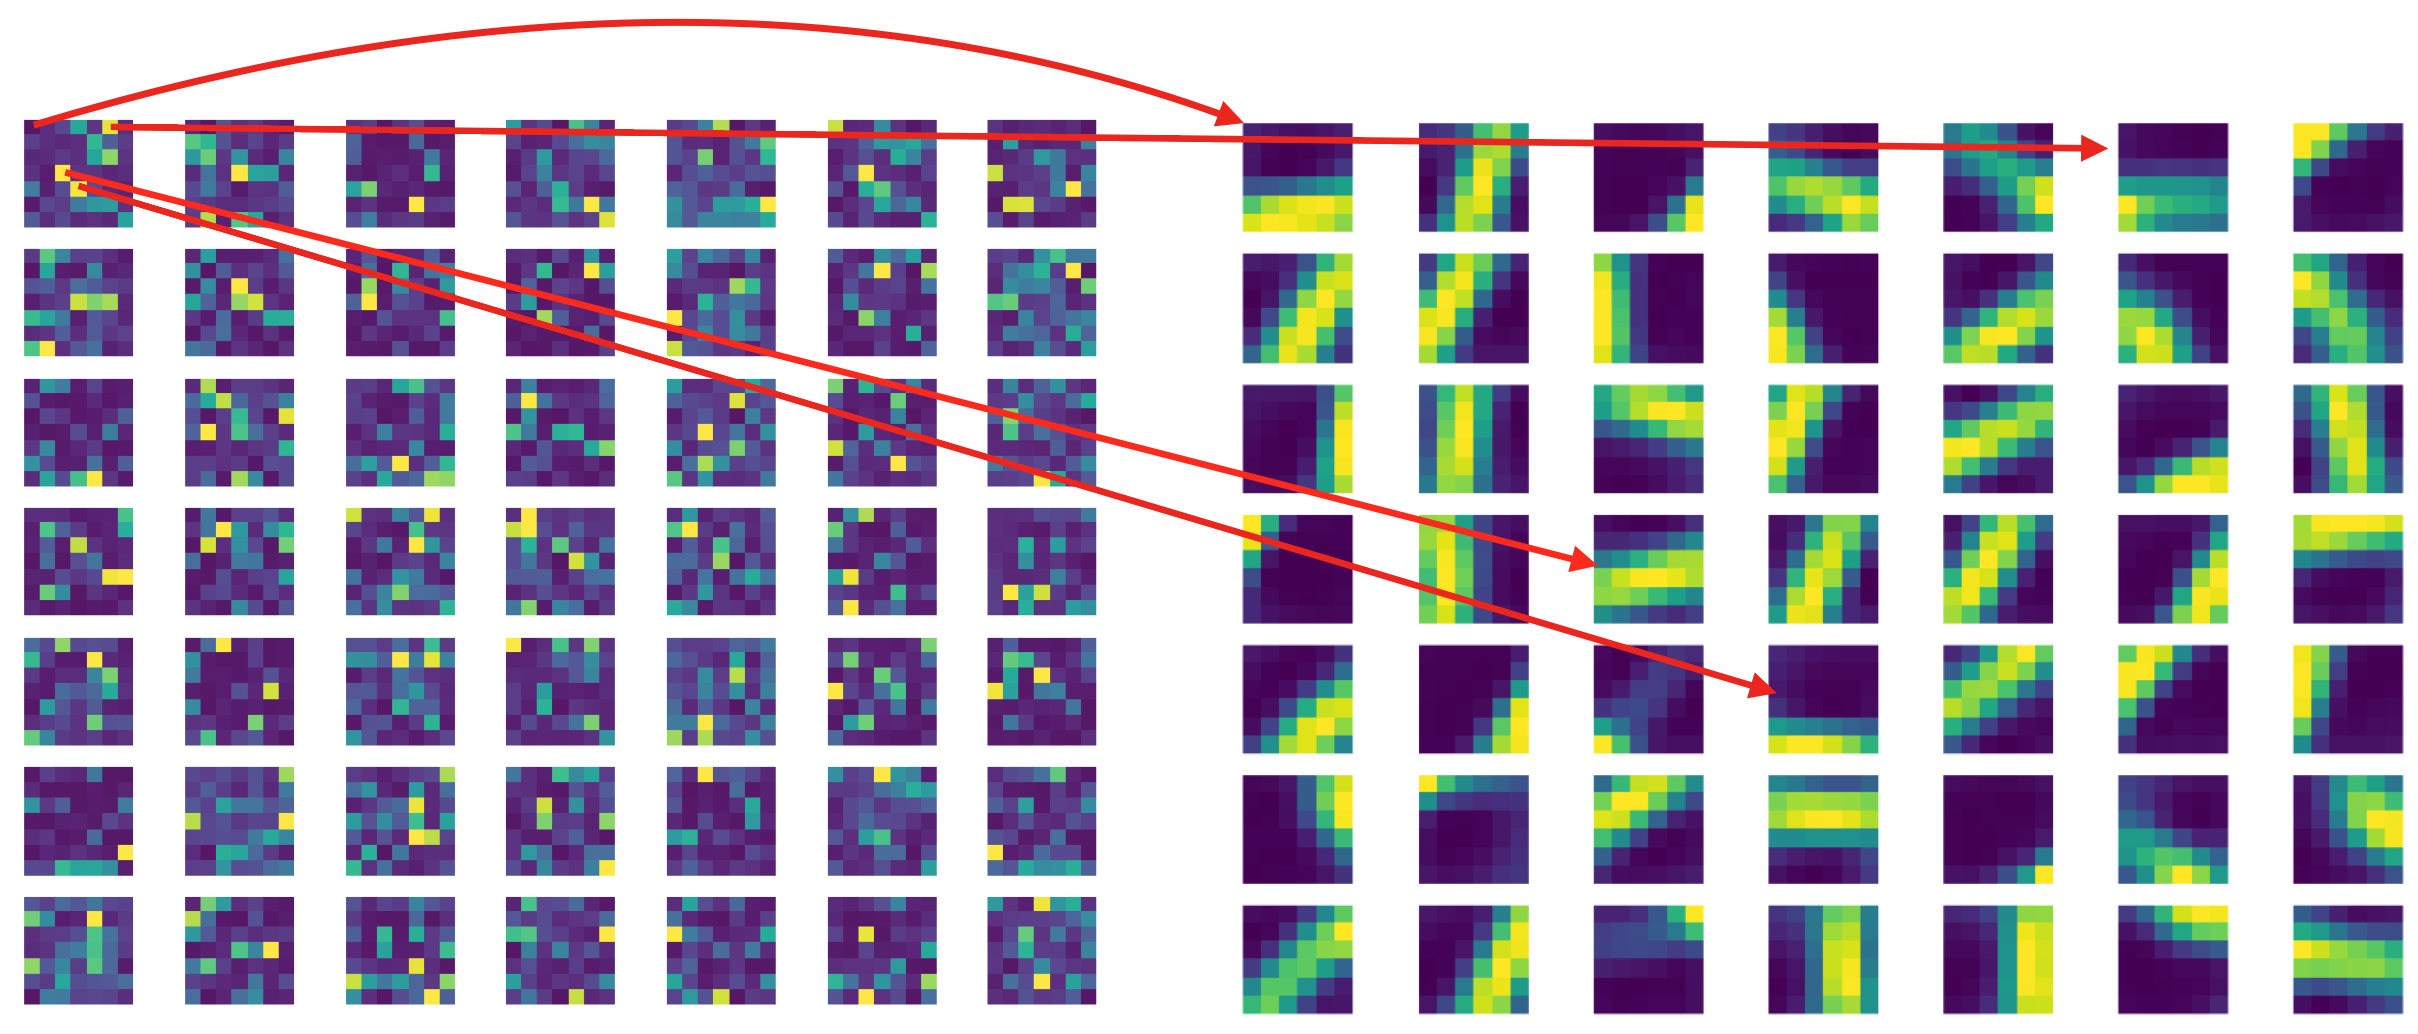
\includegraphics[width=13.5cm]{motor_drift}
	\caption{Weights $W$ in first (left) and second (right) layer emerging when the activations in second layer were randomly frozen during training. Each pixel on the left corresponds to some neuron on the right. The red arrows illustrate how one of the neurons in the second layer has configured itself to detect horizontal lines, regardless of where they are.}
	\label{fig:motor_drift}
\end{figure} 
This approach of leveraging slowness principle has a significant  positive effect on benchmark results (table \ref{table:ecc_accuracy_slow}).
 \begin{table}[]
 	\resizebox{\columnwidth}{!}{%
 	\begin{tabular}{|llllllllllll|}
 		\hline
 		layer    & 1     & 2    & 3     & 4    & 5     & 6    & 7     & 8    & 9    & 10   & 11   \\ \hline
 		channels & 49    & 9    & 144   & 9    & 144   & 16   & 200   & 20   & 256  & 25   & 200  \\
 		train    & 98\%  & 98\% & 98\%  & 97\% & 97\%  & 97\% & 96\%  & 93\% & 90\% & 86\% & 74\% \\
 		test     & 100\% & 99\% & 100\% & 99\% & 100\% & 98\% & 100\% & 95\% & 95\% & 87\% & 75\% \\ \hline
 	\end{tabular}%
    }
 	\label{table:ecc_accuracy_slow}
 	\caption{Each layer with even number uses slowness principle and its activations are randomly fixed. The odd layers do not fix their activations. The kernel size is 6x6 for odd and 1x1 for even layers. An interesting observation is that slowness allows for significant reduction in number of channels.}
 \end{table}

\iffalse
\subsection{Implementation}

The full algorithm written in an online form would look as follows
\begin{lstlisting}
	def ecc($\boldsymbol{x}$,$W$,$u$):
	if $\lVert\boldsymbol{x}\rVert_u$ $\le$ threshold:
	pass    // filter-out noise/empty input
	$k$ = argmax($\boldsymbol{x}W$)
	if learning_enabled:
	$W_k$ = $W_k+\frac{\boldsymbol{x}}{\lVert\boldsymbol{x}\rVert_u}\epsilon$
	$W_k$ = $W_k$ / $\lVert W_k \rVert_u$
	return $k$
\end{lstlisting}
\fi

ECC networks not only converge faster, but their sparsity also allows for significant performance increase. An implementation written in Rust was able to process 2000 MNIST  images  per second on a single thread on 2.7 GHz Intel i5 core. Each image was random patch of 25x25 pixels. The network had 734400 learnable parameters. When learning was enabled, it could train on 1700 images per second. 



\bibliographystyle{BibTeXtran}   % (uses file "BibTeXtran.bst")
\bibliography{BibTeXrefs}    







\end{document}
